%%\documentclass{../doc/tex/feelstyle}
\documentclass[a4paper]{book}
%\documentclass{article}

\usepackage{a4wide}
\usepackage[utf8]{inputenc}

\usepackage{bm}
\usepackage{textcomp}
%\usepackage{lmodern}
%
%%\usepackage{fullpage}
%\usepackage{venturis2}
\usepackage{newcent}
\usepackage[T1]{fontenc}
\usepackage{longtable}
\usepackage{url}
\usepackage{sectsty}
\sectionfont{\sf}
\subsectionfont{\it}
\usepackage[Sonny]{fncychap}
\usepackage{fancyhdr}
\pagestyle{fancyplain}
\lhead{}
\rhead{}

%\fancyhead[RE,LO]{\leftmark}
%\fancyhead[LE,RO]{\thepage}

\usepackage{fancybox}
%\usepackage{fancyvrb}
%\usepackage{color}
\usepackage{exscale,relsize}
\usepackage{xspace}
\usepackage{multicol}
\usepackage{makeidx}
\usepackage{subfigure}
\usepackage{verbatim}
\usepackage{booktabs}
\usepackage[english]{babel}
\usepackage{tabularx}
\usepackage{times}
\usepackage{subfigure}
\usepackage{graphicx}
\graphicspath{%
  {pdfs/}%
  {pngs/}
}
\usepackage{amsmath,amssymb}

\usepackage{xspace}
\usepackage{tikz}
\usetikzlibrary{arrows,patterns,plotmarks,shapes,snakes,er,3d,automata,backgrounds,topaths,trees,petri,mindmap}

\usepackage[colorinlistoftodos]{todonotes}

%
% les trois parties (front, main et back)
%

\renewcommand\backmatter{%
%  \let\minisommaire\null
  \cleardoublepage
 % \@mainmatterfalse
 % \@frontmatterfalse
  \fancyfoot{}
  \fancyhead[LE]{\bfseries\thepage}
  \fancyhead[RO]{\bfseries\thepage}
  \fancyhead[LO]{\bfseries\rightmark}
  \fancyhead[RE]{\bfseries\leftmark}
 % \renewcommand{\toclevel@chapter}{-1}% pour avoir le bookmark au même niveau
 %                                     % que part
}









%-----------------------------------------------------------------------
% index
\usepackage{index}
%-----------------------------------------------------------------------
%
% espace verticale entre les groupes dans l'index
%
\renewcommand\indexspace{\par \vskip 20pt plus5pt minus3pt\relax}
%-----------------------------------------------------------------------


%-----------------------------------------------------------------------
%
% pour avoir un lien correct dans les bookmark du pdf, sur l'index
%
\let\printindexORIG\printindex
\renewcommand{\printindex}{%
  \cleardoublepage
  \phantomsection% création d'une fausse section
  \addcontentsline{toc}{chapter}{Index}
  \printindexORIG}


\AtBeginDocument{%
  \makeindex%
}

%-----------------------------------------------------------------------


%-----------------------------------------------------------------------
% fancyvrb unixcom environment
\usepackage{styles/fvrb}

%-----------------------------------------------------------------------
% nota environment
\usepackage{styles/nota}
%\newcommand{\ficnota}{attention}
%\newcommand{\ficnota}{}
%\newcommand{\ficnote}{note}
\newcommand{\ficnote}{}
%\newcommand{\ficnotahack}{question}
\newcommand{\ficnotahack}{}

\setlength{\largeurnota}{.8cm}
\newenvironment{nota}{%
  \begin{pictonote}{\ficnota}}{\end{pictonote}}
\newenvironment{note}{%
  \begin{pictonote}{\ficnote}}{\end{pictonote}}
\newenvironment{notahack}{%
  \begin{pictonote}{\ficnotahack}}{\end{pictonote}}


\usepackage{xcolor}
\newtheorem{problem}{Problem}
\newtheorem{remark}{Remark}



\definecolor{lbcolor}{rgb}{0.941,0.984,0.941}
\definecolor{cblue}{rgb}{0.,0.0,0.6}

\usepackage[colorlinks=true]{hyperref}
\usepackage{filecontents,listings}
\lstset{language=c++,showspaces=false,showstringspaces=false,captionpos=t,literate={>>}{\ensuremath{>>}}1,mathescape}
%\lstset{float}
\lstset{basicstyle=\small\ttfamily}
\lstset{lineskip=-2pt}
\lstset{keywordstyle=\color{red}\bfseries}
%\lstset{keywordstyle=\mdseries\color{red}}
\lstset{emph={inline},emphstyle=\color{red}\bfseries}
%\lstset{stringstyle=\ttfamily}
\lstset{commentstyle=\ttfamily\color{cblue}}
\lstset{backgroundcolor=\color{lbcolor},rulecolor=}
%\lstset{numbers=left}
%\lstset{numbers={none}}
%\lstset{numberstyle=\tiny}
%\lstset{numbersep=1pt}
\lstset{frame=single,framerule=0.5pt}
\lstset{belowskip=\smallskipamount}
\lstset{aboveskip=\smallskipamount}
\lstset{emph={constant,cst,cst_ref,constant_ref,val,integrate,on,grad,gradt,gradv,dot,id,dx,dy,dz,idt,dxt,dyt,dzt,div,divt,idv,dxv,dyv,dzv,dn,dnt,mass,stiffness,trans,trace,jump,jumpt,average,averaget,maxface,project,P,Px,Py,Pz,h,H,Hface,hFace,N,Nx,Ny,Nz,sqrt,sin,cos,min,max,abs,sign,pow,chi,exp,log,form1,form2, FunctionSpace, bases,
prod,element_prod, range, subrange, inner_prod,unite,elements,markedelements,markedfaces,boundaryfaces,faces,internalelements,boundaryelements,edges,boundaryedges,_Q},emphstyle=\color{blue}}
\lstset{includerangemarker=false,rangeprefix=\/\/\#\ ,% curly left brace plus space
  rangesuffix=\ \#}% space plus curly right brace

\newcommand{\feelchapter}[4]{\chapter{#1 \\ \small{\rm By #3}} \vspace{-1cm}
                              Chapter ref: \textbf{[#4]} \label{chap:#4} \vspace{1cm} \chead[#2]{#3}}
\newcommand{\feelappendix}[2]{\chapter{#1} \chead{#2}}


\newcommand{\acos}{\ensuremath{\mathrm{acos}}\xspace}
\newcommand{\asin}{\ensuremath{\mathrm{asin}}\xspace}
\newcommand{\atan}{\ensuremath{\mathrm{atan}}\xspace}
%\newcommand{\tanh}{\ensuremath{\mathrm{tanh}}\xspace}
\newcommand{\cc}{{\sl\sffamily C}\xspace}
\newcommand{\cpp}{C{\hspace{-.3em}\vspace{-.2em}\tiny++}\xspace}
\newcommand{\polyP}[1]{\ensuremath{\mathbb{P}_{#1}}\xspace}
\newcommand{\feel}{\textsc{Feel++}\xspace}
\newcommand{\Feel}{\textsc{Feel++}\xspace}
\newcommand{\FEEL}{\textsc{Feel++}\xspace}
\newcommand{\cmake}{\texttt{cmake}\xspace}
\newcommand{\ccmake}{\texttt{ccmake}\xspace}


\newcommand{\In}{\operatorname{in}}
\newcommand{\Out}{\operatorname{out}}

\newcommand{\setR}[1]{{\ensuremath{\mathbb{R}^{#1}}}\xspace}
\newcommand{\Om}[1]{{\ensuremath{\Omega^{#1}}}\xspace}
\newcommand{\Omst}{{\ensuremath{\Omega^{\text{st}}}}\xspace}

\newcommand{\aloc}[1]{{\ensuremath{a^{#1}_{\text{loc}}}}\xspace}
\newcommand{\iloc}{{\ensuremath{i_{\text{loc}}}}\xspace}
\newcommand{\jloc}{{\ensuremath{j_{\text{loc}}}}\xspace}
\newcommand{\nldof}{{\ensuremath{N_{\text{localdof}}}}\xspace}
\newcommand{\ngdof}{{\ensuremath{N_{\text{geomdof}}}}\xspace}
\newcommand{\ndof}{{\ensuremath{N_{\text{dof}}}}\xspace}
\newcommand{\nel}{{\ensuremath{N_{\text{el}}}}\xspace}
\newcommand{\PS}[1]{{\ensuremath{\mathbb{P}_N}}\xspace}
\newcommand{\QS}[1]{{\ensuremath{\mathbb{Q}_N}}\xspace}
\newcommand{\GT}[1]{{\ensuremath{\mathcal{T}^{#1}}}\xspace}
\newcommand{\GQ}[1]{{\ensuremath{\mathcal{Q}^{#1}}}\xspace}

%% Macros
\renewcommand{\div}{\operatorname{div}}
\newcommand{\rot}{\operatorname{rot}}

\newcommand{\meter}{\ensuremath{\mathrm{m}}\xspace}

\newcommand{\PP}[1]{{\ensuremath{\mathbb{P}_{#1}}}\xspace}

\newcommand{\pHat}{{\ensuremath{\Hat{p}}}\xspace}
\newcommand{\xHat}{{\ensuremath{\Hat{x}}}\xspace}
\newcommand{\wHat}{{\ensuremath{\Hat{w}}}\xspace}
\newcommand{\THat}{{\ensuremath{\Hat{T}}}\xspace}
\newcommand{\Pk}{\ensuremath{\mathbb{P}_k(K)}\xspace}
\newcommand{\PN}{\ensuremath{\mathbb{P}_N(K)}\xspace}
\newcommand{\Pkmun}{\ensuremath{\mathbb{P}_{k-1}(K)}\xspace}

\InputIfFileExists{version}{}{\def\feelversion{\texttt{x.y.z}}}
\title{Feel Manual\\
A Library for Finite and Spectral Element Methods in 1D, 2D and 3D\\
{\small \feelversion }}
\author{Christophe Prud'homme\thanks{Université de Grenoble,
51, rue des Mathématiques, BP53,38041 Grenoble}}
\date{}

\thispagestyle{empty}
\begin{document}
\thispagestyle{empty}


% \CssFile
% /* css.sty */
% body { width: 75% }
% h1,h2,h3,h4,h5,h6,pre,code,p {font-size: 1em; font-weight: normal; }
% dl,li,dt,dd,h1,h2,h3,h4,h5,h6,pre,form,body,html,p,blockquote,fieldset,input {margin: 0; padding: 0;}
% h2,h3,h4,h5,h6 { color: #B30000; }
% h1 { color: #FFB267; }
% h2 { border-bottom: 1px dotted #FFB267; border-left: 1px dotted #FFB267; }
% h3 { border-bottom: 1px dotted #D95934; }

% div.lstlisting{background: #eee; border: thin solid #000;  }
% div.lstinputlisting{background: #eee; border: thin solid #000; }

% \EndCssFile

%\maketitle
\begin{figure}[!h]
\centering
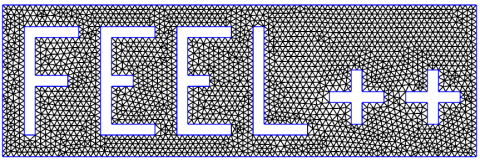
\includegraphics[width=.60\linewidth]{feel_logo.png}
\end{figure}


\begin{center}
  {\Large
    FEEL MANUAL \\
    A LIBRARY FOR \\
    FINITE AND SPECTRAL ELEMENT METHODS IN \\
    1D, 2D AND 3D\\
    \bigskip
    {\small Version \feelversion }}\\[0.6cm]
    Editor\\
  Christophe \textsc{Prud'homme}\\
  \feel Consortium\\
  \texttt{christophe.prudhomme@feelpp.org}\\
  \par\vspace{2cm}

  % \begin{flushright}
  %   \footnotesize
  %   Version du \feelsvndate\\
  %   Revision \feelsvnrevision
  % \end{flushright}
  % \par\vspace{5cm}

  % \centerline{\begin{minipage}[l]{0.35\linewidth}
  %   
\includegraphics[width=.7\linewidth]{logo-ujf}
  % \end{minipage}
  % \begin{minipage}[r]{0.35\linewidth}
  %   
\includegraphics[width=.7\linewidth]{logo-ljk}
  % \end{minipage}}


\end{center}

\vfill \mbox{} \clearpage

\thispagestyle{empty}


\vfill
Permission is granted to copy, distribute and/or modify this document
under the terms of the GNU Free Documentation License, Version 1.2
or any later version published by the Free Software Foundation;
with no Invariant Sections, no Front-Cover Texts, and no Back-Cover Texts.
A copy of the license is included in the section entitled "GNU
Free Documentation License".

\newpage

\tableofcontents

\part{Tutorial}
\label{part:tutorial}

\feelchapter{Building Feel++}
            {Building Feel++}
            {Christophe Prud'homme, Baptiste Morin}
            {tutorial-building}

\section{Getting the source via an archive}
\label{sec:getting-source-via-1}

\feel is distributed as a tarball once in a while. The tarballs are available
at
\begin{center}
  \href{http://code.google.com/p/feelpp/}{http://code.google.com/p/feelpp/}
\end{center}
Download the latest tarball.

\begin{unixcom}
  tar -xzf feelpp-0.92.0.tar.gz
  cd feel-0.92.0
\end{unixcom}


\section{Getting the source via Git}
\label{sec:getting-source-via}
In order to download the sources of \feel, you can download it directly from the source depository
thanks to Git. To make it possible, you can download them anonymously or with an account in Github that you have created. As an open-source project, we strongly suggest you to create an account and take part of the project with sharing your ideas, developments or suggests. If you're interested to participate and become a \feel developer, please don't hesitate to see how it works in the appendix ~\ref{feeldevel}. For now, if you want to get the sources without an account, open a command-line and type
\begin{unixcom}
    git clone https://github.com/feelpp/feelpp.git
\end{unixcom}
then you can go to the \feel top directory with
\begin{unixcom}
		cd feel
\end{unixcom}
You should obtain furthers directories such as :
\begin{lstlisting}[language=sh]
applications/   # functional applications
benchmarks/  # applications under test
cmake/   # do not touch, used for compilation
contrib/
doc/   # tutorial and examples
feel/   # Feel++ library
ports/   # used for Mac OS X installation
research/   # research projects using Feel++
testsuite/ # Feel++ unit tests testsuite
CMakeListe.txt   # the file for cmake to build, do not modify
...
\end{lstlisting}

\section{Unix : dependencies}
\label{sec:about-dependencies}

In order to install \feel on Unix systems (other than Mac OS X, in you have a Macintosh, please go to ~\ref{macosx}), you have to install many dependencies
before. Those libraries and programs are necessary for the
compilation and installation of the \feel librairies.
This is the list of all the librairies you must have installed on your
computer, and the \lstinline|*-dev| packages for some of them. \\
\underline{Required packages}:
\begin{itemize}
\item g++ ($4.5$, $4.6$ and $4.7$) or clang++ ($\geqslant 3.1$)
\item MPI : openmpi (preferred) or mpich
\item Boost ($\geq$1.39)
\item Petsc ($\geq$2.3.3)
\item Cmake ($\geq$2.6)
\item Gmsh\footnote{Gmsh is a pre/post processing software for scientific
computing available at \url{http://www.geuz.org/gmsh}}
\item Libxml2
\end{itemize}
\underline{Optional packages}:
\begin{itemize}
\item Superlu
\item Suitesparse(umfpack)
\item Metis: scoth with the metis interface (preferred), metis (non-free)
\item Trilinos ($\geq$8.0.8)
\item Google perftools
\item Paraview\footnote{Paraview is a few parallel scientific data
    visualisation plateform, \url{http://www.paraview.org}}, this is
  not stricly required to run \feel programs but it is somehow
  necessary for visualisation
\item Python ($\geq$ 2.5) for the validation tools
\end{itemize}
Note that all these packages are available under Debian/GNU/Linux and
Ubuntu. They should be available. Once you have installed those dependencies, you can jump to ~\ref{compilingfeel}.

\section{\feel on Debian and Ubuntu}
\label{sec:feel-debian-ubuntu}

\subsection{Debian}

Debian is the platform of choice for \feel, it was developed mainly on it. The commands to install \feel on Debian are
\begin{unixcom}
  sudo apt-get update
  sudo apt-get install feel++-apps libfeel-dev feel++-doc
\end{unixcom}


The interested user is encourage to follow the \feel PTS page
\begin{itemize}
\item \feel \href{http://packages.qa.debian.org/f/feel%2B%2B.html}{Debian Packages Tracking System}
\end{itemize}

At the moment \feel compiles and is available on the following Debian
plateforms:
\begin{itemize}
\item \feel \href{https://buildd.debian.org/status/package.php?p=feel%2b%2b}{Buildd results}
\end{itemize}

\subsection{Ubuntu}

\feel was uploaded in the distribution Ubuntu-Natty (11.04) for the first
time. The commands to install \feel on Ubuntu are
\begin{unixcom}
  sudo apt-get update
  sudo apt-get install feel++-apps libfeel-dev feel++-doc
\end{unixcom}
The interested user might want to follow the Ubuntu Launchpad \feel page in
order to know what is going on with \feel on Ubuntu
\begin{itemize}
\item \feel \href{https://launchpad.net/ubuntu/+source/feel++}{Ubuntu Source
  Page for all Ubuntu versions}
\end{itemize}


\section{\Feel on Mac OS X}
\label{macosx}
\feel is also working on Mac operating systems. The way to make it work is quite different.

\subsection{Compilers}

In order to \feel and \cmake work properly, you have to install differents compilers :
\begin{itemize}
\item Gcc \\
  The first step is to install the latest version of Xcode. If your computer is
  recent, you can install it with your DVD that came with your machine (not the
  OS DVD, but the applications one). You don't have to install the complete
  Xcode (you can uncheck iOS SDK for example, it's not necessary here and
  requiers a lot of memory). Xcode will provide your computer all basic tools to
  compile such as gcc 4.2. It's the first step, you'll see later how to easily
  install gcc 4.5 or later using MacPorts.
\item Fortran \\
  To build the Makefiles, \cmake will need a Fortran compiler. To make it works,
  please go to \href{http://hpc.sourceforge.net/}{SourceForge.net} and download
  \lstinline|gfortran-snwleo-intel-bin.tar.gz| which is the fortran compiler
  only (from now, don't download the complete install with gcc 4.6 because Feel
  needs gcc 4.5 or later). To install it, go to the directory where you have
  downloaded the file and type in a command-line
\begin{unixcom}
		sudo tar -xvf gfortran-snwleo-intel-bin.tar -C /
\end{unixcom}

\end{itemize}

\subsection{MacPorts}

\paragraph{Introduction}
MacPorts is an open-source community projet which aims to design an easy-to-use
system for compiling, installing and upgrading open-source softwares on Mac OS X
operating system. It is distributed under
\href{http://opensource.org/licenses/bsd-license.php}{BSD License} and
facilitate the access to thousands of ports (softwares) without installing or
compiling open-source softwares.  MacPorts provides a single software tree which
includes the latest stable releases of approximately 8050 ports targeting the
current Mac OS X release (10.6 or 10.5). If you want more information, please
visite their \href{http://www.macports.org/}{website}.

\paragraph{Installation}
To install the latest version of MacPorts, please go to
\href{http://www.macports.org/install.php}{Installing MacPorts} page and follow
the instructions. The simplest way is to download the $dmg$ disk image
corresponding to your version of Mac OS X. It is recommended that you install
X11 (X Window System) which is normally used to display X11
applications.%, and also the Xcode Tools (only the developer tools, iOS SDK is not required).

If you have installed with the package installer
(\lstinline|MacPorts-1.x.x.dmg|) that means MacPorts will be installed in
\lstinline|/opt/local|. From now on we will suppose that macports has been
installed in \lstinline|/opt/local| which is the default MacPorts location. Note
that from now on, all tools installed by MacPorts will be installed in
\lstinline!/opt/local/bin! or \lstinline!/opt/local/sbin! for example (that's
here you'll find gcc4.5 or later e.g \lstinline!/opt/local/bin/g++-mp-4.5! once being
installed).%At the end of the installation, you can check if your PATH has been upgraded by the command \lstinline|echo $PATH| which should return a line containing \lstinline|/opt/local/bin:/opt/local/sbin|.

\paragraph{Key commands}
In your command-line, the software MacPorts is called by the command \lstinline|port|.
Here is a list of key commands for using MacPorts, if you want more informations please go to \href{http://guide.macports.org/#using.port}{MacPorts Commands}.
\begin{itemize}
\item \lstinline|sudo port -v selfupdate|
	This action should be used regularly to update the local tree with the global MacPorts ports. The option \lstinline|-v| enables verbose which generates verbose messages.
\item \lstinline|port info flowd|
	This action is used to get information about a port (description, license, maintainer, etc.)
\item \lstinline|sudo port install mypackage|
	This action install the port mypackage
\item \lstinline|sudo port uninstall mypackage|
	This action uninstall the port mypackage
\item \lstinline|port installed|
	This action displays all ports installed and their versions, variants and activation status. You can also use the \lstinline|-v| option to also display the platform and CPU architecture(s) for which the ports were built, and any variants which were explicitly negated.
\item \lstinline|sudo port upgrade mypackage|
	This action updgrades installed ports and their dependencies when a \lstinline|Portfile| in the repository has been updated. To avoid the upgrade of a port's dependencies, use the option \lstinline|-n|.
\end{itemize}

\paragraph{Portfile}
A Portfile is a TCL script which usually contains simple keyword values and TCL
expressions. Each package/port has a corresponding Portfile but it's only a part
of a port description.  \feel provides some mandatory Portfiles for its
compilation which are either not available in MacPorts or are buggy but \feel
also provides some Portfiles which are already available in MacPorts such as
gmsh or petsc. They usually provide either some fixes to ensure \feel works
properly or new version not yet available in MacPorts.  These Portfiles are
installed in \lstinline|ports/macosx/macports|.


\subsection{MacPorts and \Feel}


To be able to install \feel, add the following line in \lstinline|/opt/local/etc/macports/source.conf|
at the top of the file before any other sources :
\begin{lstlisting}[language=sh]
file:///<path to feel top directory>/ports/macosx/macports
\end{lstlisting}

Once it's done, type in a command-line :
\begin{unixcom}
		cd <your path to feel top directory>/ports/macosx/macports
		portindex -f
\end{unixcom}

You should have an output like this :
\begin{flushleft}
\fbox{
   \begin{minipage}{0.81\textwidth}
      	Reading port index in $<$your path to feel top directory$>$/ports/macosx/macports\\
	Adding port science/feel++ \\
	Adding port science/gmsh \\
	Adding port science/petsc \\ \\
	Total number of ports parsed:   3\\
	Ports successfully parsed:      3\\
	Ports failed:                   0\\
	Up-to-date ports skipped:       0
   \end{minipage}
}
\end{flushleft}
Your are now able to type
\begin{unixcom}
		sudo port install feel++
\end{unixcom}
It might take some time (possibly an entire day) to compile all the requirements for \feel
to compile properly. If you have several cores on your MacBook Pro, iMac or MacBook
we suggest that you configure macports to use all or some of them.
To do that uncomment the following line in the file  \lstinline|/opt/local/etc/macports/macports.conf|
\begin{flushleft}
\begin{lstlisting}[language=sh]
buildmakejobs	0 $\#$ all the cores
\end{lstlisting}
\end{flushleft}
At the end of the \lstinline|sudo port install feel++|, you have all
dependencies installed. To build all the Makefile, \cmake is automatically
launched but can have some libraries may not be found but they are not mandatory
for build Feel++, only the features related to the missing libraries will be
missing.

\subsection{PETSc and SLEPc on Snow Leopard and Lion}
We have heard about issues with petsc and slepc with some new MacBook Pro with
Snow Leopard while they are being installed with the command
\begin{unixcom}
  sudo port install feel++
\end{unixcom}
If it's the case, that probably means there is an issue with
atlas. If atlas is already installed, you have to unsinstall it (be careful
with dependencies, they also have to be uninstalled). Once it's done, you should
do
\begin{unixcom}
		cd <path to feel top directory>/ports/macosx/macports
		portindex -f
\end{unixcom}

then type in the exact same order :
\begin{unixcom}
		sudo port uninstall slepc
		sudo port uninstall petsc
		sudo port install -d petsc
		sudo port install slepc
\end{unixcom}
Then add to you shell script environment (e.g. for Bash shells \lstinline|.bashrc| or
\lstinline|.profile| or for CSh shells \lstinline|.tcshrc|)
\begin{unixcom}
  # Sh based shell
  export PETSC_DIR=/opt/local/lib/petsc
  export SLEPC_DIR=/opt/local/lib/petsc

  # CSh based shell
  setenv PETSC_DIR /opt/local/lib/petsc
  setenv SLEPC_DIR /opt/local/lib/petsc
\end{unixcom}
and type once again
\begin{unixcom}
		sudo port install feel++
\end{unixcom}

\noindent In that order, slepc and petsc will be installed before atlas, and feel will be properly installed.

\subsection{Missing ports}
\cmake can build Makefiles even if some packages are missing (latex2html, VTK
...). It's not necessary to install them but you can complete the installation
with MacPorts, \cmake will find them by itself once they have been installed.

\section{Compiling Feel++}
\label{compilingfeel}
Feel build system uses \cmake\index{cmake}\footnote{\url{http://www.cmake.org}}
as its build system. Check that \cmake is using gcc4.5 (or a higher version) 
or clang++ as C++ compiler
(you can use the option \lstinline|CMAKE_CXX_COMPILER=<path>/g++-4.5| where the
\lstinline|path| depends on your OS, it's probably \lstinline|/usr/bin| or
\lstinline|/opt/local/bin| but you can also change it with the command \lstinline|ccmake|
and press \lstinline|t| for advanced options).  
\feel, using \cmake, can be built either in source and out of source and different
build type:
\begin{itemize}
\item minsizerel : minimal size release
\item release release
\item debug : debug
\item none(default)
\end{itemize}

\paragraph{CMake Out Source Build (preferred)}
The best way is to have a directory (\lstinline|FEEL| for example) in which you have : \\
\begin{lstlisting}
	feel/
\end{lstlisting}
where \lstinline|feel| is the top directory where the source have been downloaded. Placed in \lstinline|FEEL|, you can create the build directory (\lstinline|feel.opt| for example) and lauch cmake with :
\begin{unixcom}
  mkdir feel.opt
  cd feel.opt
  cmake <directory where the feel source are>
  # e.g cmake ../feel if feel.opt is at the same
  # directory level as feel
\end{unixcom}
you can customize the build type:
\begin{unixcom}
  # Choose g++ release
  cmake -CMAKE_CXX_COMPILER=/usr/bin/g++-4.5
  # Debug build type (-g...)
  cmake -D CMAKE_BUILD_TYPE=Debug
  # Release build type (-O3...)
  cmake -D CMAKE_BUILD_TYPE=Release
  ...
\end{unixcom}
Once Cmake has made its work, you are now able to compile the library with
\begin{unixcom}
		make
\end{unixcom}
\textbf{Important :} from now, all commands should be type in \lstinline|feel.opt| or its subdirectories.


% \subsection{Compiling Feel with the AutoTools}

% Go in the same folder in wich you have done the checkout and type the following
% commands :

% \subsubsection{From tarball}
% \label{sec:from-tarball}

% The steps are as follows to configure the \feel Development Plateform

% \begin{unixcom}
%   cd feel-x.y.z
%   mkdir opt
%   cd opt

%   ../configure --enable-opt2
% \end{unixcom}

% Then type
% \begin{unixcom}
%   make
% \end{unixcom}

% to compile the library and the tutorial. And finally type
% \begin{unixcom}
%   make check
% \end{unixcom}
% In order to compile the testsuite, the examples and the benchmarks and
% execute some of them to verity that the \feel library is functional.


% \subsubsection{From subversion}
% \label{sec:from-subversion}

% The steps are as follows to configure the \feel Development Plateform

% \begin{unixcom}
%   cd feel
%   make -f Makefile.dist
%   mkdir opt
%   cd opt

%   ../configure --enable-opt2
% \end{unixcom}

% Then, to build  the \feel library, type
% \begin{unixcom}
%   make
% \end{unixcom}

% And finally to check the library, type
% \begin{unixcom}
%   make check
% \end{unixcom}


% \begin{note}
%   The script \lstinline!configure! supports many command line
%   options. In particular if you are interested in writing some code or
%   examples inside the \feel environment you have to enable the so
%   called \emph{maintainer mode} to ensure that the makefiles are
%   properly regenerated when you modify a \lstinline!Makefile.am! or if
%   you modify \lstinline!configure.ac!, to achieve this type
%   \begin{unixcom}
%     configure --enable-maintainer-mode
%   \end{unixcom}
%   To list all configure options, type
%   \begin{unixcom}
%     configure --help
%   \end{unixcom}
% \end{note}


% \subsubsection{Compiling an extra module}
% \label{sec:compile-an-extra}

% If you work with an extra module, \emph{e.g.} \lstinline!validation!, the steps are as follows
% \begin{unixcom}
% cd feel
% make -f Makefile.dist
% cd benchmarks/validation
% make -f Makefile.dist
% cd ../../..
% mkdir opt
% cd opt
% ../feel/configure --enable-opt2 --enable-maintainer-mode
% make
% make check
% \end{unixcom}


\subsection{Compiling the Feel++ manual}
\label{sec:comp-feel-tutor}
The manual (which includes the tutorial) is edited with \LaTeX  so you need to have installed the \LaTeX  distribution on your computer. \LaTeX  is a high-quality typesetting system, it includes features designed for the production of technical and scientific documentation. There are several ways to make it work, for example you can go on \href{http://www.tug.org/mactex/}{MacTeX website} and follow the instructions to install the distribution. If the command \lstinline|make check| in \lstinline|feel.opt/| has been run before, the tutorial
should be already compiled and ready. The steps are as follows to build the Feel tutorial
\begin{unixcom}
  cd feel.opt/doc/manual
  make pdf
\end{unixcom}
%Here is what the directory should look like
%\begin{unixcom}
%  cd opt/doc/tutorial
%  ls
%
%  laplacian     Makefile      myintegrals   mymesh       pngs/
%  tutorial.blg  tutorial.out  tutorial.toc  laplacian.o  myapp
%  myintegrals.o mymesh.o      stokes.assert tutorial.aux pdfs/ styles/
%  stokes        stokes.o      tutorial.bbl  tutorial.log tutorial.pdf
%\end{unixcom}
The directory \lstinline|doc/manual| contains all examples used in the tutorial. You will see how it works in the following parts.

%%% Local Variables:
%%% coding: utf-8
%%% mode: latex
%%% TeX-PDF-mode: t
%%% TeX-parse-self: t
%%% x-symbol-8bits: nil
%%% TeX-auto-regexp-list: TeX-auto-full-regexp-list
%%% TeX-master: "../feel-manual"
%%% ispell-local-dictionary: "american"
%%% End:


\feelchapter{Getting Started with Feel++}
            {Getting Started with Feel++}
            {Christophe Prud'homme, Baptiste Morin}
            {cha:getting-started}


\section{Creating applications}
\label{sec:creat-appl}


\marginpar{\lstinline!myapp.cpp!}

\subsection{Application and Options}
\label{sec:options}

As a \feel user, the first step in order to use \feel is to create an
application. Before writing anything, you have to include the \lstinline!Application! header and the header which handles the internal \feel options.
%\lstinline!feel/feelcore/application.hpp! and the header which the internal \feel options.
Note that \feel uses the \lstinline!boost::program_options!\footnote{\url{http://www.boost.org/doc/html/program_options.html}} (\verb|po|)
library from Boost to handle its command line options.

\lstinputlisting[linerange=marker1-endmarker1]{myapp.cpp}

Next to ease the programming and reading, we use the \lstinline!using!
\cpp directive to bring the namespace Feel to the current namespace

\begin{lstlisting}
  using namespace Feel;
\end{lstlisting}

Then we define the command line options that the applications will
provide. Note that on the \lstinline!return! line, we incorporate the
options defined internally in \feel.

\lstinputlisting[linerange=marker2-endmarker2]{myapp.cpp}

In the example, we provide the options \lstinline!dt! which takes an
argument, a \lstinline!double! and its default value is \lstinline!1!
if the options is not set by the command line. Then we describe the application by defining a class
\lstinline!AboutData! which will be typically used by the
\lstinline!help! command line options to describe the application


\lstinputlisting[linerange=marker3-endmarker3]{myapp.cpp}


Now we turn to the class \lstinline!MyApp! itself: it derives from
\lstinline!Feel::Application!. This class provides two constructors : one with only description and one with additionnal parameters which enables to add options
\lstinline!argc! and \lstinline!argv!.
%and the \lstinline!AboutData! as well as possibly the description of the command line options \lstinline!Feel::po::option_description!.
This class \lstinline!MyApp! has to redefine the \lstinline!run()! method. It is defined as a pure virtual function in \lstinline!Application!.


\lstinputlisting[linerange=marker4-endmarker4]{myapp.cpp}

The implementation of the constructors is usually simple, we pass the
arguments to the super class \lstinline!Application! that will analyze
them and subsequently provide them with a
\lstinline!Feel::po::variable_map! data structure which operates like
a \lstinline!map!. Have a look at the document \lstinline!boost::program_options!\footnote{\url{http://www.boost.org/doc/html/program_options.html}} for further details. Here our two constructors do nothing ( because $\{ \}$).

\lstinputlisting[linerange=marker5-endmarker5]{myapp.cpp}

The \lstinline!run()! member function holds the application
commands/statements. Here we provide the smallest code unit: we print
the description of the application if the \lstinline!--help! command
line options is set.

\lstinputlisting[linerange=marker6-endmarker6]{myapp.cpp}

Finally the \lstinline!main()! function can be implemented. We pass
the results of the \lstinline!makeAbout()! and
\lstinline!makeOptions()! to the constructor of \lstinline!MyApp! as
well as \lstinline!argc! and \lstinline!argv!. Then we call the
\lstinline!run()! member function to execute the application.

\lstinputlisting[linerange=marker7-endmarker7]{myapp.cpp}

Now, you can check if your first \feel application is working. To compile \lstinline!myapp!, type in a command-line :
\begin{unixcom}
		cd feel.opt/doc/manual
		make feel_doc_myapp
\end{unixcom}

You are now able to execute it (obviously here \verb|./feel_doc_myapp| won't produce anything but you can try it to check the execution is ok)

\begin{lstlisting}[language=sh]
> ./feel_doc_myapp --help
myapp: my first Feel application
Allowed options:

MyApp options:
  --dt arg (=1)                              time step value

>./feel_doc_myapp --authors
myapp: my first Feel application
          Author Name       Task                          Email Address
-----------------------------------------------------------------------
Christophe Prud'homme   developer  christophe.prudhomme@ujf-grenoble.fr
\end{lstlisting}

\subsection{Application, Logging, Archiving, Configuring}
\label{sec:appl-logg-arch}

\feel provides some basic logging and archiving support: using the
\lstinline!changeRepository! member functions of the class
\lstinline!Application!, the logfile and results of the application
will be stored in a subdirectory of \lstinline!~/feel!. For
example the following code

\lstinputlisting[linerange=marker8-endmarker8]{myapp.cpp}

will create the directory \lstinline!~/feel/doc/tutorial/! and will store the
logfile and any files created after calling
\lstinline!changeRepository!. Refer to the documentation of
\lstinline!Boost::format! of further details about the arguments to be
passed to \lstinline!changeRepository!. The logfile is named
\lstinline!~/feel/doc/tutorial/myapp-1.0!. The name of the logfile is built
using the application name, here \lstinline!myapp!, the number of
processes, here 1 and the id of the current process, here 0.

\paragraph{Configuring}

Each application can be configured via the command line but also using a
\verb|.cfg| file. If they exist they may have been installed on your system
along with \feel or you may create your own configuration files.  \feel provides
a way to look for them and parse them.
\newline
The \verb|.cfg| file is searched in the following order
\begin{enumerate}
\item look in the current directory
\item look in the directory \verb|$HOME/feel/config/|
\item look in the directory \verb|$INSTALL_PREFIX/share/feel/config/|,
  \emph{e.g.} in\\ Debian \verb|/usr/share/feel/config/|
\end{enumerate}
The name of the file can be constructed in two ways \verb|<appname>.cfg| and
\verb|feel_<appname>.cfg| where \verb|<appname>| is the string given in the
\verb|AboutData| data structure passed to the construction of the
\verb|Application| class.
Here are two examples of the logfiles in the case that there was not \verb|myapp.cfg| created.

\begin{lstlisting}[language=sh]
> ./feel_doc_myapp
> cat ~/feel/doc/tutorial/myapp/myapp-1.0
myapp-1.0 is opened for debug
the value of dt is 1
the value of myapp-solver-type is gmres
the value of myapp-pc-type is lu

> ./feel_doc_myapp --dt=0.2
> cat ~feel/doc/tutorial/myapp/myapp-1.0
myapp-1.0 is opened for debug
the value of dt is 0.2
the value of myapp-solver-type is gmres
the value of myapp-pc-type is lu
\end{lstlisting}

If you want to create a configured file, you have to create \verb|myapp.cfg| such as, for example :
\begin{lstlisting}[language=sh]
dt=1e-5
myapp-solver-type=cg
myapp-pc-type=ilu
\end{lstlisting}
This configured file will be parsed automatically before being executed. In that way you won't have to enter each time values you want to fix.


\subsubsection{MPI Application}

\marginpar{\lstinline!mympiapp.cpp!}

\feel relies on MPI for parallel computations and the class
\lstinline!Application!  initialises the MPI environment. To launch a parallel computation for your application, you have to call the application \verb|mpirun| such as
\begin{lstlisting}[language=sh]
mpirun -np 2 mympiapp
\end{lstlisting}

\begin{lstlisting}[language=sh]
> cat ~/feel/mympiapp/mympiapp-2.0
mympiapp-2.0 is opened for debug
[Area 0] the value of dt is 1
[Area 0] we are on processor eta
[Area 0] this is process number 0 out of 2
> cat ~/feel/mympiapp/mympiapp-2.1
mympiapp-2.1 is opened for debug
[Area 0] the value of dt is 1
[Area 0] we are on processor eta
[Area 0] this is process number 1 out of 2

> mpirun -np 2 mympiapp --dt=0.01
> cat ~/feel/mympiapp/mympiapp-2.0
mympiapp-2.0 is opened for debug
[Area 0] the value of dt is 0.01
[Area 0] we are on processor eta
[Area 0] this is process number 0 out of 2
> cat ~/feel/mympiapp/mympiapp-2.1
mympiapp-2.1 is opened for debug
[Area 0] the value of dt is 0.01
[Area 0] we are on processor eta
[Area 0] this is process number 1 out of 2
\end{lstlisting}


\subsection{Initializing PETSc and Trilinos}

\index{PETSc}\index{Trilinos}\index{Libraries!PETSc}\index{Libraries!Trilinos}

PETSc is a suite of data structures and routines for the scalable (parallel) solution of scientific applications modeled by partial differential equations. It employs the MPI standard for parallelism.  \newline \newline The Trilinos Project is an effort to develop algorithms and enabling technologies within an object-oriented software framework for the solution of large-scale, complex multi-physics engineering and scientific problems. \newline \newline
\feel supports the PETSc and Trilinos framework, the class \lstinline!Application!\index{Class!Application} takes care of initialize the associated environments. \newline


\section{Mesh Manipulation}
\marginpar{\lstinline!mymesh.cpp!}
\label{sec:mesh-manipulation}

\index{mesh}\index{Class!Mesh}

In this section, we present some of the mesh definition and
manipulation tools provided by \feel.

\subsection{Mesh definition}

We look at the definition of a mesh data structure. First, we define
the type of geometric entities that we shall use to form our mesh. \feel supports several geometric entities
\begin{itemize}
\item simplices: segment, triangle, tetrahedron
\item tensorized entities: segment, quadrangle, hexahedron
\end{itemize}

To create a mesh, we use the following keywords \lstinline!Simplex<Dim,Order,RealDim>!  and \newline
\lstinline!SimplexProduct <Dim,Order,RealDim>!. They have the same
template arguments:
\begin{itemize}
\item \lstinline!Dim!: the topological dimension of the entity (optional, default value = 1).
\item \lstinline!Order!: the order of the entity(usually 1, higher order in development).
\item \lstinline!RealDim!: the dimension of the real space (optional, default value = \lstinline!Dim!).
\end{itemize}


\lstinputlisting[linerange=marker1-endmarker1]{mymesh.cpp}

Now, you are able to define the mesh type, \lstinline!Mesh<Entity>! by passing as
argument the type of entity it is formed with (at the moment hybrid
meshes are not supported).

\lstinputlisting[linerange=marker2-endmarker2]{mymesh.cpp}

\lstinline!boost::shared_ptr! allows to manipulate a pointer on a mesh. It is customary, and usually a very good practice, to define the
\lstinline!boost::shared_ptr<>!  counterpart which is used actually in practice.

%We can now instantiate a new mesh data structure.

%\lstinputlisting[linerange=marker3-endmarker3]{mymesh.cpp}

\subsection{Mesh file format}
The next step is to read some mesh files. \feel supports essentially the Gmsh mesh file format. It provides also some classes to manipulate Gmsh \lstinline!.geo! files and generate \lstinline!.msh! files. To begin, we use some helper classes and functions to generate a \lstinline!.geo! file.

\begin{itemize}
\item \lstinline!domain! is a function which allows to generate a \verb|.geo| string description of simple domains such as simplex and hypercube.

\item \lstinline!createGMSHMesh! is a function which allows to generate a mesh file \verb|.msh| automatically from a description file ( \verb|.geo| for example) by using the \verb|_desc| parameter and store the generated mesh into the \verb|_mesh| parameter allocated when calling the function.

\item \lstinline!GmshSimplexDomain! is a class which will enable you to create simplex domains (e.g segment, triangle or tetrahedron). It allows to modify
  	\begin{itemize}
	 \item the characteristic size of the mesh (default $h=0.1$)
  	\item the domain vertices (default is $(-1,-1,-1), (1,-1,-1), (-1,1,-1), (-1,-1,1)$)
  	\end{itemize}

\item \lstinline!GmshHypercubeDomain! is a class which will enable you to create hypercube domains (e.g cube) in 1,2 or 3D. It allows to modify
  	\begin{itemize}
  	\item the characteristic size of the mesh (default $h=0.1$)
  	\item the domain (default is the cube $[0;1]\times[0;1]\times[0;1]$)
  	\end{itemize}
\end{itemize}

%The call to \lstinline!setCharacteristicLength! allows to change the mesh size to \lstinline!M_meshSize! which was given for example on the command line using the \lstinline!Application! framework, see section~\ref{sec:creat-appl}. The call to \lstinline!generate! creates the \lstinline!.geo! file and generate the associated mesh. Note that \lstinline!fname! holds the name of the \lstinline!.msh! file, e.g. \lstinline!mymesh.msh!. \feel adds automatically the \lstinline!.msh!  extension. Also note the last argument of \lstinline!GmshTensorizedDomain!, it allows to change the type of geometric entities used to generate the mesh. Here we use \lstinline!Simplex!, we could have also used \lstinline!SimplexProduct! (quadrangle or hexahedron)

%Next we import the mesh using the \lstinline!ImporterGmsh!\index{mesh!import}\index{Class!ImporterGmsh} class as follows:

%lstinputlisting[linerange=marker5-endmarker5]{mymesh.cpp}
%At this stage we are ready to use the mesh instance: we can for example export the mesh to a postprocessing format. Two formats are supported at the moment
%\begin{itemize}
%\item \lstinline!Ensight! (case and sos) which is supported by the
%  software Ensight\footnote{\url{http://www.ensight.com}} and
%  Paraview\footnote{\url{http://www.paraview.org}}
%\item \lstinline!Gmsh! which is post-processing format of Gmsh
%\end{itemize}

%The export stage reads as follows:

%\lstinputlisting[linerange=marker6-endmarker6]{mymesh.cpp}

%In this example, we create a $\polyP{0}$ function space and save the
%piecewise constant function that associates to each element the
%process id it belongs to. In sequential, they all belong to processor
%0.  In a parallel setting, the mesh is partitioned using Metis and
%each element is associated with a corresponding processor. The figure
%\ref{fig:1} displays a partitioned mesh in two regions and the
%associated $\polyP{0}$ function.

%\begin{figure}[htbp]
% \centering
% 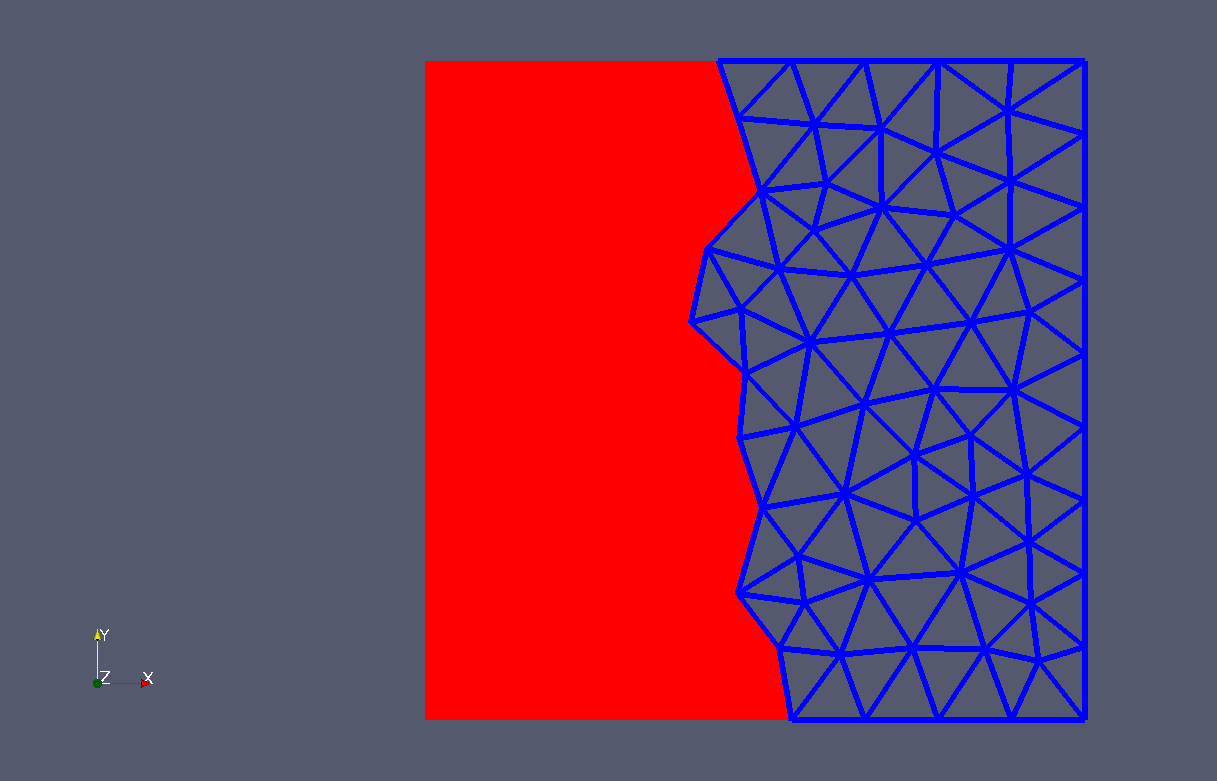
\includegraphics[width=.7\linewidth]{mymeshpartition}
%\label{fig:1}
%\caption{Screenshot of Paraview (3.2.1) of a 2D mesh partitioned and distributed on two processors}
%\end{figure}
\subsection{Examples}
\label{mesh:examples}
Here is an example of how to get a simplex or hypercube geometry :

\lstinputlisting[linerange=marker4-endmarker4]{mymesh.cpp}
The parameter \lstinline!_h! in the function \lstinline!domain! allows to change the mesh characteristic size to \lstinline!M_meshsize! which is given for example on the command-line using the Application framework, please refer to ~\ref{sec:creat-appl} for more details. You can see the meshes, by executing with the followings ordering :

\begin{unixcom}
		./feel_doc_mymesh --shape=simplex
		./feel_doc_mymesh --shape=hypercube
\end{unixcom}
we generate some of the following graphics (which are located in \verb|~/feel/doc/tutorial/mymesh/| \newline \verb|hypercube-x/h_y.z| or \verb|~/feel/doc/tutorial/mymesh/simplex-x/h_y.z|)
\begin{figure}[!h]
\begin{minipage}[b]{.50\linewidth}
\centering

\includegraphics[width=4.5cm]{pngs/mymesh/hypercube_1.png}
\caption{Line in 1D}
\end{minipage}
\begin{minipage}[b]{.50\linewidth}
\centering
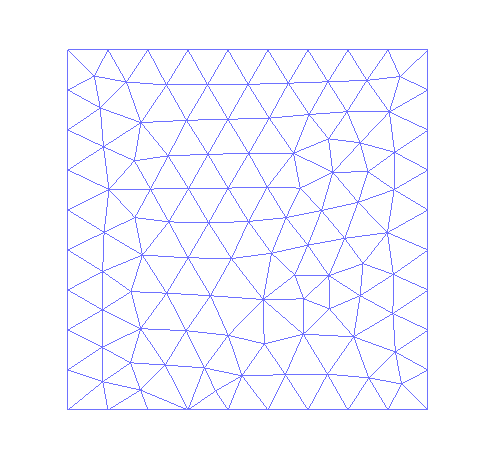
\includegraphics[width=4.5cm]{pngs/mymesh/hypercube_2.png}
\caption{Cube in 2D}
\end{minipage}
\label{fig.erreur}
\end{figure}
\newline
\begin{figure}[!h]
\begin{minipage}[b]{.50\linewidth}
\centering
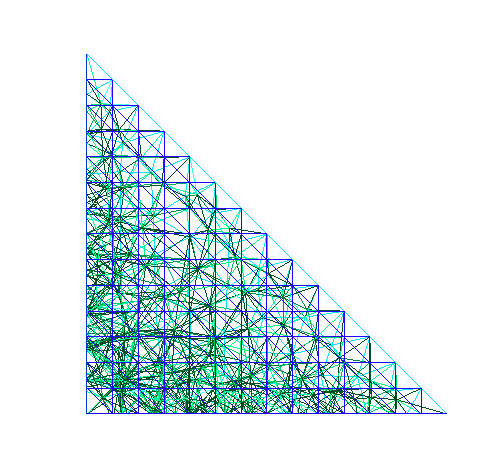
\includegraphics[width=4.5cm]{pngs/mymesh/simplex_3.png}
\caption{Tetrahedron}
\end{minipage}
\begin{minipage}[b]{.50\linewidth}
\centering
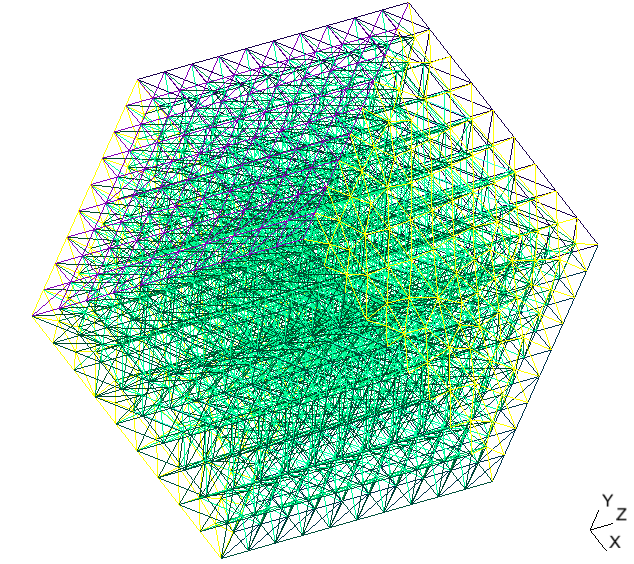
\includegraphics[width=4.5cm]{pngs/mymesh/hypercube_3.png}
\caption{Unit cube in 3D}
\end{minipage}
\end{figure}

%\begin{centering}
%\begin{tabular}{cc}
%
\includegraphics[width=4.5cm]{pngs/mymesh/hypercube_1.png} %\caption{Line in 1D}
%&
%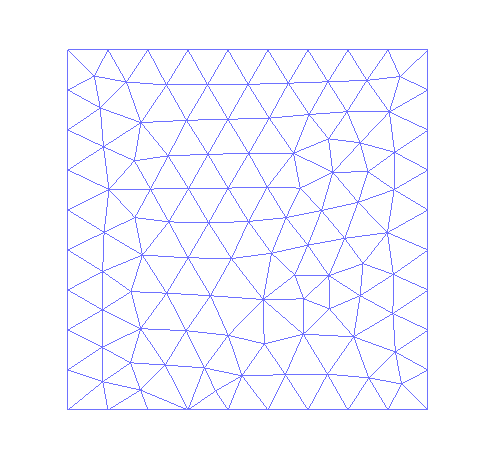
\includegraphics[width=4.5cm]{pngs/mymesh/hypercube_2.png} %\caption{Cube in 2D}
% \\
%\verb|Line in 1D| & \verb|Cube in 2D|
%\\
%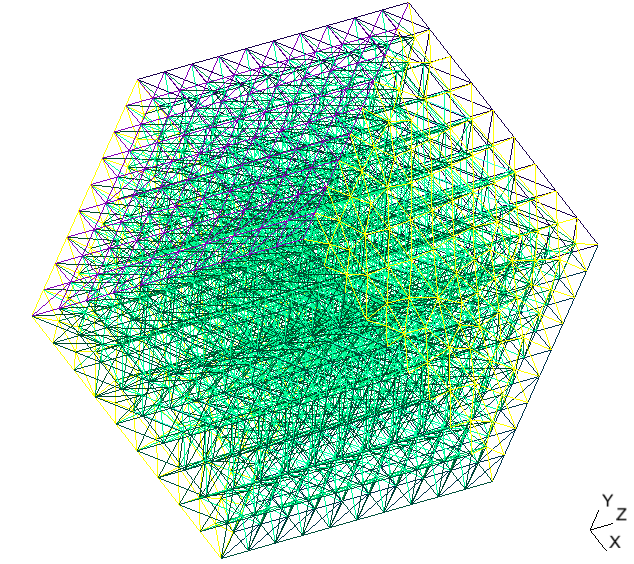
\includegraphics[width=4.5cm]{pngs/mymesh/hypercube_3.png} %\caption{Unit cube in 3D}
%&
%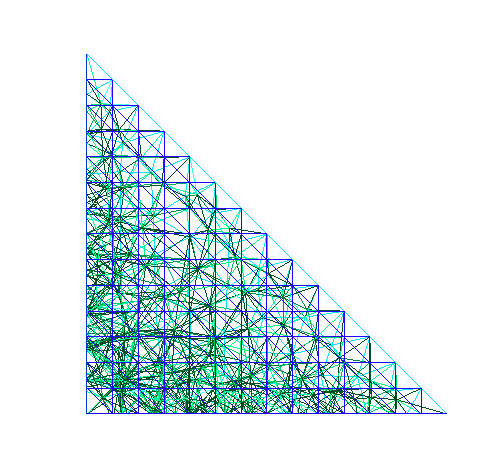
\includegraphics[width=4.5cm]{pngs/mymesh/simplex_3.png} %\caption{Tetrahedron}
%\\
%\verb|Unit cube in 3D| & \verb|Tetrahedron|
%\end{tabular}
%\end{centering}
To admire the meshes you've generated, you should go to \lstinline!~/feel/doc/tutorial/mymesh/hypercube! (or \lstinline!simplex!) and find out the \verb|.msh| files. Last step is to launch gmsh with
\begin{unixcom}
		gmsh yourfile.msh
\end{unixcom}

\subsection{Exporting meshes for post-processing}

We can export the mesh to two postprocessing formats supported at the moment :
\begin{itemize}
\item \textbf{Ensight} (sos and case)  which is supported by the software Ensight and Paraview;
\item \textbf{Gmsh} which is post-processing format of Gmsh.
\end{itemize}

We define the exporter data structure type as follows :
\lstinputlisting[linerange=marker61-endmarker61]{mymesh.cpp}

By default, the  export format is ensight. We can use the code \lstinline!Exporter::setMesh()! and \lstinline!Exporter::save()! to save the mesh to the format given to the command line --exporter= <format>

\lstinputlisting[linerange=marker62-endmarker62]{mymesh.cpp}

To take into account the exporting format, you have to type thoses syntaxes
\begin{unixcom}
		./feel_doc_mymesh  --exporter= gmsh
		./feel_doc_mymesh  --exporter= paraview
\end{unixcom}


\subsection{Iterating over the entities of a mesh}

\feel mesh data structures provides powerful iterators that allows to
walk though the mesh in various ways: iterate over element, faces ,
points, marked\footnote{associated to an integer flag denoting a
  region, material, processor} elements, marked faces, ...

\section{Computing integrals}
\label{sec:computing-integrals}
\marginpar{\lstinline!myintegrals.cpp!}

\subsection{Problem statement}

If you have followed this tutorial in the order, you are now able to create a simple application and generate meshes. We are now interested in computing integrals on the meshes we have generated. Let's consider this mesh (no matter which one) on a domain $\Omega$ and parts of the domain, i.e. subregions and (parts of) boundary. In this tutorial the domain can be either

\[ \Omega=[0,1]^d\ \subset\ \mathbb{R}^d \]

or

\[ \Omega=\{ \mathbf{x} \in \mathbb{R}^d | x_i \geq 0, \sum_{i=1}^{d} x_i \leq 1 \} \]

where $ d=1,2$ or $3$ and $\mathbf{x}=(x_1,...,x_d)$.\\ \newline
These domains are plotted in the section ~\ref{sec:mesh-manipulation} (If it's not yet done, compile all examples which are used in this tutorial, go to \lstinline!~/FEEL/feel.opt/doc/manual/! and type \verb|make| and execute the application \verb|feel_doc_mymesh|). The execution will result in several meshes as it is explained in ~\ref{mesh:examples}.\\
Here are the integrals we want to compute :
\begin{itemize}
\item $\displaystyle{ \int_\Omega 1 }$ : the measure of the domain
\item $\displaystyle{ \int_{\partial\Omega} 1 }$: the measure of the surface of the domain (Dim>1)
\item $ \displaystyle{\int_{\Omega} x^2+y^2+z^2 }$ : the integral over $\displaystyle{\Omega}$ of $ \displaystyle{(x,y,z) \mapsto x^2+y^2+z^2}$ with the convention that $y=z=0$ in 1D and $ z=0 $ in 2D.
\item $\displaystyle{ \int_{\Omega} sin(x^2+y^2+z^2)} $ : the integral over $\Omega$ of $\displaystyle{ (x,y,z) \mapsto sin(x^2+y^2+z^2)}$ with the same convention as above.
\end{itemize}

\subsection{Implementation}

To compute an integral, we use the following function
\begin{lstlisting}
integrate( <domain>,<expression under the integral> ).evaluate(<location>)
\end{lstlisting}

\subsubsection{Domain}

You have to indicate the domain on which we want to integrate. It consists in a pair of iterators over the elements owned by the current processor (the mesh is shared between the processors).
\begin{itemize}
\item To compute the integral over the region of $\Omega$ current processor, use
\begin{lstlisting}
elements(mesh)
\end{lstlisting}
\item To compute the integral on the boundary faces of the domain $\Omega$, use
\begin{lstlisting}
boundaryfaces(mesh)
\end{lstlisting}
\end{itemize}

\subsubsection{Expression under the integrals}

The language provided by \feel (called the Finite Element Embedded Language) brings the keyword $Px()$, $Py()$ and $Pz()$ to denote the $x$, $y$ and $z$ coordinates. \\
The expression $x^2 + y^2 + z^2$ under the third integral should be written such as :
\begin{lstlisting}
Px()*Px() + Py()*Py() + Pz()*Pz()
\end{lstlisting}
\vspace{0.2cm}
The constants are indicated by the function constant() (for example, we have to indicate \lstinline!constant(1.0)! for the first integral). \\

\subsubsection{Examples}

\paragraph{First integral : domain area \\}
To compute the first integral (the domain area), the code reads :
\lstinputlisting[linerange=marker1-endmarker1]{myintegrals.cpp}


This compute the integral only on the region of the domain owned by the current processor \lstinline!(local_domain_area)!. \\

To obtain the total area, we collect the integrals on all processors using a reduce MPI operation and sum all contributions. We have used here the \lstinline!Boost.MPI! library that provides an extremely powerful wrapper around the MPI library. \\
\lstinputlisting[linerange=marker2-endmarker2]{myintegrals.cpp}

\vspace{0.2cm}
Finally, we print to the log file the result of the local and global integral calculation.
\lstinputlisting[linerange=marker3-endmarker3]{myintegrals.cpp}

\paragraph{Second integral : domain perimeter \\}

The difference with the domain area computation resides in the elements with are iterating on: here we are iterating on the boundary faces of the domain to compute the integral using \lstinline!boundaryfaces(mesh)! to provide the pairs of iterators. But the stages are the same as previously \\

\lstinputlisting[linerange=marker4-endmarker4]{myintegrals.cpp}

We can apply the same method to compute the third, and the last integral. \\

\subsection{Quadrature}

Feel computes automatically the quadrature associated to the expression under the integral. If the expression is polynomial then the quadrature is exact. If the expression is not polynomial, then each non-polynomial term in the expression is considered as a polynomial of degree 2 by default.

Here is how the 4-th integral can be computed letting Feel decide about the quadrature \\
\lstinputlisting[linerange=marker6-endmarker6]{myintegrals.cpp}

An alternative is to set yourself the quadrature by passing a new argument to the integrate function: \_Q<Order>() where Order is the maximum polynomial order that the quadrature should integrate exactely.
\lstinputlisting[linerange=marker7-endmarker7]{myintegrals.cpp}

\subsection{Complete example : application, mesh and integrals}

Here, we'll see how to build an application which create a mesh, and compute some integrals on it.

\subsubsection{Application building}
As we can see in the creating applications section (~\ref{sec:creat-appl}), we can add a description and some options to our new application.
Here, we have created two functions \lstinline!makeAbout()! and \lstinline!makeOptions()! which create respectively the descritpion and the list of options.
\lstinline!makeOptions()! creates a list of options (myintegralsoptions), and adds two options :
\begin{itemize}
\item \lstinline!hsize! which corresponds to the mesh size (default = $0.2$)
\item \lstinline!shape! which corresponds to the shape of the domain (default = $hypercube$)
\end{itemize}

\lstinputlisting[linerange=marker8-endmarker8]{myintegrals.cpp}

makeAbout() gives the description of the application :\\

\lstinputlisting[linerange=marker9-endmarker9]{myintegrals.cpp}

To get further information about the application, see creating applications section ~\ref{sec:creat-appl}.

\subsubsection{Class definition}

Once the description and options have been defined, we create the class Myintegrals, with the constructor \\
\begin{lstlisting}
MyIntegrals( po::variables_map const& vm, AboutData const& about )
\end{lstlisting}
which takes \lstinline!vm! (a map which associates the available options with their default value), and \lstinline!about! (containing our application's description). \\

The \lstinline!run()! member function is redifined twice in this class :
\lstinputlisting[linerange=marker10-endmarker10]{myintegrals.cpp}
These two versions are linked, because the first uses the second. Indeed, \lstinline!run()! stores the parameters we have chosen with the options \lstinline!(mesh size, shape, $\dots$)!, and uses them in the second version (X corresponds to these parameters : \lstinline!X[0]=mesh_size! and \lstinline!X[1]=mesh_shape!). \\

\subsubsection{The run() member function}
In this function, we create a subdirectory of feel in which there will be the results of our application, and logfiles containing :
\begin{itemize}
\item the application's name
\item the mesh size
\item the mesh shape
\end{itemize}

\begin{lstlisting}
if ( !this->vm().count( "nochdir" ) )
Environment::changeRepository( boost::format( "doc/tutorial/%1%/%2%/h_%3%/")
                                  this->about().appName()
                                  shape
                                  meshSize );

\end{lstlisting}

It is also in run() that we create the mesh before to compute the integrals :
\lstinputlisting[linerange=marker11-endmarker11]{myintegrals.cpp}
Now that we have a computational mesh, we can compute the integrals as we have seen before :

\begin{lstlisting}
    double local_domain_area = integrate( elements(mesh),
                                        constant(1.0)).evaluate()(0,0);

    double global_domain_area=local_domain_area;
    if ( this->comm().size()  > 1 )
        mpi::all_reduce( this->comm(),
                         local_domain_area,
                         global_domain_area,
                         std::plus<double>() );

    Log() << "int_Omega 1 = " << global_domain_area
          << "[ " << local_domain_area << " ]\n";
\end{lstlisting}

\subsection{Results}

After compiling \lstinline!feel_doc_myintegrals! with the defaults options
\begin{lstlisting}
  --hsize arg (=0.20000000000000001)    mesh size
  --shape arg (=hypercube)              shape of the domain
\end{lstlisting}

we obtain the values of each integrals, in each dimension ($1,2$ and $3$) : \\
\begin{lstlisting}
------------------------------------------------------------
Execute MyIntegrals<1>
int_Omega 1 = 1[ 1 ]
int_Omega (x^2+y^2+z^2) = 0.333333[ 0.333333 ]
int_Omega (sin(x^2+y^2+z^2)) [with order 4 max exact integration]= 0.310268[ 0.310268 ]
int_Omega (sin(x^2+y^2+z^2)) [with order 2 max exact integration] = 0.310281[ 0.310281 ]
------------------------------------------------------------
Execute MyIntegrals<2>
int_Omega 1 = 1[ 1 ]
int_BoundaryOmega (1)= 4[ 4 ]
int_Omega (x^2+y^2+z^2) = 0.666667[ 0.666667 ]
int_Omega (sin(x^2+y^2+z^2)) [with order 4 max exact integration]= 0.56129[ 0.56129 ]
int_Omega (sin(x^2+y^2+z^2)) [with order 2 max exact integration] = 0.561299[ 0.561299 ]
------------------------------------------------------------
Execute MyIntegrals<3>
int_Omega 1 = 1[ 1 ]
int_BoundaryOmega (1)= 6[ 6 ]
int_Omega (x^2+y^2+z^2) = 1[ 1 ]
int_Omega (sin(x^2+y^2+z^2)) [with order 4 max exact integration]= 0.731683[ 0.731683 ]
int_Omega (sin(x^2+y^2+z^2)) [with order 2 max exact integration] = 0.731693[ 0.731693 ]
\end{lstlisting}



\section{Function Spaces}
\marginpar{\lstinline!myfunctionspace.cpp!}
\label{sec:func-spaces}

\subsection{Functions spaces definition}

In order to resolve partial derivative equations, we have to define the function space on which we work.
We can define a new type \lstinline!space_type! which corresponds to our new functions space
\begin{lstlisting}
 typedef FunctionSpace<mesh_type, basis_type> space_type;
\end{lstlisting}
To define this function space, we have to define :
\begin{itemize}
 \item \lstinline!mesh_type! the mesh on which we work (see~\ref{sec:mesh-manipulation})
 \item \lstinline!basis_type! the base of the function space (see~\ref{sec:base-funct})
\end{itemize}

\underline{Remark} : We can use the librairie Boost.smartptr of Boost, which has a reference counter (in the shared\_ptr class). It permits
to manage the memory (If we have built an object and that there are no more any pointers on it, it is automatically destructed.)

\subsubsection{Base of the function space}
\label{sec:base-funct}
To define the base of functions we want to use, we have to indicate :
\begin{itemize}
 \item The type of the polynoms ($\mathbb{P}$) we want to use
 \begin{itemize}
   \item Lagrange (more used than the others because more customizable)
   \item Legendre (only for hypercube)
   \item Dubiner (only for simplex)
   \item Crouzeix-Raviart
   \item Raviart-Thomas
 \end{itemize}

 \item The order of these polynoms (an integer in $\mathbb{N}^*$)
 \item The dimension of Im(P) (\lstinline!Scalar! if Im($\mathbb{P})=\mathbb{R}$, \lstinline!Vectorial! if the dimension is up to $1$)
 \item The continuity of polynoms at the interface ( \lstinline!Continuous! or \lstinline!Discontinuous!)
\end{itemize}
After we have chosen this parameters, we can create the new function base (new type \lstinline!basis_type!) :
\begin{lstlisting}
 typedef bases<Lagrange<0,Scalar,Discontinuous> > basis_type;
\end{lstlisting}

Here, we build a base with Lagrange polynoms, with order 0. The result of these polynoms is a scalar, and we authorized them
to be discontinue at the interface between two elements. In our example, \lstinline!p0_space_type! is the function space that holds piecwise constant $\mathbb{P}_0$ functions :  \\
\lstinputlisting[linerange=marker1-endmarker1]{myfunctionspace.cpp}

\subsubsection{Instantiation of the function space}

We want now to instanciate the function space $X_h$ of type \lstinline!space_type! (that we created previously). \\

First, we build the mesh on which we want to work (of type \lstinline!mesh_ptrtype!)
\lstinputlisting[linerange=marker31-endmarker31]{myfunctionspace.cpp}

Then we instantiate $X_h$ using \lstinline!space_type::New()! static member function and obtain a \lstinline!space_ptrtype!.
\lstinputlisting[linerange=marker32-endmarker32]{myfunctionspace.cpp}
We are now able to instanciate elements on $X_h$. There are two ways to proceed, using auto keyword allowing to infer automatically the type of $ X_h$ elements or knowing the actual type of the elements
\lstinputlisting[linerange=marker33-endmarker33]{myfunctionspace.cpp}

\subsection{Using function space and functions}
\subsubsection{Projection}

First, we define some mathematical expression/functions

\begin{eqnarray*}
g(x,y,z) &=& \sin(\pi x/2)\ \cos(\pi y/2)\ \cos(\pi*z/2) \\
f(x,y,z) &=& (1-x^2)\ (1-y^2)\ (1-z^2)\ (x^2+y^2+z^2)^{\alpha/2.0},\quad \alpha=3
\end{eqnarray*}
In our example, these functions correspond to 
\lstinputlisting[linerange=marker4-endmarker4]{myfunctionspace.cpp}
(they are implemented using the new auto C++ keyword to infer the type of expression automatically). \\ \\
Then we build the interpolant (Lagrange interpolant in this case since we chose Lagrange basis function), by calling the \lstinline!vf::project()! function which can be applied on all or parts of the mesh thanks to the mesh iterators such as \lstinline!elements(mesh)! or \lstinline!markedelements(mesh,marker)!.
The return object is the interpolant of the function in the space $ X_h $ given as an argument to \lstinline!vf::project()!.
\lstinputlisting[linerange=marker5-endmarker5]{myfunctionspace.cpp}
Here, $u$ is the projection of $g$ on the nodes of the mesh. Note that $u$ and $g$ have not the same type. To evaluate the error of $(u-g)$ on the nodes, we have to evaluate the function $u$, with the function $v$.

\subsubsection{Norm}

To calculate norms, we use integrals. For example, the $L_2$ norm is defined by :
$$\displaystyle{\| g\|_{L_2} = \sqrt{\int_\varOmega (g)^2}}$$
To compute this, we use the integrate function (See ~\ref{sec:computing-integrals}) with \lstinline!elements(mesh)! which allows to integrate on the entire domain.
Let's see an example of norms computation with log file printing :
\lstinputlisting[linerange=marker6-endmarker6]{myfunctionspace.cpp}


\subsection{Results}

\subsubsection{Execution without option}

We have made a test code (it is still \verb|myfunctionspace.cpp| which create a new application myfunctionspace with some options (added with a \lstinline!makeOptions()! function),
and a description (with a \lstinline!makeAbout()! function). (See~\ref{sec:creat-appl}). \\

This code applies the examples we have seen previously, and when we execute it without option, we obtain :

\begin{lstlisting}
Execute MyFunctionSpace<2>
||u-g||_0=0.00463274
||v-f||_0=0.000483591
---------------------------------------------------
Execute MyFunctionSpace<3>
||u-g||_0=0.00968019
||v-f||_0=0.000474499
\end{lstlisting}
As we have seen before, $u$ is the projection of $g$ in the function space. So on the mesh nodes, the error's norm has to be
zero (the results we obtain here don't seems to be coherent).


%\subsection{Using functions spaces and functions}

%\begin{itemize}
%\item interpolating
%\item nodal projection
%\item saving
%\end{itemize}


\section{Linear Algebra}
\label{sec:linear-algebra}


\feel supports three different linear algebra environments that we
shall call \emph{backends}.
\begin{itemize}
\item Gmm\footnote{}
\item Petsc\footnote{}
\item Trilinos\footnote{}
\end{itemize}


\subsection{Choosing a linear algebra backend}
\label{sec:choos-line-algebra}

\index{Class!Backend}\index{boost!shared\_ptr}
To select a backend in order to solve a linear system, we instantiate
the \lstinline!Backend! class associated.

\begin{lstlisting}
#include <feel/feelalg/backend.hpp>
boost::shared_ptr<Backend<double> > backend =
     Backend<double>::build( BACKEND_PETSC );
\end{lstlisting}

The backend provides an interface to solve
\begin{equation}
  \label{eq:8}
  A x = b
\end{equation}
\noindent
where $A$ is a $n \times n $ sparse matrix and $x,b$ vectors of size $n$.
The backend defines the \cpp types for  each of these, e.g.
\begin{lstlisting}
Backend<double>::sparse_matrix_type A;
Backend<double>::vector_type x,b;
\end{lstlisting}
\noindent
In practice, we use the \lstinline!boost::shared_ptr<>! shared pointer
to ensure that we won't get memory leaks. The backends provide a
corresponding \lstinline!typedef!


\begin{lstlisting}
Backend<double>::sparse_matrix_ptrtype A( backend->newMatrix( Xh, Yh ) );
Backend<double>::vector_ptrtype x( backend->newVector( Yh ) );
Backend<double>::vector_ptrtype b( backend->newVector( Xh ) );
\end{lstlisting}
\noindent
where $X_h$ and $Y_h$ are function spaces providing the number of
degrees of freedom that will define the size of the matrix and vectors
thanks to the helpers functions \lstinline!Backend::newMatrix()! and
\lstinline!Backend::newVector!. In a parallel setting, the
local/global processor mapping would be passed down by the function
spaces.

\subsection{Defining and using matrices and vectors}
\label{sec:defin-using-matr}

\subsection{Solving}
\label{sec:solving}


\section{Variational Formulation}
\label{sec:vari-form}

\index{formulation!variational}
\begin{itemize}
\item keywords
\item principles
\end{itemize}

\subsection{Computing integrals}
\label{sec:computing-integrals}

\index{integrals}
\marginpar{\lstinline!myintegrals.cpp!}
We would like to compute some integrals on a domain of $\Omega=[0,1]^d\ \subset\ \mathbb{R}^d$
and parts of the domain, i.e. subregions and (parts of) boundary.

Once we have defined the computational mesh, we would like to compute
the area of the domain. We form the integral $\int_\Omega 1$, the code
reads as follows

\lstinputlisting[linerange=marker1-endmarker1]{myintegrals.cpp}

\lstinline!elements(mesh)! returns a pair of iterators over the
elements owned by the current processor, \lstinline!im! is an instance
of the \lstinline!im_type! which provides a quadrature method to
integrate exactly polynomials up to degree 2. In our case integrating
constant(degree 0) would have sufficed, but we will reuse
\lstinline!im! later. Now that we have computed the integral of 1 over
the region of $\Omega$ current processor (ie the area of the domain
owned by the processor), we want to compute the area of $\Omega$. To
do that we collect the integrals on all processors using a
\lstinline!reduce! MPI operation and sum all contributions. We have
used here the Boost.MPI library that provides an extremely powerful
\cpp wrapper around the MPI library. The code reads

\lstinputlisting[linerange=marker2-endmarker2]{myintegrals.cpp}

\noindent
Finally, we print to the log file the result of the local and global
integral calculation. Another calculation is for example to compute
the perimeter of the domain

\lstinputlisting[linerange=marker3-endmarker3]{myintegrals.cpp}

\noindent
the main difference with the domain area computation resides in the
elements with are iterating on: here we are iterating on the boundary
faces of the domain to compute the integral using
\lstinline!boundaryfaces(mesh)! to provide the pairs of iterators.


Now say that we want to compute
\begin{equation}
  \label{eq:5}
  \int_\Omega x^2 + y^2 dx dy.
\end{equation}
The Finite Element Embedded Language (FEEL++) language provides the
keyword \lstinline!Px()! and \lstinline!Py()! to denote the $x$ and
$y$ coordinates like in equation~(\ref{eq:5}).  The code reads then


\lstinputlisting[linerange=marker4-endmarker4]{myintegrals.cpp}

Note that in this case, we really require the use of a quadrature that
integrates exactly order 2 polynomials.

Let's run now the tutrial example \lstinline!myintegrals!. The results are stored
in the log file under \lstinline!~/feel/myintegrals/!.

\begin{lstlisting}{language=sh}
> cat ~/feel/myintegrals/Simplex_2_1/h_0.5/myintegrals-1.0
myintegrals-1.0 is opened for debug
[Area 0] int_Omega = 1[ 1 ]
[Area 0] int_Omega = 4[ 4 ]
[Area 0] int_Omega = 0.666667[ 0.666667 ]
\end{lstlisting}

We remark that the results are exact. Integrating higher order
polynomials ($\geq 3$) or non-polynomial function would typically
require higher order quadrature to get accurate results. To do that
increase \lstinline!imOrder! in the example and try integrating
$f(x,y)=x^3 + x y^2$.


In order to see what happens in parallel, use \lstinline!mpirun! to
launch \lstinline!myintegrals! on several processors, for example

\begin{lstlisting}{language=sh}
> mpirun -np 4 myintegrals --hsize=0.1
> cat ~/feel/myintegrals/Simplex_2_1/h_0.1/myintegrals-4.0
myintegrals-4.0 is opened for debug
[Area 0] int_Omega = 1[ 0.253348 ]
[Area 0] int_Omega = 4[ 1.44444 ]
[Area 0] int_Omega = 0.666667[ 0.0701812 ]
> cat ~/feel/myintegrals/Simplex_2_1/h_0.1/myintegrals-4.1
myintegrals-4.1 is opened for debug
[Area 0] int_Omega = 1[ 0.288919 ]
[Area 0] int_Omega = 4[ 0.444444 ]
[Area 0] int_Omega = 0.666667[ 0.186251 ]
> cat ~/feel/myintegrals/Simplex_2_1/h_0.1/myintegrals-4.2
myintegrals-4.2 is opened for debug
[Area 0] int_Omega = 1[ 0.183219 ]
[Area 0] int_Omega = 4[ 1.11111 ]
[Area 0] int_Omega = 0.666667[ 0.105008 ]
> cat ~/feel/myintegrals/Simplex_2_1/h_0.1/myintegrals-4.3
myintegrals-4.3 is opened for debug
[Area 0] int_Omega = 1[ 0.274514 ]
[Area 0] int_Omega = 4[ 1 ]
[Area 0] int_Omega = 0.666667[ 0.305227 ]
\end{lstlisting}

\subsection{Standard formulation: the Laplacian case}
\label{sec:defin-bilin-forms}
\index{laplacian}
\subsubsection{Mathematical formulation}
\label{sec:math-form-3}
\index{laplacian!formulation!mathematical}
\marginpar{\lstinline!laplacian.cpp!}
In this example, we would like to solve for the following problem in 2D
\begin{problem}
\label{prob:1}
 find $u$ such that
\begin{equation}
  \label{eq:1}
  -\Delta u = f\ \text{in}\ \Omega = [-1;1]^2
\end{equation}
with
\begin{equation}
  \label{eq:2}
  f= 2 \pi^2  g
\end{equation}
and $g$ is the exact solution
\begin{equation}
  \label{eq:3}
  g=\sin(\pi x) \cos(\pi y)
\end{equation}
The following boundary conditions apply
\begin{equation}
  \label{eq:4}
  u=g_{|x=\pm 1}, \quad \frac{\partial u}{\partial n} = 0_{|y=\pm 1}
\end{equation}
\end{problem}

We propose here two possible variational formulations. The first one,
handles the Dirichlet boundary conditions strongly, that is to say the
condition is \emph{incorporated} into the function space definitions.
The second one handles the Dirichlet condition \emph{weakly} and hence
we have a uniform treatment for all types of boundary conditions.



\paragraph{Strong Dirichlet conditions}
\label{sec:strong-dirichl-cond}

\noindent
The variational formulation reads as follows, we introduce the spaces
\begin{equation}
  \label{eq:11}
  \mathcal{X} = \Big\{ v \in H_1(\Omega) \text{ such that } v=g_{|x=-1,x=1} \Big\}
\end{equation}
and
\begin{equation}
  \label{eq:12}
  \mathcal{V} = \Big\{ v \in H_1(\Omega) \text{ such that } v=0_{|x=-1,x=1} \Big\}
\end{equation}
We multiply (\ref{eq:1}) by $v \in \mathcal{V}$ then integrate over $\Omega$ and obtain
\begin{equation}
  \label{eq:13}
  \int_\Omega -\Delta u v = \int_\Omega f v
\end{equation}
We integrate by parts and reformulate the problem as follows:
\begin{problem}
we look
for $u \in \mathcal{X}$ such that for all $v \in \mathcal{V}$
\begin{equation}
  \label{eq:14}
  \int_\Omega \nabla u \cdot \nabla v  = \int_\Omega f v
\end{equation}

\end{problem}
In the present space setting~(\ref{eq:12}) and boundary
conditions~(\ref{eq:4}), we have the boundary term from the integration by
parts which is dropped being equal to 0
\begin{equation}
  \label{eq:15}
  \int_{\partial \Omega} \frac{\partial u}{\partial n} v = 0,
\end{equation}
recalling that
\begin{equation}
  \label{eq:21}
  \frac{\partial u}{\partial n} \stackrel{\text{def}}{=} \nabla u \cdot n
\end{equation}
where $n$ is the outward normal to $\partial \Omega$ by convention.We
now discretize the problem, we create a mesh out of $\Omega$, we have
\begin{equation}
  \label{eq:10}
  \Omega = \cup_{e=1}^\nel \Omega^e
\end{equation}
where $\Omega^e$ can be segments, triangles or tetrahedra depending on
$d$ and we have $\nel$ of them. We introduce the finite dimensional
spaces of continuous piecewise polynomial of degree $N$ functions
\begin{equation}
  \label{eq:17}
  X_h = \Big\{ v_h  \in C^0(\Omega),\ {v_h}_{|\Omega^e} \in \mathbb{P}_N( \Omega^e ),\   v_h=g_{|x=-1,x=1}\Big\}
\end{equation}
and
\begin{equation}
  \label{eq:18}
  V_h = \Big\{ v_h \in C^0(\Omega),\ {v_h}_{|\Omega^e} \in \mathbb{P}_N( \Omega^e ),\   v_h=0_{|x=-1,x=1}\Big\}
\end{equation}
which are out trial and test function spaces respectively.  We now
have the problem we seek to solve which reads in our continuous
Galerkin framework
\begin{problem}
  \label{prob:2}
  we look for $u_h \in X_h \subset \mathcal{X}$ such that for all $v
  \in V_h \subset \mathcal{V}$
  \begin{equation}
    \label{eq:20}
    \int_\Omega \nabla u_h \cdot \nabla v_h  = \int_\Omega f v_h
  \end{equation}
\end{problem}

\paragraph{Weak Dirichlet conditions}
\label{sec:weak-dirichl-cond}

There is an alternative formulation which allows to treat weakly
Dirichlet(Essential) boundary conditions similarly to Neumann(Natural)
and Robin conditions. Following a similar development as in the previous section, the problem reads
\begin{problem}
  \label{prob:3}
  we look for $u \in X_h \subset H_1(\Omega)$ such that for all $v \in
  X_h$
\begin{equation}
  \label{eq:16}
  \int_\Omega \nabla u \cdot \nabla v +
  \int_{|x=-1,x=1} -\frac{\partial u}{\partial n} v - u \frac{\partial v}{\partial n} + \frac{\mu}{h} u v
  =
  \int_\Omega f v +
  \int_{|x=-1,x=1}  - g \frac{\partial v}{\partial n} + \frac{\mu}{h} g v
\end{equation}
where
\begin{equation}
  \label{eq:19}
  X_h = \Big\{ v_h \in C^0(\Omega),\ {v_h}_{|\Omega^e} \in \mathbb{P}_N( \Omega^e ) \Big\}
\end{equation}
\end{problem}
In (\ref{eq:16}), $g$ is defined by (\ref{eq:3}). $\mu$ serves as a penalisation
parameter which should be $> 0$, e.g. between 2 and 10, and $h$ is the
size of the face. The inconvenient of this formulation is the
introduction of the parameter $\mu$, but the advantage is the
\emph{weak} treatment of the Dirichlet condition.

\subsubsection{Feel formulation}
\label{sec:feel-formulation-1}

\index{laplacian!formulation!feel}
First we define the $f$ and $g$. To do that we use the
\lstinline!AUTO! keyword and associate to \lstinline!f! and
\lstinline!g! their expressions

\lstinputlisting[linerange=marker1-endmarker1]{laplacian.cpp}

\noindent where \lstinline!M_PI! is defined in the header
\lstinline!cmath!.  Using \lstinline!AUTO! allows to defined
\lstinline!f!  and \lstinline!g! --- which are moderately complex
object --- without having to know the actual type. \lstinline!AUTO!
determines automatically the type of the expression using the
\lstinline!__typeof__! keyword internally.

Then we form the right hand side by defining a linear form whose
algebraic representation will be stored in a
\lstinline!vector_ptrtype! which is provided by the chosen linear
algebra backend. The linear form is equated with an integral
expression defining our right hand side.

\lstinputlisting[linerange=marker2-endmarker2]{laplacian.cpp}

\noindent \lstinline!form1! generates an instance of the object
representing linear forms, that is to say it mimics the mathematical
object $\ell$ such that
\begin{equation}
  \label{eq:9}
  \begin{array}{rccl}
    \ell: & X_h & \mapsto & \mathbb{R}\\
    & v_h & \rightarrow &\ell(v_h)=\int_\Omega f v
  \end{array}
\end{equation}
which is represented algebraically in the code by the vector
\lstinline!F! using the argument \lstinline!_vector!. The last
argument \lstinline!_init!, if set to \lstinline!true!\footnote{It is
  set to \lstinline!false! by default.}, will zero-out the entries of
the vector \lstinline!F!.


We now turn to the left hand side and define the bilinear form using
the \lstinline!form2! helper function which is passed \textit{(i)} the
trial function space using the \lstinline!_trial! option,
\textit{(ii)} the test function space using the \lstinline!_test!
option, \textit{(iii)} the algebraic representation using
\lstinline!_matrix!, i.e. a sparse matrix whose type is derived from
one of the linear algebra backends and \textit{(iv)} whether the
associated matrix should initialized using
\lstinline!_init!.


\lstinputlisting[linerange=marker3-endmarker3]{laplacian.cpp}


Finally, we deal with the boundary condition, we implement both
formulation described in appendix~\ref{sec:vari-form-1}. For a
\emph{strong} treatment of the Dirichlet condition, we use the
\lstinline!on()! keyword of FEEL++ as follows

\lstinputlisting[linerange=marker5-endmarker5]{laplacian.cpp}

Notice that we add, using \lstinline!+=!, the Dirichlet contribution
for the bilinear form. The first argument is the set of boundary faces
to apply the condition: in gmsh the points satisfying $x=\pm 1$ are
marked using the flags $1$ and $3$ ($x=-1$ and $x=1$ respectively.)

To implement the weak Dirichlet boundary condition, we add the
following contributions to the left and right hand side:

\lstinputlisting[linerange=marker41-endmarker41]{laplacian.cpp}
\lstinputlisting[linerange=marker4-endmarker4]{laplacian.cpp}

Note that we use the command line option \lstinline!--weakdir! set to
1 by default to decide between weak/strong Dirichlet handling.  Apart
the uniform treatment of boundary conditions, the weak Dirichlet
formulation has the advantage to work also in a parallel environment.

Next we solve the linear system
\begin{equation}
  \label{eq:6}
  D u = F
\end{equation}

where the \lstinline!solve! function is implemented as follows

\lstinputlisting[linerange=marker6-endmarker6]{laplacian.cpp}

Finally we check for the $L_2$ error in our approximation by computing
\begin{equation}
  \label{eq:7}
  \|u-u_h\|_{L_2}\ =\ \sqrt{\int_\Omega (u-u_h)^2} = \sqrt{\int_\Omega (g-u_h)^2}
\end{equation}
where $u$ is the exact solution and is equal to $g$ and $u_h$ is the
numerical solution of the problem~(\ref{eq:1}) and the components of
$u_h$ in the $P_2$ Lagrange basis are given by solving (\ref{eq:6}).

The code reads

\lstinputlisting[linerange=marker7-endmarker7]{laplacian.cpp}


You can now verify that the $L_2$ error norm behaves like $h^{-(N+1)}$
where $h$ is the mesh size and $N$ the polynomial order. The $H_1$
error norm would be checked similarly in $h^{-N}$. The
figure~\ref{fig:2} displays the results using Paraview.

\begin{figure}[htbp]
  \centering
  \subfigure[Colored with $u$]{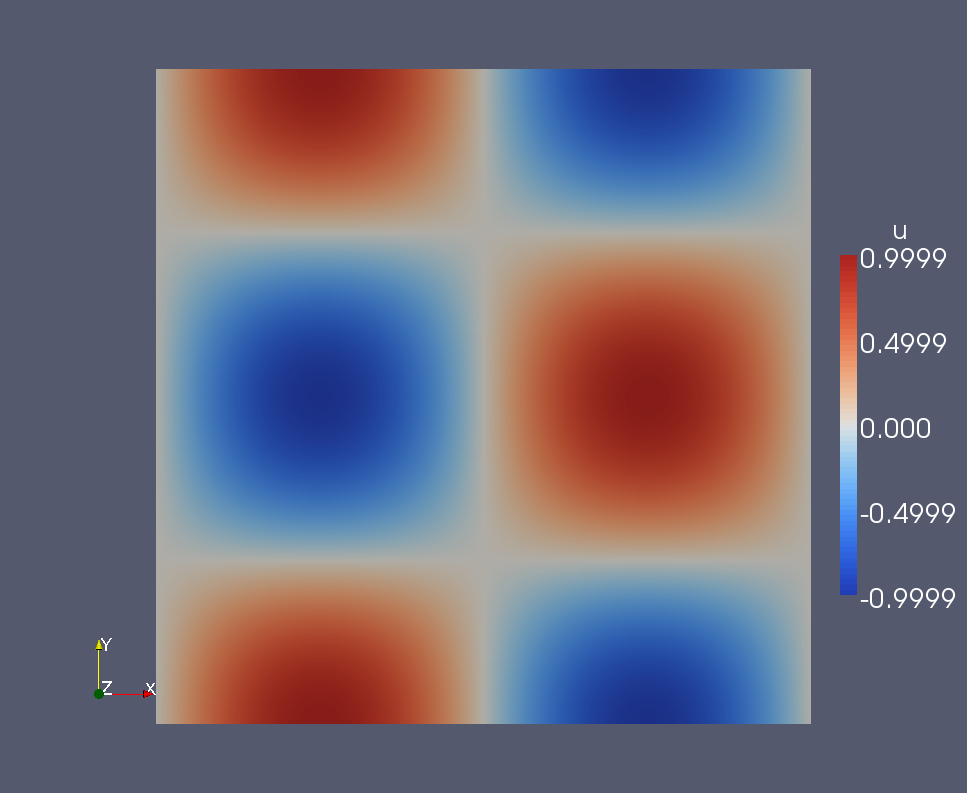
\includegraphics[width=.43\linewidth]{laplacian.png}}
  \subfigure[Elevation]{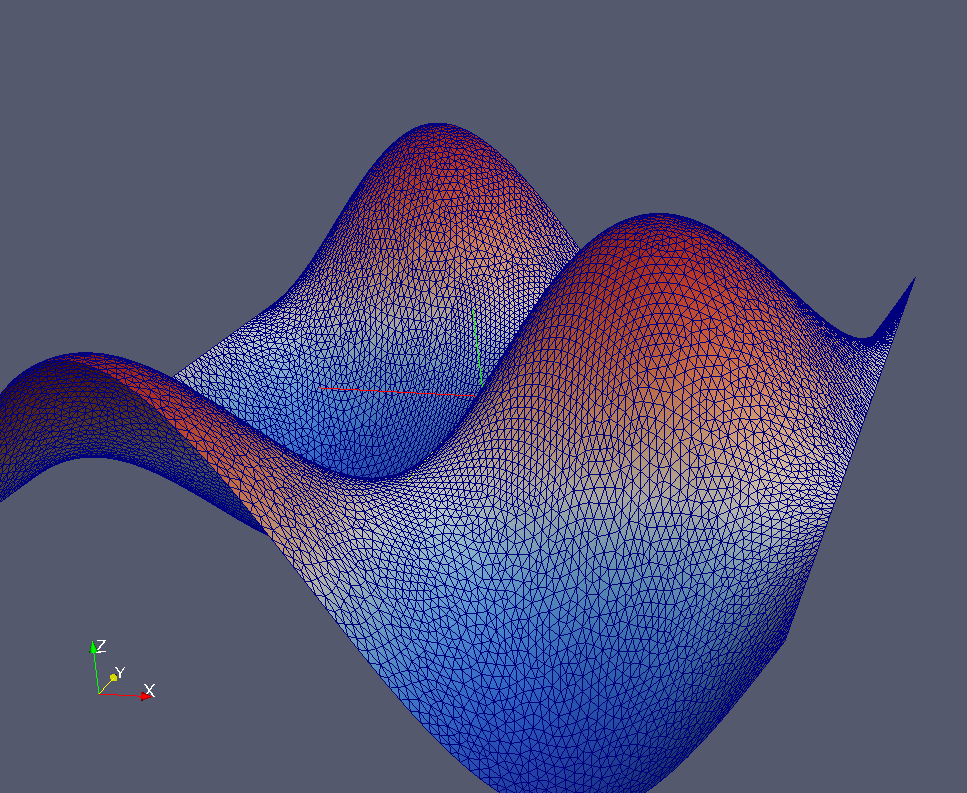
\includegraphics[width=.43\linewidth]{laplacian_warp.png}}
  \caption{Solution of problem~\ref{prob:3}}
  \label{fig:2}
\end{figure}

\subsection{Mixed formulation: the Stokes case}
\label{sec:mixed-form-stok}
\index{Stokes}
\subsubsection{Mathematical formulation}
\label{sec:math-form}

\index{Stokes!formulation!mathematical}
\marginpar{\lstinline!stokes.cpp!}  We are now interested in solving
the Stokes equations, we would like to solve for the following problem
in 2D
\begin{problem}
\label{prob:4}
 find $(\mathbf{u},p)$ such that
\begin{equation}
  \label{eq:22}
  - \mu \Delta \mathbf{u} +\nabla p = \mathbf{f}\quad \text{and}\quad \nabla \cdot \mathbf{u} = 0,\quad \text{in}\ \Omega = [-1;1]^2
\end{equation}
with
\begin{equation}
  \label{eq:24}
  \mathbf{f} = \mathbf{0}
\end{equation}
where $\mu$ being the viscosity. The following boundary conditions apply
\begin{equation}
  \label{eq:23}
  \mathbf{u}=\mathbf{1}_{|y=1}, \quad \mathbf{u}=\mathbf{0}_{|\partial \Omega \backslash \{(x,y) \in \Omega | y=1\}}
\end{equation}
\end{problem}

In problem (\ref{prob:2}), $p$ is known up to a constant $c$,
\emph{i.e.} if $p$ is a solution then $p+c$ is also solution. To
ensure uniqueness we impose the constraint that $p$ should have
zero-mean, \emph{i.e.}
\begin{equation}
  \label{eq:26}
  \int_\Omega p = 0
\end{equation}

The problem~\ref{prob:4} now reads
\begin{problem}
  \label{prob:5}
 find $(\mathbf{u},p,\lambda)$ such that
\begin{equation}
  \label{eq:34}
  - \mu \Delta \mathbf{u} +\nabla p = \mathbf{f}\quad, \quad \nabla \cdot \mathbf{u} + \lambda = 0, \quad \text{and}\quad \int_\Omega p = 0,\quad \text{in}\ \Omega = [-1;1]^2
\end{equation}
with
\begin{equation}
  \label{eq:35}
  \mathbf{f} = \mathbf{0}
\end{equation}
where $\mu$ being the viscosity. The following boundary conditions apply
\begin{equation}
  \label{eq:36}
  \mathbf{u}=\mathbf{1}_{|y=1}, \quad \mathbf{u}=\mathbf{0}_{|\partial \Omega \backslash \{(x,y) \in \Omega | y=1\}}
\end{equation}
\end{problem}

The functional framework is as follows, we look for $\mathbf{u}$ is
$H^1_0(\Omega)$ and $p$ in $L^2_0(\Omega)$. We shall not seek $p$ in
$L^2_0(\Omega)$ but rather in $L^2(\Omega)$ and use Lagrange
multipliers which live are the constants whose space we denote
$\mathbb{P}_0(\Omega)$, to enforce~(\ref{eq:26}).

Denote $\mathcal{X} = H^1_0(\Omega)\times
L^2(\Omega)\times\mathbb{P}_0(\Omega)$, the variational formulation
reads we look for $(\mathbf{u}, p, \lambda) \in \mathcal{X}$ for all
$(\mathbf{v},q,\nu) \in \mathcal{X}$
\begin{equation}
  \label{eq:25}
  \int_\Omega \mu \nabla \mathbf{u} : \nabla \mathbf{v} + \nabla \cdot \mathbf{v} p + \nabla \cdot \mathbf{u}\ q + q \lambda + p \nu  \ = \ \int_\Omega \mathbf{f} \cdot \mathbf{v}
\end{equation}

We build a triangulation $\Omega_h$ of $\Omega$, we choose compatible
(piecewise polynomial) discretisation spaces $X_h$ and $M_h$,
\emph{e.g.} the Taylor Hood element ($\mathbb{P}_N/\mathbb{P}_{N-1}$)
and we denote $\mathcal{X}_h=X_h\times M_h \times
\mathbb{P}_0(\Omega)$.  The discrete problem now reads, we look for
$(\mathbf{u}_h,p_h,\lambda_h) \in \mathcal{X}_h$ such that for all
$(\mathbf{v}_h,q_h,\nu_h) \in \mathcal{X}_h$
\begin{equation}
  \label{eq:27}
  \int_{\Omega_h} \mu \nabla \mathbf{u}_h \cdot \nabla \mathbf{v}_h + \nabla \cdot \mathbf{v}_h \ p_h + \nabla \cdot \mathbf{u}_h\ q_h + p_h \nu_h + q_h \lambda_h   = \ \int_{\Omega_h} \mathbf{f} \cdot \mathbf{v}_h
\end{equation}

The formulation~(\ref{eq:27}) leads to a linear system of the form
\begin{equation}
  \label{eq:28}
  \underbrace{\begin{pmatrix}
    A & B & 0\\
    B^T & 0 & C\\
    0 & C^T & 0
  \end{pmatrix}}_{\mathcal{A}}
\underbrace{
  \begin{pmatrix}
    \mathbf{u}_h\\
    p_h\\
    \lambda_h
  \end{pmatrix}}_{\mathcal{U}} =
\underbrace{\begin{pmatrix}
    F\\
    0\\
    0
  \end{pmatrix}}_{\mathcal{F}}
\end{equation}

where $A$ corresponds to the $(\mathbf{u},\mathbf{v})$ block, $B$ to
the $(\mathbf{u},q)$ block and $C$ to the $(p,\nu)$
block. $\mathcal{A}$ is a symetric positive definite matrix and thus
the system $\mathcal{A} \mathcal{U} = \mathcal{F}$ enjoys a unique
solution.

\subsubsection{Feel formulation}
\label{sec:feel-formulation}

\index{Stokes!formulation!feel}
Regarding the implementation of the Stokes problem~\ref{prob:4}, we
can start from the laplacian case, from
section~\ref{sec:defin-bilin-forms}. The implementation we choose to
display here defines and builds $\mathcal{X}_h$, $\mathcal{A}$,
$\mathcal{U}$ and $\mathcal{F}$.

We start by defining and building $\mathcal{X}_h$: first we define the
basis functions that will span each subspaces $X_h$, $M_h$ and
$\mathbb{P}_0(\Omega)$.

\lstinputlisting[linerange=marker1-endmarker1]{stokes.cpp}

note that on the \lstinline!typedef! we build a (MPL) vector of them. Now we are
ready to define the functionspace $\mathcal{X}_h$, much like in the
Laplacian case:

\lstinputlisting[linerange=marker2-endmarker2]{stokes.cpp}

Next we define a few types which are associated with $\mathcal{U}$,
$u$, $p$ and $\lambda$ respectively.

\lstinputlisting[linerange=marker3-endmarker3]{stokes.cpp}

Using these types we can instantiate elements of $\mathcal{X}_h$,
$X_h$, $M_h$ and $\mathbb{P}_0(\Omega_h)$ respectively:

\lstinputlisting[linerange=marker4-endmarker4]{stokes.cpp}

They will serve in the definition of the variational formulation. We
can now start assemble the various terms of the variational
formulation~(\ref{eq:27}). First we define some viscous stress tensor,
%$\tau(\mathbf{u}) = \frac{1}{2}(\nabla \mathbf{u} + \nabla \mathbf{u}^T)$,
$\tau(\mathbf{u}) = \nabla \mathbf{u}$,
associated with the trial and test functions
respectively

\lstinputlisting[linerange=marker5-endmarker5]{stokes.cpp}

Then we define the total stress tensor times the normal,
$\bar{\sigma}(\mathbf{u},p) \mathbf{n} = -p \mathbf{n} + 2 \mu \tau(\mathbf{u})
\mathbf{n}$ where $\mathbf{n}$ is the normal and $\bar{\sigma}(\mathbf{u},p) =
-p \mathbb{I} + 2 \mu \tau(\mathbf{u})$:

\lstinputlisting[linerange=marker6-endmarker6]{stokes.cpp}


We then form the matrix $\mathcal{A}$ starting with block $A$,  block $B$
block $C$ and finally the boundary conditions.


\lstinputlisting[linerange=marker7-endmarker7]{stokes.cpp}

The figure~\ref{fig:2} displays $p$ and $\mathbf{u}$ which are available in
\begin{unixcom}
  ls ~/feel/doc/tutorial/stokes/Simplex_2_1_2/P2/h_0.05
\end{unixcom}

\begin{figure}[htbp]
  \centering
  \subfigure[Colored with $p$, $h=0.05$]{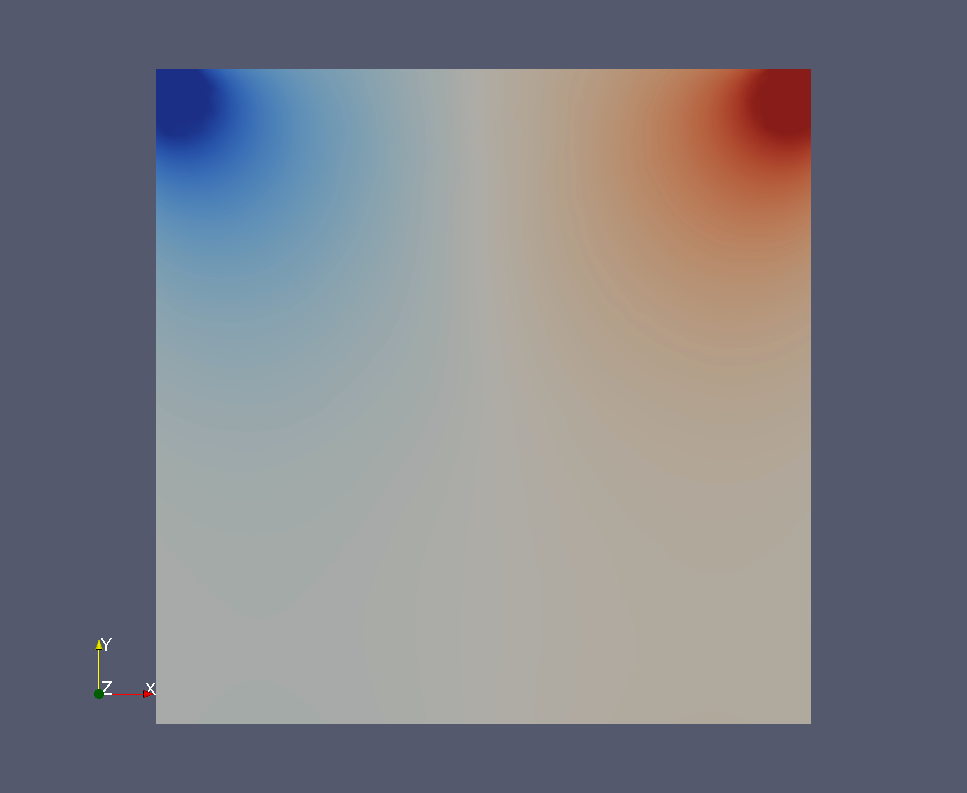
\includegraphics[width=.43\linewidth]{stokes-p.png}}
  \subfigure[Colored with $\|\mathbf{u}\|$ and the arrows associated to $\mathbf{u}$ colored with $p$]{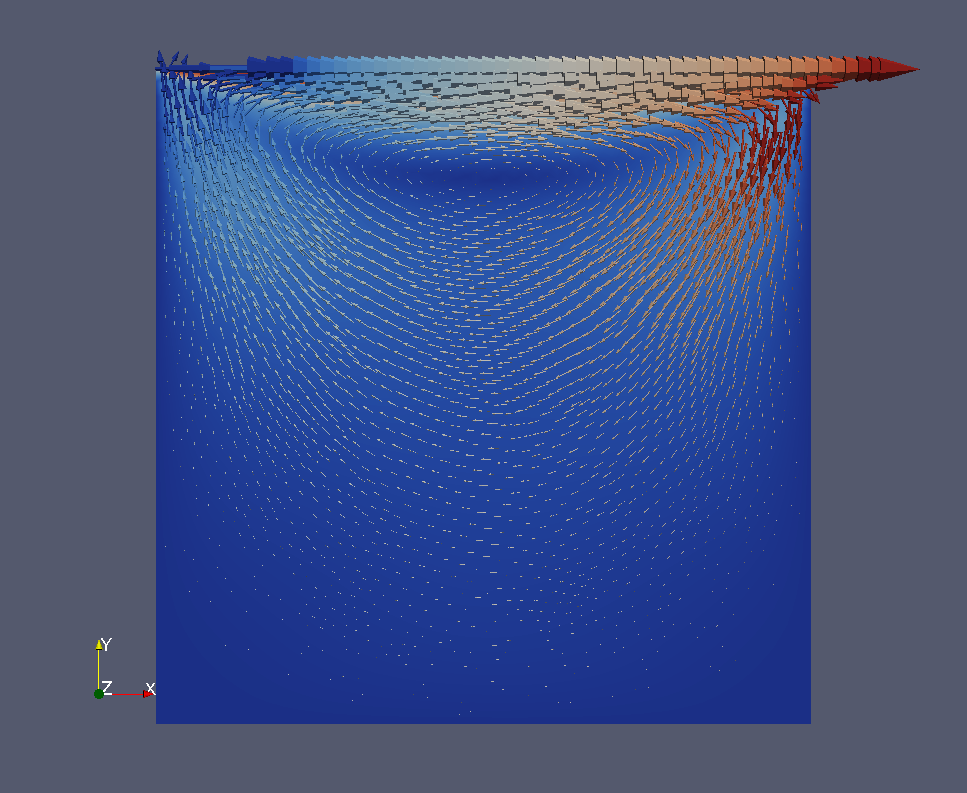
\includegraphics[width=.43\linewidth]{stokes-u.png}}
  \caption{Solution of problem~\ref{prob:4}}
  \label{fig:2}
\end{figure}

%%% Local Variables:
%%% coding: utf-8
%%% mode: latex
%%% TeX-PDF-mode: t
%%% TeX-parse-self: t
%%% x-symbol-8bits: nil
%%% TeX-auto-regexp-list: TeX-auto-full-regexp-list
%%% TeX-master: "../feel-manual"
%%% ispell-local-dictionary: "american"
%%% End:


\feelchapter{Feel++ Language Keywords}
            {Feel++ Language Keywords}
            {Christophe Prud'homme}
            {cha:appendix-feel}

One of Life assets is it finite element embedded language
(\feel). The language follows the C++ grammar, and provides keywords
as well as operations between objects which are, mathematically,
tensors of rank 0, 1 or 2.

Some notations
\begin{itemize}
\item $f: \mathbb{R}^n \mapsto \mathbb{R}^{m\times p}$  with $n=1,2,3$, $m=1,2,3$, $p=1,2,3$.
\item $\Omega^e$ current mesh element
\end{itemize}


\begin{longtable}[c]{rllll}
  Keyword & Math object & Description & Rank & $M \times N$\\\hline\hline

  \endhead
  %%
  %% Point
  %%
  \lstinline!P()! & $\overrightarrow{P}$ & current point coordinates $(P_x, P_y, P_z)^T$ & 1 & $d \times 1$ \\

  \lstinline!Px()! & $P_x$ & $x$ coordinate of $\overrightarrow{P}$ & 0 & $1 \times 1$\\

  \lstinline!Py()! & $P_y$ & $y$ coordinate of $\overrightarrow{P}$ & 0 & $1 \times 1$\\
  & &  (value is 0 in 1D) & &\\

  \lstinline!Pz()! & $P_z$ & $z$ coordinate of $\overrightarrow{P}$& 0 & $1 \times 1$\\
  & &  (value is 0 in 1D and 2D)  & &\\\hline\\

  %%
  %% Barycenter
  %%
  \lstinline!C()! & $\overrightarrow{C}$ & element barycenter point coordinates  & 1 & $d \times 1$ \\
  &&$(C_x, C_y, C_z)^T$&&\\

  \lstinline!Cx()! & $C_x$ & $x$ coordinate of $\overrightarrow{C}$ & 0 & $1 \times 1$\\

  \lstinline!Cy()! & $C_y$ & $y$ coordinate of $\overrightarrow{C}$ & 0 & $1 \times 1$\\
  & &  (value is 0 in 1D) & &\\

  \lstinline!Cz()! & $C_z$ & $z$ coordinate of $\overrightarrow{C}$& 0 & $1 \times 1$\\
  & &  (value is 0 in 1D and 2D)  & &\\\hline\\

  %%
  %% normal
  %%

  \lstinline!N()! & $\overrightarrow{N}$ & normal at current point $(N_x,N_y,N_z)^T$ & 1 & $d \times 1$\\

  \lstinline!Nx()! & $N_x$ & $x$ coordinate of $\overrightarrow{N}$ at current point & 0 & $1 \times 1$\\

  \lstinline!Ny()! & $N_y$ & $y$ coordinate of $\overrightarrow{N}$ at current point & 0 & $1 \times 1$\\
  & &  (value is 0 in 1D) & &\\

  \lstinline!Nz()! & $N_z$ & $z$ coordinate of $\overrightarrow{N}$ at current point& 0 & $1 \times 1$\\
  & &  (value is 0 in 1D and 2D)  & &\\\hline\\

  %%
  %% Element id
  %%
  \lstinline!eid()! & $e$ & index of  $\Omega^e$ & 0 & $1 \times 1$\\
  \lstinline!emarker()! & $m(e)$ & marker of  $\Omega^e$ & 0 & $1 \times 1$\\
  \lstinline!h()! & $h^e$ & size of   $\Omega^e$ & 0 & $1 \times 1$\\
  \lstinline!hFace()! & $h^e_{\Gamma}$ & size of face $\Gamma$ of $\Omega^e$ & 0 & $1 \times 1$\\\hline\\

  %%
  %% Mat/vec
  %%
  \lstinline!mat<M,N>(m_11,! &
  $\begin{pmatrix}
    m_{11} & m_{12} & ...\\
    m_{21} & m_{22} & ...\\
    \vdots & &
  \end{pmatrix}$
  & $M\times N$ matrix    & 2 & $M \times N$\\
  \lstinline!m_12,...)!& & entries being expressions   & &\\

  \lstinline!vec<M>(v_1,! &$(v_1, v_2,...)^T$
  & column vector with $M$ rows    & 1 & $M \times 1$\\
  \lstinline!v_2,...)!& & entries being expressions   & &\\

  \lstinline!trace(expr)! &$\mathrm{tr}(f(\overrightarrow{x}))$  & trace of $f(\overrightarrow{x})$   & 0 & $1 \times 1$\\\hline\\


  %%
  %% std math functions
  %%

  \lstinline!abs(expr)! & $|f(\overrightarrow{x})|$ & element wise absolute value of $f$ & $\mathrm{rank}(f(\overrightarrow{x}))$ & $m \times p$\\
  \lstinline!cos(expr)! & $\cos(f(\overrightarrow{x}))$ & element wise cosinus value of $f$ & $\mathrm{rank}(f(\overrightarrow{x}))$ & $m \times p$\\
  \lstinline!sin(expr)! & $\sin(f(\overrightarrow{x}))$ & element wise sinus value of $f$ & $\mathrm{rank}(f(\overrightarrow{x}))$ & $m \times p$\\
  \lstinline!tan(expr)! & $\tan(f(\overrightarrow{x}))$ & element wise tangent value of $f$ & $\mathrm{rank}(f(\overrightarrow{x}))$ & $m \times p$\\
  \lstinline!acos(expr)! & $\acos(f(\overrightarrow{x}))$ & element wise acos value of $f$ & $\mathrm{rank}(f(\overrightarrow{x}))$ & $m \times p$\\
  \lstinline!asin(expr)! & $\asin(f(\overrightarrow{x}))$ & element wise asin value of $f$ & $\mathrm{rank}(f(\overrightarrow{x}))$ & $m \times p$\\
  \lstinline!atan(expr)! & $\atan(f(\overrightarrow{x}))$ & element wise atan value of $f$ & $\mathrm{rank}(f(\overrightarrow{x}))$ & $m \times p$\\
  \lstinline!cosh(expr)! & $\cosh(f(\overrightarrow{x}))$ & element wise cosh value of $f$ & $\mathrm{rank}(f(\overrightarrow{x}))$ & $m \times p$\\
  \lstinline!sinh(expr)! & $\sinh(f(\overrightarrow{x}))$ & element wise sinh value of $f$ & $\mathrm{rank}(f(\overrightarrow{x}))$ & $m \times p$\\
  \lstinline!tanh(expr)! & $\tanh(f(\overrightarrow{x}))$ & element wise tanh value of $f$ & $\mathrm{rank}(f(\overrightarrow{x}))$ & $m \times p$\\
  \lstinline!exp(expr)! & $\exp(f(\overrightarrow{x}))$ & element wise exp value of $f$ & $\mathrm{rank}(f(\overrightarrow{x}))$ & $m \times p$\\
  \lstinline!log(expr)! & $\log(f(\overrightarrow{x}))$ & element wise log value of $f$ & $\mathrm{rank}(f(\overrightarrow{x}))$ & $m \times p$\\
  \lstinline!sqrt(expr)! & $\sqrt{f(\overrightarrow{x})}$ & element wise sqrt value of $f$ & $\mathrm{rank}(f(\overrightarrow{x}))$ & $m \times p$\\
  \lstinline!sign(expr)! & $
  \begin{cases}
    1 & \text{if}\ f(\overrightarrow{x}) \geq 0\\
    -1 & \text{if}\ f(\overrightarrow{x}) < 0
  \end{cases}$ & element wise sign of $f$ & $\mathrm{rank}(f(\overrightarrow{x}))$ & $m \times p$\\
  \lstinline!chi(expr)! & $\chi(f(\overrightarrow{x}))=$ & element wise boolean test of $f$ & $\mathrm{rank}(f(\overrightarrow{x}))$ & $m \times p$\\
  & $\begin{cases}
    0 & \text{if}\ f(\overrightarrow{x}) = 0\\
    1 & \text{if}\ f(\overrightarrow{x}) \neq 0\\
  \end{cases}$ &&&\\\hline\\

  %%
  %% operation
  %%
  \lstinline!id(f)! & $f$ & test function & $\mathrm{rank}(f(\overrightarrow{x}))$ & $m \times p$\\
  \lstinline!idt(f)! & $f$ & trial function & $\mathrm{rank}(f(\overrightarrow{x}))$ & $m \times p$\\
  \lstinline!idv(f)! & $f$ & evaluation function   & $\mathrm{rank}(f(\overrightarrow{x}))$ & $m \times p$\\
  \lstinline!grad(f)! & $\nabla f$ & gradient of test function & $\mathrm{rank}( f(\overrightarrow{x}))+1$ & $p=1,\ m \times n$\footnote{Gradient of matrix value functions is not implemented, hence $p=1$ }\\
  \lstinline!gradt(f)! & $\nabla f$ & gradient of trial function & $\mathrm{rank}(f(\overrightarrow{x}))+1$ & $p=1,\ m \times n$\\
  \lstinline!gradv(f)! & $\nabla f$ & evaluation function gradient    & $\mathrm{rank}(f(\overrightarrow{x}))+1$ & $p=1,\ m \times n$\\

  \lstinline!div(f)! & $\nabla \cdot \overrightarrow{f}$ & divergence of test function & $\mathrm{rank}( f(\overrightarrow{x}))-1$ & $1\times 1$\footnote{Divergence  of matrix value functions is not implemented, hence $p=1$ }\\
  \lstinline!divt(f)! & $\nabla \cdot \overrightarrow{f}$ & divergence of trial function & $\mathrm{rank}( f(\overrightarrow{x}))-1$ & $1\times 1$\\
  \lstinline!divv(f)! & $\nabla \cdot \overrightarrow{f}$ & evaluation of  function divergence  & $\mathrm{rank}( f(\overrightarrow{x}))-1$ & $1\times 1$\\

  \lstinline!curl(f)! & $\nabla \times \overrightarrow{f}$ & curl of test function & 1 & $n=m, n\times 1$\\
  \lstinline!curlt(f)! & $\nabla \times \overrightarrow{f}$ & curl of trial function & 1 & $m=n, n\times 1$\\
  \lstinline!curlv(f)! & $\nabla \times \overrightarrow{f}$ & evaluation of  function curl  & 1 & $m=n, n\times 1$\\

  \lstinline!hess(f)! & $\nabla^2 f$ & hessian of test function & 2 & $m=p=1, n\times n$\\\hline\\

  %%
  %% Two valued operators
  %%
  \lstinline!jump(f)! & $[f]=f_0\overrightarrow{N_0}+f_1\overrightarrow{N_1}$ & jump of test function & 1   & $m=1, n\times 1$\\
  \lstinline!jump(f)! & $[\overrightarrow{f}]=\overrightarrow{f_0}\cdot\overrightarrow{N_0}+\overrightarrow{f_1}\cdot\overrightarrow{N_1}$ & jump of test function & 0   & $m=2, 1\times 1$\\
  \lstinline!jumpt(f)! & $[f]=f_0\overrightarrow{N_0}+f_1\overrightarrow{N_1}$ & jump of trial function & 1   & $m=1, n\times 1$\\
  \lstinline!jumpt(f)! & $[\overrightarrow{f}]=\overrightarrow{f_0}\cdot\overrightarrow{N_0}+\overrightarrow{f_1}\cdot\overrightarrow{N_1}$ & jump of trial function & 0   & $m=2, 1\times 1$\\
  \lstinline!jumpv(f)! & $[f]=f_0\overrightarrow{N_0}+f_1\overrightarrow{N_1}$ & jump of  function evaluation & 1   & $m=1, n\times 1$\\
  \lstinline!jumpv(f)! & $[\overrightarrow{f}]=\overrightarrow{f_0}\cdot\overrightarrow{N_0}+\overrightarrow{f_1}\cdot\overrightarrow{N_1}$ & jump of  function evaluation & 0   & $m=2, 1\times 1$\\
  \lstinline!average(f)! & ${f}=\frac{1}{2}(f_0+f_1)$ & average of test function & $\mathrm{rank}( f(\overrightarrow{x}))$   & $m=n, n\times n$\\
  \lstinline!averaget(f)! & ${f}=\frac{1}{2}(f_0+f_1)$ & average of trial function & $\mathrm{rank}( f(\overrightarrow{x}))$   & $m=n, n\times n$\\
  \lstinline!averagev(f)! & ${f}=\frac{1}{2}(f_0+f_1)$ & average of  function evaluation & $\mathrm{rank}( f(\overrightarrow{x}))$   & $m=n, n\times n$\\

  \lstinline!leftface(f)! & $f_0$ & left  test function & $\mathrm{rank}( f(\overrightarrow{x}))$   & $m=n, n\times n$\\
  \lstinline!leftfacet(f)! & $f_0$ & left  trial function & $\mathrm{rank}( f(\overrightarrow{x}))$   & $m=n, n\times n$\\
  \lstinline!leftfacev(f)! & $f_0$ & left   function evaluation & $\mathrm{rank}( f(\overrightarrow{x}))$   & $m=n, n\times n$\\
  \lstinline!rightface(f)! & $f_1$ & right  test function & $\mathrm{rank}( f(\overrightarrow{x}))$   & $m=n, n\times n$\\

  \lstinline!rightfacet(f)! & $f_1$ & right  trial function & $\mathrm{rank}( f(\overrightarrow{x}))$   & $m=n, n\times n$\\
  \lstinline!rightfacev(f)! & $f_1$ & right   function evaluation & $\mathrm{rank}( f(\overrightarrow{x}))$   & $m=n, n\times n$\\

  \lstinline!maxface(f)! & $\max(f_0,f_1)$ & maximum of right and left & $\mathrm{rank}( f(\overrightarrow{x}))$   & $m\times p$\\
  && test   function&&\\
  \lstinline!maxfacet(f)! & $\max(f_0,f_1)$ & maximum of right and left & $\mathrm{rank}( f(\overrightarrow{x}))$   & $m\times p$\\
  && trial   function&&\\
  \lstinline!maxfacev(f)! & $\max(f_0,f_1)$ & maximum of right and left & $\mathrm{rank}( f(\overrightarrow{x}))$   & $m\times p$\\
  && function evaluation&&\\
  \lstinline!minface(f)! & $\min(f_0,f_1)$ & minimum of right and left & $\mathrm{rank}( f(\overrightarrow{x}))$   & $m\times p$\\
  && test   function&&\\
  \lstinline!minfacet(f)! & $\min(f_0,f_1)$ & minimum of right and left & $\mathrm{rank}( f(\overrightarrow{x}))$   & $m\times p$\\
  && trial   function&&\\
  \lstinline!minfacev(f)! & $\min(f_0,f_1)$ & minimum of right and left & $\mathrm{rank}( f(\overrightarrow{x}))$   & $m\times p$\\
  && function evaluation&&\\
  \hline\\
  %%
  %% Operations
  %%
  \lstinline!-! & $-g$ & element wise unary minus  & & \\
  \lstinline!-! & $!g$ & element wise logical not  & & \\\hline\\

  \lstinline!+! & $f+g$ & tensor sum  & & \\
  \lstinline!-! & $f-g$ & tensor substraction  & & \\
  \lstinline!*! & $f*g$ & tensor product  & & \\
  \lstinline!/! & $f/g$ & tensor division ($g$ scalar field)  & & \\\hline\\

  \lstinline!<! & $f < g$ & element wise less  & & \\
  \lstinline!<=! & $f \leq g$ & element wise less or equal  & & \\
  \lstinline!>! & $f > g$ & element wise greater  & & \\
  \lstinline!>=! & $f \geq g$ & element wise greater or equal  & & \\
  \lstinline!==! & $f = g$ & element wise  equal  & & \\
  \lstinline+!=+ & $f \neq g$ & element wise not equal  & & \\
  \lstinline!&&! & $f\ \text{and}\ g$ & element wise logical and  & & \\
  \lstinline!||! & $f\ \text{or}\ g$ & element wise logical or  & & \\\hline\\


\end{longtable}
%%% Local Variables:
%%% coding: utf-8
%%% mode: latex
%%% TeX-PDF-mode: t
%%% TeX-parse-self: t
%%% x-symbol-8bits: nil
%%% TeX-auto-regexp-list: TeX-auto-full-regexp-list
%%% TeX-master: "feel-manual"
%%% ispell-local-dictionary: "american"
%%% End:



\part{Learning by Examples}
\label{part:learning-examples}

\feelchapter{Non-Linear examples}
            {Non-Linear examples}
            {Christophe Prud'homme}
            {cha:non-linear-ex}

\section{Solving nonlinear equations}
\label{sec:nonlinear-equations}

\feel allows to solve nonlinear equations thanks to its interface to
the interface to the PETSc nonlinear solver library. It requires the
implementation of two extra functions in your application that will
update the jacobian matrix associated to the tangent problem and the
residual.

Consider that you have an application class \lstinline!MyApp! with a
backend as data member
\begin{lstlisting}{gobble=2}
#include <feel/feelcore/feel.hpp>
#include <feel/feelcore/application.hpp>
#include <feel/feelalg/backend.hpp>
namespace Feel {

class MyApp : public Application
{
  public:

  typedef Backend<double> backend_type;
  typedef boost::shared_ptr<backend_type> backend_ptrtype;

  MyApp( int argc, char** argv,
  AboutData const& ad, po::options_description const& od )
  :
  // init the parent class
  Application( argc, argv, ad, od ),
  // init the backend
  M_backend( backend_type::build( soption("backend") ) ),
  {
    // define the callback functions (works only for the PETSc backend)
    M_backend->nlSolver()->residual =
      boost::bind( &self_type::updateResidual, boost::ref( *this ), _1, _2 );
    M_backend->nlSolver()->jacobian =
      boost::bind( &self_type::updateJacobian, boost::ref( *this ), _1, _2 );

  }
  void updateResidual( const vector_ptrtype& X, vector_ptrtype& R )
  {
    // update the matrix J (Jacobian matrix) associated
    // with the tangent problem
  }
  void updateJacobian( const vector_ptrtype& X, sparse_matrix_ptrtype& J)
  {
    // update the vector R associated with the residual
  }
  void run()
  {

    //define space
    Xh...
    element_type u(Xh);
    // initial guess is 0
    u = project( M_Xh, elements(mesh), constant(0.) );
    vector_ptrtype U( M_backend->newVector( u.functionSpace() ) );
    *U = u;

    // define R and J
    vector_ptrtype R( M_backend->newVector( u.functionSpace() ) );
    sparse_matrix_ptrtype J;

    // update R
    updateJacobian( U, R );
    // update J
    updateResidual( U, J );

    // solve using non linear methods (newton)
    // tolerance : 1e-10
    // max number of iterations : 10
    M_backend->nlSolve( J, U, R, 1e-10, 10 );

    // the soluution was stored in U
    u = *U;
  }
  private:

  backend_ptrtype M_backend;
};
} // namespace Feel
\end{lstlisting}

The function \lstinline!updateJacobian! and \lstinline!updateResidual!
implement the assmebly of the matrix $J$ (jacobian matrix) and the
vector $R$ (residual vector) respectively.

\subsection{A first nonlinear problem}
\label{sec:bratu}

As a simple example, let $\Omega$ be a subset of $\mathbb{R}^d, d=1,2,3$,
(\emph{i.e.} $\Omega=[-1,1]^d$) with boundary $\partial
\Omega$. Consider now the following equation and boundary condition
\begin{equation}
  \label{eq:29}
  -\Delta u + u^\lambda = f,\quad u = 0 \text{ on } \partial \Omega.
\end{equation}
where $\lambda \in \mathbb{R_+}$ is a given parameter and $f=1$.


\begin{nota}
  To be described in this section. For now see
  \texttt{doc/manual/nonlinearpow.cpp} for an implementation of this
  problem.
\end{nota}

\subsection{Simplified combustion problem: Bratu}
\label{sec:bratu}

As a simple example, let $\Omega$ be a subset of $\mathbb{R}^d, d=1,2,3$,
(\emph{i.e.} $\Omega=[-1,1]^d$) with boundary $\partial
\Omega$. Consider now the following equation and boundary condition
\begin{equation}
  \label{eq:29}
  -\Delta u + \lambda e^u = f,\quad u = 0 \text{ on } \partial \Omega
\end{equation}
where $\lambda$ is a given parameter. Ceci est généralement appellé le
problème de Bratu et apparaît lors de la simplification de modèles de
processus de diffusion non-linéaires par exemple dans le domaine de la
combustion.

\begin{nota}
  To be described in this section. For now see
  \texttt{doc/manual/bratu.cpp} for an implementation of this
  problem.
\end{nota}

%%% Local Variables:
%%% coding: utf-8
%%% mode: latex
%%% TeX-PDF-mode: t
%%% TeX-parse-self: t
%%% x-symbol-8bits: nil
%%% TeX-auto-regexp-list: TeX-auto-full-regexp-list
%%% TeX-master: "../feel-manual"
%%% ispell-local-dictionary: "american"
%%% End:


\feelchapter{Heat sink}
            {Heat sink}
            {Baptiste Morin, Christophe Prud'homme}
            {cha:heatsink}

This problem considers the performance of a heat sink designed for the thermal management of high-density electronic components. The heat sink is comprised of a base/spreader which in turn supports a number of plate fins exposed to flowing air. We model the flowing air through a simple convection heat transfer coefficient. From the engineering point of view, this problem illustrates the application of conduction analysis to an important class of cooling problems: electronic components and systems. \\ \\
Our interest is in the conduction temperature distribution at the base of the spreader. The target is to study how the heat transfer occures with different parameters on our heat sink. The heat generated by high-density electronic components is such that it's very expensive to cool large structures (data center). The cooling optimization is consequent in the run for decreasing operating costs.

\noindent A classical thermal CPU cooler looks like this 

\begin{figure}[!h]
\centering
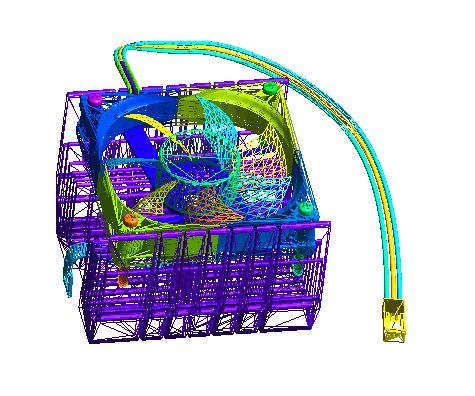
\includegraphics[width=.45\linewidth]{heatsink/complete_cooler.png}
\caption{Mesh of a classical CPU cooler}
\end{figure}

\noindent We are here going to describe how it is theorically working and how it is impleted with \feel. 

\section{Problem description}
\subsection{Domain}

We consider here a classical "radiator" which is a CPU heat sink. Those types of coolers are composed with a certain number of plate fins exposed to flowing air or exposed to a ventilator. Regarding the periodicity and geometry of our concern, we can make our study on a characteristic element of the problem : a half cell of the heat sink single thermal fin with its spreader at the basis. Let's take a look at the geometry of our problem :

\begin{figure}[!h]
\centering
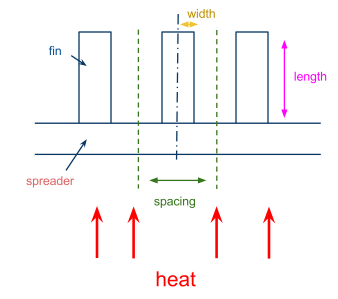
\includegraphics[width=.45\linewidth]{heatsink/sink_geom.png}
\caption{Geometry of heat sink}
\end{figure}

Our study is avaible in 2 or 3 dimensions, depending on the application's parameters. You'll see later how to work with it. Let's see on which meshes we are working on :
\begin{figure}[!h]
\begin{minipage}[b]{.50\linewidth}
\centering
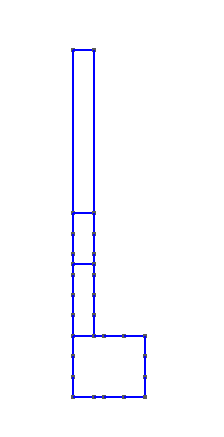
\includegraphics[width=.45\linewidth]{heatsink/mesh_2d.png}
\caption{2D mesh}
\end{minipage}
\begin{minipage}[b]{.50\linewidth}
\centering

\includegraphics[width=.65\linewidth]{heatsink/mesh_3d.png}
\caption{3D mesh}
\end{minipage}
\end{figure}

\subsection{Parameters}
The implementation of thoses parameters is described in the section ~\ref{heat:param}.

\subsubsection{Material}

Here the material parameter can be described with furthers parameters. We have, with $i=1$ for the fin and $i=2$ for the base :
\begin{itemize}
\item the thermal conductivity $\kappa_i$

\item the material's density $\rho_i$

\item the heat capacity of the material $C_i$

\end{itemize}
The term $\rho_i C_i$ corresponds to the heat volumetric capacity. In that way, we make possible the construction of a heat sink with $2$ different materials. Here is a list of the well-known ones, $\rho$ and $C$ are gave at $298 K$ :

\begin{center}
\begin{tabular}{|c|c|c|c|}
  \hline
  \textbf{Material} & \textbf{Thermal conductivity} ($\kappa$ in $W.m^{-1}.K^{-1}$) & \textbf{Density }($\rho$ in $kg.m^{-3}$) & \textbf{Heat Capacity} ($C$ in $J.kg^{-1}.K^{-1}$) \\
  \hline
  Aluminium & 180 (alloys) or 290 (pure) & 2700 & 897 \\
  \hline
  Copper & 386 & 8940 & 385 \\
  \hline
  Gold & 314 & 19320 & 129 \\
  \hline
  Silver & 406 & 10500 & 233 \\
  \hline
\end{tabular}
\end{center}

\subsubsection{Depth}
This parameter is only to take into account for the 3D simulation. It represents the depth of the caracteristical heat sink and is called \lstinline!depth! in the application.

\subsubsection{Width}
Typically, this parameter is linked with constructor's standards. This parameter is called \lstinline!width! in the application's implementation.

\subsubsection{Summary table}
The table following table displays the various fixed and variables parameters of this application.
\clearpage

\begin{table}[htbp]
  \centering
  \begin{tabular}{@{}llrrr@{}} \toprule
Name & Description & Nominal Value & Range & Units \\ \midrule
\multicolumn{2}{c}{BDF parameters} \\ \cmidrule(r){1-2}
$time-initial$ & begining & $0$ & &  \\
$time-final$ & end & $50$ & $]0, 1500]$ &  \\
$time-step$ & time step & $0.1$ & $]0,1[$ &  \\
$steady$ & steady state & $0$ & $\{0,1\}$ &  \\
$order$ & order & $2$ & $[0, 4]$ & \\\\

\multicolumn{2}{c}{Physical parameters} \\ \cmidrule(r){1-2}
$L$ & fin's length & $2\cdot 10^{-2}$ & $[0.02, 0.05]$ & $m$ \\
$width$ & fin's width & $5\cdot 10^{-4}$ & $[10^{-5}, 10^{-4}]$ & $m$ \\
$deep$ & heat sink depth & $0$ & $[0, 7\cdot 10^{-2}]$ & $m$ \\\\

\multicolumn{2}{c}{Mesh parameter} \\ \cmidrule(r){1-2}
$hsize$ & mesh's size & $10^{-4}$ & $[10^{-5},10^{-3} ]$ & \\\\

\multicolumn{2}{c}{Fin Parameters} \\ \cmidrule(r){1-2}
$\kappa_f$ & thermal conductivity & $386$ & $[100,500] $ & $W \cdot m^{-1} \cdot K^{-1}$\\
$\rho_f$ & material density & $8940$ & $[10^3,12\cdot 10^3 ]$ & $kg\cdot m^{-3}$\\
$C_f$ & heat capacity & $385$ & $[10^2,10^3]$ & $J\cdot kg^{-1} \cdot K^{-1}$\\\\

\multicolumn{2}{c}{Base/spreader Parameters} \\ \cmidrule(r){1-2}
$\kappa_s$ & thermal conductivity & $386$ & $[100,500] $ & $W \cdot m^{-1} \cdot K^{-1}$\\
$\rho_s$ & material density & $8940$ & $[10^3,12\cdot 10^3 ]$ & $kg\cdot m^{-3}$\\
$C_s$ & heat capacity & $385$ & $[10^2,10^3]$ & $J\cdot kg^{-1} \cdot K^{-1}$\\\\

\multicolumn{2}{c}{Heat Parameters} \\ \cmidrule(r){1-2}
$T_{amb}$ & Inflow temperature & $300$ & [300,310] & $K$ \\
$heat\_flux$ & Heat flux $Q$ & $10^6$ & $[0 ,10^{6}]$ & $W \cdot m^{-3}$\\
$therm\_coeff$ & Thermal coefficient $h$ & $10^3$ & $[0,10^3]$ & $W\cdot m^{-2} \cdot K^{-1}$ \\
\end{tabular}

  \caption{Table of fixed and variable parameters}
  \label{tab:param}
\end{table}


\section{Theory}
\label{therm:equations}

\subsection{Figure}
The global domain is $\varOmega = \varOmega_1 \cup \varOmega_2 $ where $\varOmega_1$ is the fin's domain and $\varOmega_2$ the spreader's domain. We note $\partial\varOmega$ the border of the domain $\varOmega$. The physical lines we are using will be noted as $\Gamma_i$ such as described above. The following figure describes the parameters and the geometry we are using in the equations to solve our 3D issue :
The following figures describe the parameters and the geometry we are using in the equations to solve our 2D or 3D issue :
\begin{figure}[!h]
\centering
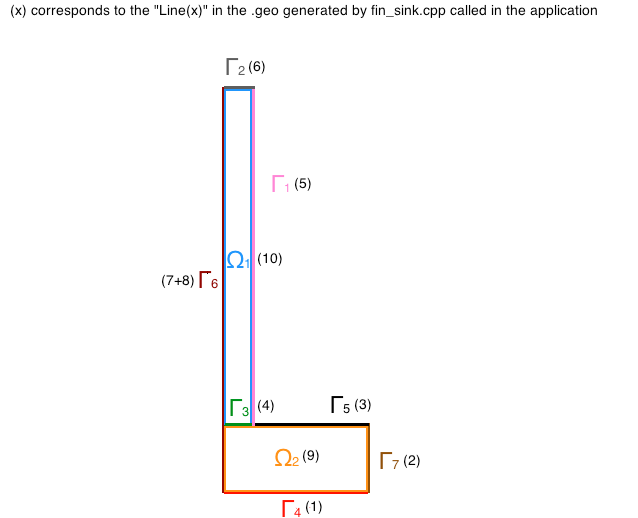
\includegraphics[width=.50\linewidth]{heatsink/figure_2d.png}
\caption{2D geometry details}
\end{figure}

\begin{figure}[!h]
\centering
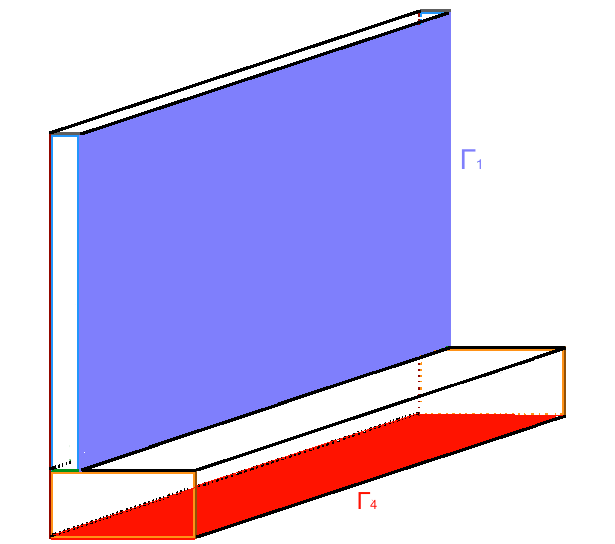
\includegraphics[width=.50\linewidth]{heatsink/figure_3d.png}
\caption{3D geometry details}
\end{figure}
\clearpage

\subsection{Equations}

Our concern satisfies the heat equation which reads 
\begin{equation}
\label{heat:eq}
   \begin{split}
      \displaystyle{\sum_{i=1}^{2} \kappa_i \Delta T - \rho_i C_i \frac{ \partial T}{\partial t}}  & = 0
  \end{split}
\end{equation}
\begin{equation}
\label{hom_neu1}
   \begin{split}
      \displaystyle{ \kappa_1 \frac{\partial T}{\partial n}} & =  0 \quad on \quad \Gamma_2 \quad and \quad \Gamma_6 \\ \\ 
  \end{split}
\end{equation}
\begin{equation}
\label{hom_neu2}
   \begin{split}
      \displaystyle{ \kappa_2 \frac{\partial T}{\partial n}} & =  0 \quad on \quad \Gamma_5 , \Gamma_7 \quad and \quad \Gamma_8 \\ \\ 
  \end{split}
\end{equation}
\begin{equation}
\label{classic_neu}
   \begin{split}
      \displaystyle{ \kappa_1 \frac{\partial T}{\partial n}} & = - h( T - T_{amb}) \quad on \quad \Gamma_1 \\ \\
  \end{split}
\end{equation}
\begin{equation}
\label{nonhom_neu}
   \begin{split}
      \displaystyle{ \kappa_2 \frac{\partial T}{\partial n}} & =  Q(1-e^{-t}) \quad on \quad \Gamma_4 \\ \\
  \end{split}
\end{equation}
\begin{equation}
\label{temp_conti}
   \begin{split}
      T_{| \varOmega_1} & = T_{| \varOmega_2} \quad on \quad \Gamma_3 \\ \\
  \end{split}
\end{equation}
\begin{equation}
\label{flux_conti}
   \begin{split}
      \displaystyle{ \kappa_1 \nabla T \cdot n} & = \displaystyle{ \kappa_2 \nabla T \cdot n \quad on \quad \Gamma_3} \\ \\
  \end{split}
\end{equation}

\noindent with $i=1$ for the fin and $i=2$ for the base and where $\kappa_i$ is the thermal conductivity, $\rho_i$ is the material's density ($kg.m^{-3}$ in the SI unit), $C_i$ the heat capacity and $T$ the temperature at a precise point (in 2D or 3D). To see how it has been coded, you can read \ref{heat:eq_impl}.


\subsection{Boundary conditions}
\label{heat:bc}
The problem requieres that the temperature and heat flux are continute on $\Gamma_3$. Considering the problem's geometry, we also impose zero heat flux on the vertical surfaces of the spreader. Let's detail the conditions we have imposed :
\begin{itemize}
\item Homogeneous Neumann condition (\ref{hom_neu1}) and (\ref{hom_neu2}) : it represents the fact that the heat flux is only vertical (for $\Gamma_6$ and $\Gamma_7$) or the fact that the heat flux is only provided by $\Gamma_4$ (for $\Gamma_2$ and $\Gamma_5$).

\item Homogeneous Neumann condition (\ref{classic_neu}) : it imposes that the heat flux is brought by this surface (it mathematically represents that the heat sink is placed on the heat source).

\item Non-homogeneous Neumann condition (\ref{nonhom_neu}) :  this boundary condition represents the transient state for the heat transfer calculation.

\item Temperature continuity (\ref{temp_conti}) : it imposes that the temperature is continute at the interface between the two materials (if there are two materials, we can also have the same one for the two pieces).

\item Heat flux continuity (\ref{flux_conti}) : it represents that the heat flux is continute at the interface between the two materials. Literally, it means that the two flows offset each other.

\end{itemize}

\noindent Theses conditions have been coded as explained in the section \ref{heat:eq_impl}.

\subsection{Finite Element Method}
Let's apply the method to our concern, we introduce the test function $v$ and we integrate the main equation, which reads now as :
\begin{equation}
   \begin{split}
      \displaystyle{\sum_{i=1}^{2} \rho_i C_i \int_{\varOmega_i} v\frac{ \partial T}{\partial t} - \kappa_i \int_{\varOmega_i} v\Delta T }  & = 0  
  \end{split}
\end{equation}
We integrate by parts, which leads to :
\begin{equation}
   \begin{split}
      \displaystyle{\sum_{i=1}^{2} \rho_i C_i \int_{\varOmega_i} v\frac{ \partial T}{\partial t} +  \kappa_i \int_{\varOmega_i} {\nabla v \cdot \nabla T} - \kappa_i \int_{\partial \varOmega_i} {(\nabla T \cdot n) v} }  & = 0
  \end{split}
\end{equation}
then, by decomposing the borders $\partial\varOmega_i$, we obtain :
\begin{multline}
 \displaystyle{- \kappa_1 \int_{\Gamma_1}{(\nabla T \cdot n) v} - \kappa_2 \int_{\Gamma_4} {(\nabla T \cdot n) v} - \kappa_1 \int_{\Gamma_{2,6}}{(\nabla T \cdot n) v}  - \kappa_2 \int_{\Gamma_{5,7,8}}{(\nabla T \cdot n) v} } \quad + \\ \displaystyle{ \sum_{i=1}^{2}  \rho_i C_i \int_{\varOmega_i} v\frac{ \partial T}{\partial t} + \kappa_i \int_{\varOmega_i} {\nabla v \cdot \nabla T} - \kappa_i \int_{\partial\varOmega_i \cap \Gamma_3}{(\nabla T \cdot n) v}  } =   0 
\end{multline}
Now, we apply the conditions (\ref{hom_neu1}), (\ref{hom_neu2}), (\ref{classic_neu}) and (\ref{nonhom_neu}) which brings us to :
\begin{equation}
   \begin{split}
 \displaystyle{ \int_{\Gamma_1}{hv(T-T_{amb})} - \int_{\Gamma_4} {vQ(1-e^{-t})} + \sum_{i=1}^{2}  \rho_i C_i \int_{\varOmega_i} v\frac{ \partial T}{\partial t} + \kappa_i \int_{\varOmega_i} {\nabla v \cdot \nabla T}  - \underbrace{\kappa_i \int_{\partial\varOmega_i \cap \Gamma_3}{(\nabla T \cdot n) v}}_{\text{=0 thanks to \ref{flux_conti}}}  } & =   0 
  \end{split}
\end{equation}
Now we apply the boundary conditions (\ref{flux_conti}) which results in :
\begin{equation}
   \begin{split}
 \displaystyle{ h \int_{\Gamma_1}{v(T-T_{amb})} - \int_{\Gamma_4} {vQ(1-e^{-t})}  + \sum_{i=1}^{2} \rho_i C_i \int_{\varOmega_i} v\frac{ \partial T}{\partial t} + \kappa_i \int_{\varOmega_i} {\nabla v \cdot \nabla T} } & =   0 
  \end{split}
\end{equation}
We can now start to transform the equation by puting in the right hand the known terms :
\begin{equation}
   \begin{split}
 \displaystyle{ h \int_{\Gamma_1}{v T}  + \sum_{i=1}^{2} \rho_i C_i \int_{\varOmega_i} v\frac{ \partial T}{\partial t} + \kappa_i \int_{\varOmega_i} {\nabla v \cdot \nabla T} } & =  
 \int_{\Gamma_4} {vQ(1-e^{-t})}	 +  hT_{amb}\int_{\Gamma_1}{v}
  \end{split}
\end{equation}
We discretize $\displaystyle{\frac{\partial T}{\partial t}}$ where $\delta t$ is the time step, such as:
\begin{equation}
   \begin{split}
 \displaystyle{ h \int_{\Gamma_1}{v T} + \sum_{i=1}^{2} \rho_i C_i \int_{\varOmega_i} v\frac{T^{n+1} - T^n}{\delta t} + \kappa_i \int_{\varOmega_i} {\nabla v \cdot \nabla T} } & =  
 \int_{\Gamma_4} {vQ(1-e^{-t})}	 +  hT_{amb}\int_{\Gamma_1}{v}
  \end{split}
\end{equation}
Finally we obtain :
\begin{equation}
\color{red}
   \begin{split}
 \displaystyle{ h \int_{\Gamma_1}{v T} + \sum_{i=1}^{2} \rho_i C_i \int_{\varOmega_i} v\frac{T^{n+1}}{\delta t} + \kappa_i \int_{\varOmega_i} {\nabla v \cdot \nabla T}} & =  
	\displaystyle{ \int_{\Gamma_4} {vQ(1-e^{-t})} +  hT_{amb}\int_{\Gamma_1}{v}	+  \sum_{i=1}^{2}  \rho_i C_i \int_{\varOmega_i} v \frac{T^n}{\delta t}  }
  \end{split}
\end{equation}
This is that equation which is implemented in the application \lstinline!feel_heatsink!.

\section{Implementation}
\label{heat:impl}

\subsection{Application parameters}
\label{heat:param}

The parameters of the application are implemented such as 
\begin{lstlisting}
inline
Feel::po::options_description
makeOptions()
{
Feel::po::options_description heatsinkoptions("heatsink options");
heatsinkoptions.add_options()
// mesh parameters
("hsize", Feel::po::value<double>()->default_value( 0.1 ),
 "first h value to start convergence")
("L", Feel::po::value<double>()->default_value( 0.03 ),
 "dimensional length of the sink (in meters)")
("width", Feel::po::value<double>()->default_value( 0.0005 ),
 "dimensional width of the fin (in meters)")

// 3D parameter
("deep", Feel::po::value<double>()->default_value( 0 ),
 "depth of the mesh (in meters) only in 3D simulation")

// thermal conductivities parameters
("kappa_s", Feel::po::value<double>()->default_value( 386 ),
 "thermal conductivity of the base spreader in SI unit W.m^{-1}.K^{-1}")
("kappa_f", Feel::po::value<double>()->default_value( 386 ),
 "thermal conductivity of the fin in SI unit W.m^{-1}.K^{-1}")

// density parameter
("rho_s", Feel::po::value<int>()->default_value( 8940 ),
 "density of the spreader's material in SI unit kg.m^{-3}")
("rho_f", Feel::po::value<int>()->default_value( 8940 ),
 "density of the fin's material in SI unit kg.m^{-3}")

// heat capacities parameter
("c_s", Feel::po::value<double>()->default_value( 385 ),
 "heat capacity of the spreader's material in SI unit J.kg^{-1}.K^{-1}")
("c_f", Feel::po::value<double>()->default_value( 385 ),
 "heat capacity of the fin's material in SI unit J.kg^{-1}.K^{-1}")

// physical coeff
("therm_coeff", Feel::po::value<double>()->default_value(50),
 "thermal coefficient")
("Tamb", Feel::po::value<double>()->default_value(300),
 "ambiant temperature")
("heat_flux", Feel::po::value<double>()->default_value(1e6),
 "heat flux generated by CPU")

("steady", Feel::po::value<bool>()->default_value(false), 
 "if true : steady else unsteady")

// export
("export-matlab", "export matrix and vectors in matlab" );

return heatsinkoptions.add( Feel::feel_options() );
}
\end{lstlisting}

\subsection{Surfaces}

To be able to calculate the surfaces in further dimension without changing the code, we have given the same names for the faces we were interested in. In 2D $\Gamma_i$ represents a line whereas in 3D it represents a surface. The calculation of those surfaces which makes possible the calculation of averages temperature is as follow :
\begin{lstlisting}
surface_base = 
 integrate( _range= markedfaces(mesh,"gamma4"), _expr= cst(1.)).evaluate()(0,0);

surface_fin = 
 integrate( _range= markedfaces(mesh,"gamma1"), _expr=cst(1.)).evaluate()(0,0);
\end{lstlisting}

\subsection{Equations}
\label{heat:eq_impl}
First we start by calculate the non-steady state which means that we integrate all the time-independant terms, which is done with :
\begin{lstlisting}
/*
 * Right hand side construction (steady state)
 */
form1( _test=Xh, _vector=F, _init=true ) = 
 integrate( _range= markedfaces(mesh, "gamma1"), _expr= therm_coeff*Tamb*id(v));

/*
 * Left hand side construction (steady state)
 */
form2( Xh, Xh, D, _init=true ) = 
integrate( _range= markedelements(mesh,"spreader_mesh"), 
		_expr= kappa_s*gradt(T)*trans(grad(v)) );

form2( Xh, Xh, D) += 
integrate( _range= markedelements(mesh,"fin_mesh"), 
		_expr= kappa_f*gradt(T)*trans(grad(v)) );

form2 (Xh, Xh, D) += 
integrate( _range= markedfaces(mesh, "gamma1"), 
		_expr= therm_coeff*idt(T)*id(v));

form2(Xh, Xh, D) +=
  integrate( _range=markedelements(mesh, "spreader_mesh"), 
	      	_expr=rho_s*c_s*idt(T)*id(v)*M_bdf->polyDerivCoefficient(0) )
  + integrate( _range=markedelements(mesh, "fin_mesh"), 
		_expr=rho_f*c_f*idt(T)*id(v)*M_bdf->polyDerivCoefficient(0) );
\end{lstlisting}

Then, to compute the transient state, which means time dependant terms, you have to initialize the temperature (which is initialized as $T_{amb}$ on $X_h$ space) and create a new vector  $F_t$ which corresponds to the time dependent term. The code is as follow :
\begin{lstlisting}
T = vf::project( _space=Xh, _expr=cst(Tamb) );
M_bdf->initialize(T);
auto Ft = M_backend->newVector( Xh );

for ( M_bdf->start(); M_bdf->isFinished()==false; M_bdf->next() )
{
        // update right hand side with time dependent terms                                                                                              
        auto bdf_poly = M_bdf->polyDeriv();
        form1( _test=Xh, _vector=Ft ) =
            integrate( _range=markedelements(mesh, "spreader_mesh"), 
			  _expr=rho_s*c_s*idv(bdf_poly)*id(v)) +
            integrate( _range=markedelements(mesh, "fin_mesh"), 
			 _expr=rho_f*c_f*idv(bdf_poly)*id(v) );
			
        form1( _test=Xh, _vector=Ft ) +=
            integrate( _range= markedfaces(mesh,"gamma4"),
			 _expr= heat_flux*(1-exp(-M_bdf->time()))*id(v) );

        // add contrib from time independent terms                                                                                                       
        Ft->add( 1., F );

        // solve 
        M_backend->solve( _matrix=D, _solution=T, _rhs=Ft );

        // both average temperatures
        Tavg = integrate( _range=markedfaces(mesh,"gamma4"), 
			_expr=(1/surface_base)*idv(T) ).evaluate()(0,0);
				
        Tgamma1 = integrate( _range=markedfaces(mesh,"gamma1"), 
			_expr=(1/surface_fin)*idv(T) ).evaluate()(0,0);

        // export results                                                                                                                                
        out << M_bdf->time() << " " << Tavg << " " << Tgamma1 << "\n";

        this->exportResults( M_bdf->time(), T );

}
\end{lstlisting}



\section{Use cases}
\subsection{How to use it ?}
To make easier the use of this application, we recommand you to use the configurations files. This is the fastest way : to do it, you juste have to create the file \lstinline!heatsink.cfg! and place it in the same directory that your application's executable. \\
We have created $3$ typical \lstinline!cfg! files as follow :
\begin{lstlisting}
# file heatsink_1.cfg
# spreader and fin in copper
# 2D simulation
hsize=1e-4

kappa_s=386 # W/m/K                                                                                                                                      
c_s=385
rho_s=8940

kappa_f=386 # W/m/K                                                                                                                                      
c_f=385 #J/kg/K                                                                                                                                          
rho_f=8940

L=2e-2
width=5e-4                                                                                                                                               

therm_coeff=1000  #W/(m2K)                                                                                                                               
heat_flux=1e6

[bdf]
order=2
time-step=0.05
time-final=50
steady=0

[exporter]
format=gmsh
\end{lstlisting}

\begin{lstlisting}
# file heatsink_2.cfg
# spreader in copper
# fin in aluminium
# 3D simulation
hsize=3e-4
kappa_s=386 # W/m/K                                                                                                                                      
c_s=385
rho_s=8940

kappa_f=386 # W/m/K                                                                                                                                      
c_f=385 #J/kg/K                                                                                                                                          
rho_f=8940

L=2e-2
width=5e-4
deep=4e-2

therm_coeff=1000  #W/(m2K)                                                                                                                               
heat_flux=1e6

[bdf]
order=2
time-step=1
time-final=1500
steady=0

[exporter]
format=gmsh
\end{lstlisting}

This file is the only modification you will have to bring to the application, in that way you won't have to compile each time the files (except for \lstinline!heatsink.cpp! if you want to increase the order and/or the dimension, in that case you'ill have to modify this parameter at then end of the file in the \lstinline!main! method).

\subsection{Results}

\subsubsection{2D case}
Here is the result of the 2D simulation considering the configuration with \lstinline!heatsink_1.cfg!, the following figures have been extracted thanks to \textsc{Gmsh} and \textsc{Octave} :
%\begin{figure}[!h]
%\begin{minipage}[b]{.19\linewidth}
%\centering
%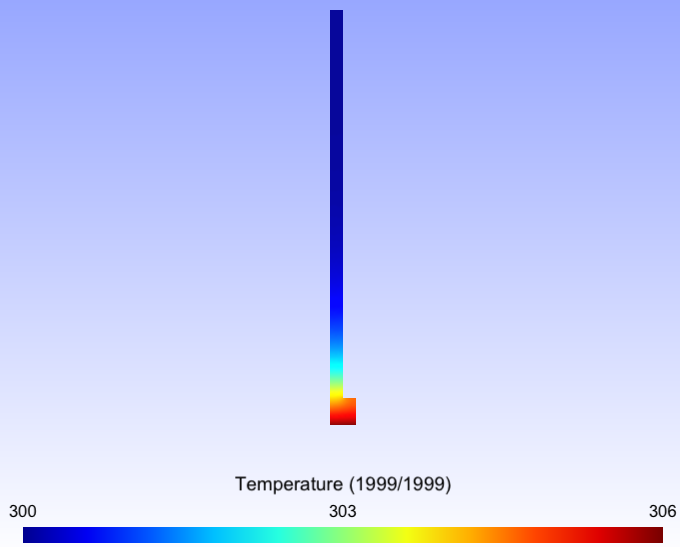
\includegraphics[width=1.7cm]{heatsink/heatsink_1.png}
%\end{minipage}
%\begin{minipage}[b]{.19\linewidth}
%\centering
%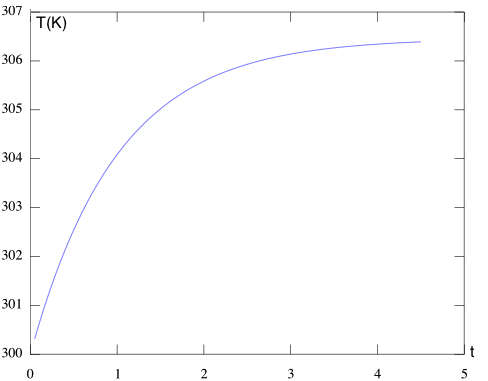
\includegraphics[width=1.7cm]{heatsink/heatsink_1_gamma4.png}
%\end{minipage}
%\begin{minipage}[b]{.19\linewidth}
%\centering
%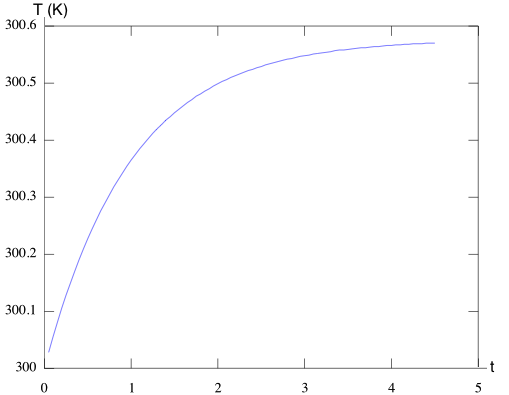
\includegraphics[width=1.7cm]{heatsink/heatsink_1_gamma1.png}
%\end{minipage}
%\end{figure}

\feelchapter{Natural convection in a heated tank}
            {Natural convection in a heated tank}
            {Christophe Prud'homme}
            {cha:natural-convection-2d}

\newcommand{\Gr}{\ensuremath{\mathrm{Gr}\xspace}}
\renewcommand{\Pr}{\ensuremath{\mathrm{Pr}\xspace}}

\section{Description}
\label{sec:description}

The goal of this project is to simulate the fluid flow under natural
convection: the heated fluid circulates towards the low temperature
under the action of density and gravity differences. Thie phenomenon
is important in the sense it models evacuation of heat, generated by
friction forces for example, with  a cooling fluid.

We shall put in place a simple convection problem in order to study
the phenomenon without having to handle the difficulties of more
complex domaines. We describe then some necessary transformations to
the equations, then we define quantities of interest to be able to
compare the simulations with different parameter values.


\newcommand{\Water}{\text{\textsc{Water}}\xspace}
\newcommand{\Fluid}{\text{\textsc{Fluid}}\xspace}
\tikzstyle{snakearrow} = [decoration={snake,aspect=0.2,segment length=1cm,amplitude=1mm},decorate]

\begin{figure}[htbp]
  \centering
  \begin{tikzpicture}[thick,scale=5]

    %% draw axis
    \draw[->] (-0.6,-0.4) -- (1.1,-0.4) node[right] {$x$} coordinate (x axis);
    \draw[-] (-0.,-0.39) -- (0,-0.41) node[below] {$0$};
    \draw[-] (1.,-0.39) -- (1,-0.41) node[below] {$W$};
    \draw[->] (-0.4,-0.6) -- (-0.4,1.1) node[above] {$y$} coordinate (y axis);
    \draw[-] (-0.39,-0.) -- (-0.41,-0.) node[left] {$0$};
    \draw[-] (-0.39,1.) -- (-0.41,1) node[left] {$1$};

    %% draw top and down walls
    \fill[pattern={north east lines},pattern color=blue] (0,1) rectangle  (1,1.02) ;
    \fill[pattern={north west lines},pattern color=blue] (0,0) rectangle  (1,-0.02) ;

    %% Draw the domain
    \draw[very thick,fill=blue!10!white,draw=blue!50] (0,0) rectangle  (1,1) ;
    \node at (0.1,0.5) {$\Gamma_1$};
    \node at (0.5,0.1) {$\Gamma_2$};
    \node at (0.9,0.5)  {$\Gamma_3$};
    \node at (0.8,0.9)  {$\Gamma_4$};
    \node (omega) at (0.5,0.3)  {$\Omega (\Fluid)$};
    % \draw[->,snakearrow] (omega) -- (0.5,0.5);
    \draw[<->] (0,-0.1) -- (1,-0.1) node [below,midway] {$W$};
    \draw[-] (0.5,1.) -- (0.5,0.5) node[left,midway] {$\Gamma_f$};
    \draw[-,ultra thick,color=blue] (0,0) -- (0,1) node [left,midway] {$T_0$};
    \draw[-,ultra thick,color=red] (1,0) -- (1,1)  {};


    \foreach \y in {0.1,0.3,0.5,0.7,0.9} {
      %%\draw[->] (\x, -1.5) -- (\x,\pgfmathqparse{-0.7*\x*\x+0.7*8*\x-12} \pgfmathresult);
      %%\pgfmathsetmacro{\pgf@x}{\x}
      %%\pgfmathparse{-0.7*\pgf@x*\pgf@x+0.7*8*\pgf@x-0.7*12}
      %%\def\y{\pgfmathresult}
      \def\x{1.3}
      \draw[->] (1.3, \y) -- (1.1,\y);
    }
    \node at (1.6,0.5) {Heat flux};

  \end{tikzpicture}
  \caption{Geometry of the model}
  \label{fig:heatns:1}
\end{figure}

To study the convection, we use a model problem: it consists in a
rectangular tank of height $1$ and width $W$, in which the fluid is
enclosed, see figure~\ref{fig:heatns:1}. We wish to know the fluid velocity
$\mathbf{u}$, the fluid pressure $p$ and fluid temperature $\theta$.

We introduce the adimensionalized Navier-Stokes and heat equations
parametrized by the Grashof and Prandtl numbers. These parameters
allow to describe the various regimes of the fluid flow and heat
transfer in the tank when varying them.

The adimensionalized steady incompressible Navier-Stokes equations reads:
\begin{equation}
  \label{eq:38}
  \begin{split}
    \mathbf{u}\cdot\nabla \mathbf{u} +\nabla p -\frac{1}{\sqrt{\Gr}} \Delta \mathbf{u} &= \theta \mathbf{e}_2\\
    \nabla \cdot \mathbf{u} & = 0\ \text{sur}\ \Omega\\
    \mathbf{u} & = \mathbf{0}\ \text{sur}\ \partial \Omega
  \end{split}
\end{equation}
where $\Gr$ is the Grashof number, $\mathbf{u}$ the adimensionalized
velocity and $p$ adimensionalized pressure and $\theta$ the
adimensionalized temperature. The temperature is in fact the
difference between the temperature in the tank and the temperature
$T_0$ on boundary $\Gamma_1$.

The heat equation reads:
\begin{equation}
  \label{eq:37}
  \begin{split}
    \mathbf{u} \cdot \nabla \theta -\frac{1}{\sqrt{\Gr}\Pr} \Delta \theta &= 0\\
    \theta &= 0\ \text{sur}\ \Gamma_1\\
    \frac{\partial \theta}{\partial n} &= 0\ \text{sur}\ \Gamma_{2,4}\\
    \frac{\partial \theta}{\partial n} &= 1\ \text{sur}\ \Gamma_3
  \end{split}
\end{equation}
where $\Pr$ is the Prandtl number.

% \section{Nombre de Grashof}
% \label{sec:nombre-de-grashof}
% Le nombre de Grashof (\Gr) est un nombre sans dimension utilisé en
% mécanique des fluides pour caractériser la convection libre dans un
% fluide. Il correspond au rapport des forces de gravité sur les forces
% visqueuses.

% On le définit de la manière suivante
% \begin{equation}
%   \label{eq:18}
%   \Gr = \frac{g\  \beta\  (T-T_\infty)\  {L_c}^3}{\nu^2}
% \end{equation}
% avec:
% \begin{itemize}
% \item $g$ - constante gravitationnelle
% \item $\beta$ - coefficient de dilatation
% \item $T-T_\infty$ - différence de température
% \item $L_c$ - longueur caractéristique
% \item $\nu$ - viscosité cinématique
% \end{itemize}

% \section{Nombre de Prandtl}
% \label{sec:nombre-de-prandtl}

% Le nombre de Prandtl (\Pr) est un nombre sans dimension. Il représente
% le rapport entre la diffusivité de quantité de mouvement $\nu$ (ou
% viscosité cinématique) et la diffusivité thermique.

% On le définit de la manière suivante
% \begin{equation}
%   \label{eq:19}
%   \Pr=\frac {\mu C_p }{\lambda}=\frac {\mu}{\frac {k}{C_p}}=\frac {\frac {\mu}{\rho}}{\frac {k}{\rho C_p}}=\frac {\nu}{\alpha}
% \end{equation}
% avec
% \begin{itemize}
% \item $\nu$ la viscosité cinématique en $m^2\cdot s^{-1}$
% \item $\rho$ la masse volumique en $kg\cdot m^{-3}$
% \item $\alpha$ la diffusivité thermique en $m^2\cdot s^{-1}$
% \item $\mu$ la viscosité dynamique en $N\cdot s\cdot m^{-2}$
% \item $C_p$ la chaleur massique en $J\cdot kg^{-1}\cdot K^{-1}$
% \item $k$ la conductivité thermique $W \cdot m^{-1}\cdot K^{-1}$
% \end{itemize}



\section{Influence of parameters}
\label{sec:infl-des-param}


what are the effects of the Grashof and Prandtl numbers ? We remark
that both terms with these parameters appear in front of the $\Delta$
parameter, they thus act on the diffusive terms. If we increase the
Grashof number or the Prandtl number the coefficients multiplying the
diffusive terms decrease, and this the convection, that is to say the
transport of the heat via the fluid, becomes dominant. This leads also
to a more difficult and complex flows to simulate, see
figure~\ref{fig:heatns:2}. The influence of the Grashof and Prandtl
numbers are different but they generate similar difficulties and flow
configurations. Thus we look only here at the influence of the Grashof
number which shall vary in $[1, 1e7]$.

\begin{figure}[htbp]
  \centering
  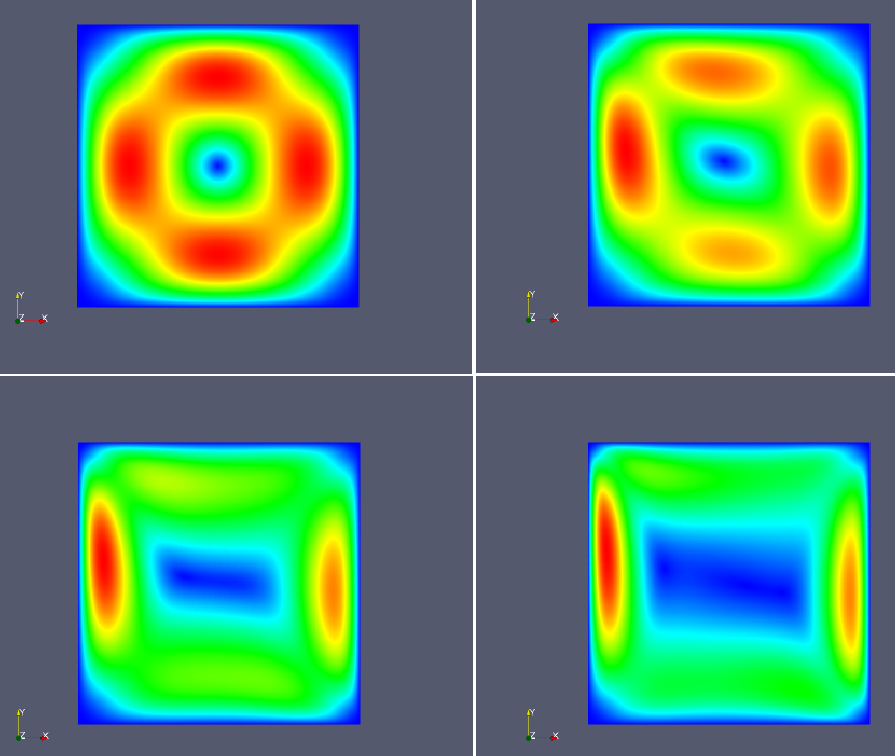
\includegraphics[width=.8\linewidth]{pngs/flow_grashof}
  \caption{Velocity norm with respect to  Grashof, $\Gr=100, 10000,
    100000, 500000$. $h=0.01$ and $\Pr=1$.}
  \label{fig:heatns:2}
\end{figure}

\section{Quantities of interest}
\label{sec:quant-du-benchm}

We would like to compare the results of many simulations with respect
to the Grashof defined in the previous section. We introduce two
quantities which will allow us to observe the behavior of the flow and
heat transfer.


\subsection{Mean temperature}
\label{sec:mean-temperature}

We consider first the mean temperature on boundary $\Gamma_3$
\begin{equation}
  \label{eq:16}
  T_3 = \int_{\Gamma_3} \theta
\end{equation}

This quantity should decrease with increasing Grashof because the
fluid flows faster and will transport more heat which will cool down
the heated boundary $\Gamma_3$. We observe this behavior on the
figure~\ref{fig:heatns:3}.

\begin{figure}[htbp]
  \centering
  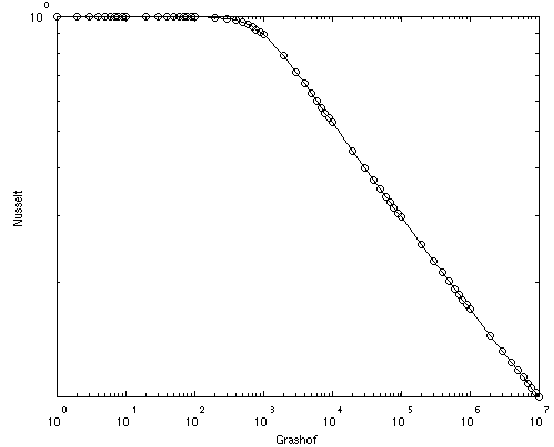
\includegraphics[width=.8\linewidth]{pngs/temp_grashof}
  \caption{Mean temperature with respect to the Grashof number;
    $h=0.02$ with $\mathbb{P}_3$ Lagrange element for the velocity,
    $\mathbb{P}_2$ Lagrange for the pressure and $\mathbb{P}_1$
    Lagrange for the temperature.}
  \label{fig:heatns:3}
\end{figure}

\subsection{Flow rate}
\label{sec:flow-rate}

Another quantity of interest is the flow rate through the middle of the
tank. We define a segment $\Gamma_f$ as being the vertical top
semi-segment located at $W/2$ with height $1/2$, see
figure~\ref{fig:heatns:1}. The flow rate, denoted $\mathrm{D}_f$, reads
\begin{equation}
  \label{eq:17}
  \mathrm{D}_f =  \int_{\Gamma_f} \mathbf{u} \cdot \mathbf{e}_1
\end{equation}
where $\mathbf{e}_1=(1,0)$. Note that the flow rate can be negative or
positive depending on the direction in which the fluid flows.

As a function of the Grashof, we shall see a increase in the flow
rate. This is true for small Grashof, but starting at $1e3$ the flow
rate decreases. The fluid is contained in a boundary layer which is
becoming smaller as the Grashof increases.

\begin{figure}[htbp]
  \centering
  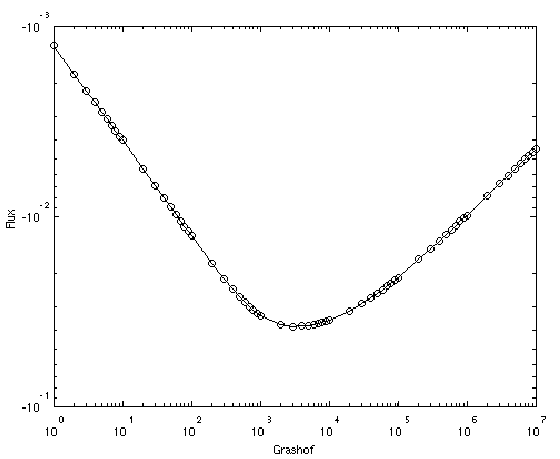
\includegraphics[width=.8\linewidth]{pngs/debit_grashof}
  \caption{Behavior of the flow rate with respect to the Grashof number; $h = 0.02$,
    $\mathbb{P}_3$ for the velocity, $\mathbb{P}_2$ for the pressure and
    $\mathbb{P}_1$ for the temperature.}
  \label{fig:4}
\end{figure}

\section{Implementation}
\label{sec:implementation}

This application in implemented in
\texttt{life/doc/tutorial/convection*.cpp}. The implementation solve
the full nonlinear problem using the nonlinear solver framework.

\section{Numerical Schemes}
\label{sec:numerical-schemes}

\subsection{Stokes problem formulation and the pressure}
\label{sec:stok-probl-form}

\subsection{The Stokes problem}
\label{sec:stokes-problem}

Consider the following problem,
\begin{equation}
  \label{notes:eq:16}
  \mbox{Stokes: }\left\{
    \begin{array}{rcc}
      -\mu\Delta\mathbf{u} +
      \nabla p =
      \mathbf{f}\\
      \nabla\cdot\mathbf{u} = 0\\
      \mathbf{u}|_{\partial \Omega} = 0
    \end{array}
  \right.
\end{equation}
where $\Omega \subset \mathbb{R}^d$. There are no boundary condition
on the pressure. This problem is ill-posed, indeed we only control the
pressure through its gradient $\nabla p$. Thus if $(\mathbf{u},p)$ is
a solution, then $(\mathbf{u},p+c)$ is also a solution with $c$ any
constant. This comes from the way the problem is posed: the box is
closed and it is not possible to determine the pressure inside. The
remedy is to impose arbitrarily a constraint on the pressure, e.g. its
mean value is zero. In other words, we add this new equation to the
problem (\ref{notes:eq:16})
\begin{equation}
  \label{notes:eq:17}
  \int_\Omega p = 0
\end{equation}
\begin{remark}[The Navier-Stokes case]
  This is also true for the incompressible Navier-Stokes equations. We
  chose Stokes to simplify the exposure.
\end{remark}

\subsection{Reformulation}
  In order to impose the condition~(\ref{notes:eq:17}), we introduce a new
  unknown, a Lagrange multiplier, $\lambda \in \mathbb{R}$ and modify
  the incompressibility equation. Our problem reads now, find
  $(\mathbf{u},p,\lambda)$ such
  that
    \begin{equation}
      \label{notes:eq:18}
    \mbox{Stokes 2: }\left\{
      \begin{array}{rcl}
        -\mu\Delta\mathbf{u} +
        \nabla p &=&
        \mathbf{f}\\
        \nabla\cdot\mathbf{u} + \lambda &=& 0\\
        \mathbf{u}|_{\partial \Omega} &=& 0\\
        \int_\Omega p &=& 0
      \end{array}
    \right.
\end{equation}
\begin{remark}[The pressure as Lagrange multiplier]
  The pressure field $p$ can actually be seen as a Lagrange multiplier
  for the velocity $\mathbf{u}$ in order to enforce the constraint
  $\nabla \cdot \mathbf{u} = 0$. $\lambda$ will play the same role but
  for the pressure to enforce the condition (\ref{notes:eq:17}). As $h
  \rightarrow 0$, $\lambda \rightarrow 0$ as well as the divergence of
  $\mathbf{u}$. Note also that $\int_\Omega \nabla \cdot \mathbf{u}
  \approx - \int_\Omega \lambda$ from the second equation.
\end{remark}

\subsection{Variational formulation}
\label{sec:vari-form}

The variational formulation now reads: find $(\mathbf{u}, p,
\lambda) \in \mathbf{H}^1_0(\Omega) \times L^2_0(\Omega) \times
\mathbb{R}$ such that for all $(\mathbf{v}, q, \eta) \in
\mathbf{H}^1_0(\Omega) \times L^2_0(\Omega) \times \mathbb{R}$

\begin{equation}
  \label{notes:eq:20}
  \mbox{Stokes 3: }\left\{
    \begin{array}{rcl}
      \int_\Omega \Big(\nabla \mathbf{u} \colon \nabla \mathbf{v} + \nabla \cdot \mathbf{v} p\Big) &=& \int_\Omega \mathbf{f} \cdot \mathbf{v}\\
      \int_\Omega \Big(\nabla\cdot\mathbf{u} q + \lambda q\Big)   &=& 0\\
      \int_\Omega p \eta &=& 0
    \end{array}
  \right.
\end{equation}

Summing up all three equations we get the following condensed formulation:

\begin{equation}
  \label{notes:eq:19}
  \int_\Omega \nabla \mathbf{u} \colon \nabla \mathbf{v} + \nabla \cdot \mathbf{v} p + \nabla \cdot \mathbf{u} q + \lambda q + \eta p = \int_\Omega \mathbf{f} \cdot \mathbf{v}
\end{equation}
where $\mathbf{H}^1_0(\Omega)= \Big\{ \mathbf{v} \in \mathbf{L}^2(\Omega), \nabla \mathbf{v} \in [L^2(\Omega)]^{d\times d},\ \mathbf{v} = 0\ \text{on}\ \partial \Omega \Big\}$,
$L^2_0(\Omega)= \Big\{ v \in L^2(\Omega),\ \int_\Omega v = 0\Big\}$, and
$\mathbf{L}^2(\Omega)= \Big\{ \mathbf{v} \in [L^2(\Omega)]^d\Big\}$ that is to say each component of a  vector field of $\mathbf{L}^2(\Omega)$ are in $L^2(\Omega)$.


\subsection{Implementation}
\label{sec:implementation}

  \begin{lstlisting}
/*basis*/
typedef Lagrange<Order, Vectorial> basis_u_type; // velocity
typedef Lagrange<Order-1, Scalar> basis_p_type; // pressure
typedef Lagrange<0, Scalar> basis_l_type; // multipliers
typedef bases<basis_u_type, basis_p_type, basis_l_type> basis_type;
/*space: product of the velocity, pressure and multiplier spaces*/
typedef FunctionSpace<mesh_type, basis_type, value_type> space_type;
// ...
space_ptrtype Xh = space_type::New( mesh );
element_type U( Xh, "u" );
element_type V( Xh, "v" );
element_0_type u = U.element<0>();
element_0_type v = V.element<0>();
element_1_type p = U.element<1>();
element_1_type q = V.element<1>();
element_2_type lambda = U.element<2>();
element_2_type nu = V.element<2>();
// ...
sparse_matrix_ptrtype D( M_backend->newMatrix( Xh, Xh ) );
form2( Xh, Xh, D, _init=true )=
   integrate( elements(mesh), im,
             // $\nabla \mathbf{u} \colon \nabla \mathbf{v}$
              mu*trace(deft*trans(def))
              // $\nabla \cdot \mathbf{v} p + \nabla \cdot \mathbf{u} q$
              - div(v)*idt(p) + divt(u)*id(q)
              // $\lambda q + \eta p$
              +id(q)*idt(lambda) + idt(p)*id(nu) );
// ...
  \end{lstlisting}


\subsection{Fix point iteration for Navier-Stokes}
\label{sec:fix-point-iteration}

\subsubsection{Steady incompressible Navier-Stokes equations}
  Consider the following steady incompressible Navier-Stokes
  equations, find $(\mathbf{u},p)$ such that
  \begin{equation}
    \label{notes:eq:7}
    \begin{split}
      \underbrace{\rho \mathbf{u} \cdot \nabla \mathbf{u}}_{\text{convection}} - \underbrace{\nu \Delta  \mathbf{u}}_{\text{diffusion}} + \nabla p &=  \mathbf{f} \ \text{on}\ \Omega \\
      \nabla \cdot \mathbf{u} &= 0 \\
      \mathbf{u} &= \mathbf{0}\ \text{on}\ \partial \Omega
    \end{split}
  \end{equation}
  where $\rho$ is the density of the fluid, $\nu$ is the dynamic
  viscosity of the fluid(la viscosité cinématique $\eta = \nu/\rho$) and $\mathbf{f}$ is the external force
  density applied to the fluid, (e.g. $\mathbf{f}=-\rho g \mathbf{e}_2$ with $\mathbf{e}_2=(0,1)^T$ ).  This equation system is nonlinear due
  to the $\mathbf{u} \cdot \nabla \mathbf{u}$ convection term. A
  simple approach to solve~(\ref{notes:eq:7}) is to use a fix point
  algorithm.


The fixpoint algorithm for NS reads as follows, find
$(\mathbf{u}^{(k)},p^{(k)})$ such that
    \begin{equation}
      \label{notes:eq:13}
    \begin{split}
      \rho\mathbf{u}^{(k-1)} \cdot \nabla \mathbf{u}^{(k)} - \nu \Delta  \mathbf{u}^{(k)} + \nabla p^{(k)} &= \mathbf{f} \ \text{on}\ \Omega \\
      \nabla \cdot \mathbf{u}^{(k)} &= 0 \\
      \mathbf{u}^{(k)} &= 0\ \text{on}\ \partial \Omega\\
      (\mathbf{u}^{(0)},p^{(0)}) &= (\mathbf{0},0)
    \end{split}
  \end{equation}
  The system~(\ref{notes:eq:13}) is now linear at each iteration $k$ and we
  can write the variational formulation accordingly. A stopping
  criterium is for example that
  $\|\mathbf{u}^{k}-\mathbf{u}^{(k-1)}\|+\|p^{k}-p^{(k-1)}\| <
  \epsilon$ where $\epsilon$ is a given tolerance (e.g. $1e-4$) and
  $\|\cdot\|$ is the $L_2$ norm.

  Here is the implementation using \Feel:

  \begin{lstlisting}
    // define some tolerance $\epsilon$
    epsilon = 1e-4;
    // set $(\mathbf{u}^{(0)},p^{(0)})$ to $(\mathbf{0},0)$
    velocity_element_type uk(Xh);
    velocity_element_type uk1(Xh);
    pressure_element_type pk(Ph);
    pressure_element_type pk1(Ph);
    // by default uk1, uk and pk,pk1 are initialized to 0

    // assemble the linear form associated to $\mathbf{f}$
    // store in vector $F$, it does not change over the iterations

    // iterations to find $(\mathbf{u}^{(k)},p^{(k)})$
    do
    {
      // save results of previous iterations
      uk1 = uk;
      pk1 = pk;

      //assemble for bilinear form  associated to
      // $\rho\mathbf{u}^{(k-1)} \cdot \nabla \mathbf{u}^{(k)} - \nu \Delta  \mathbf{u}^{(k)} + \nabla p^{(k)}$
      // store in matrix $A^{(k)}$

      // solve the system $A^{(k)} X = F$ where $X = (\mathbf{u}^{(k)},p^{(k)})^T$

      // use uk,uk1 and pk,pk1 to compute the error estimation at each iteration
      error = $\|\mathbf{u}^{k}-\mathbf{u}^{(k-1)}\|+\|p^{k}-p^{(k-1)}\|$
    } while( error > epsilon );

  \end{lstlisting}

\subsection{A Fix point coupling algorithm}
\label{sec:coupling-algorithm}

\subsubsection{Coupling fluid flow and heat transfer: problem}
  Recall that we have to solve two coupled problems :

  $$
  \mbox{Heat(\textbf{u}) }\left\{
  \begin{array}{rcc}
    - \kappa\Delta T + \mathbf{u}\cdot\nabla T &=& 0 \\
    T|_{\Gamma_1} &=& T_0 \\
    \frac{\partial T}{\partial \mathbf{n}}|_{\Gamma_3} &=&1 \\
    \frac{\partial T}{\partial \mathbf{n}}|_{\Gamma_2,\Gamma_4} &=& 0
  \end{array}
  \right.
  $$

  and

  $$\mbox{Stokes(T) : }\left\{
    \begin{array}{rcc}
      -\nu\Delta\mathbf{u} +
      \frac{1}{\rho}\nabla p =
      \mathbf{F}\\
      \nabla\cdot\mathbf{u} = 0\\
      \mathbf{u}|_{\partial \Omega} = 0
    \end{array}
  \right.
  $$

Where $\mathbf{F}$ can be taken as $
 \left(
  \begin{array}{c}
    0 \\
    \beta(T-T_0)
  \end{array}
\right)
$
for some $\beta > 0$. $\beta$ is called the \emph{dilatation coefficient}.

\subsubsection{Coupling fluid flow and heat transfer: algorithm}
Here is a simple algorithm fix point strategy in pseudo-code:
\begin{lstlisting}
   double tol = 1.e-6;
   int maxIter = 50;
   //Initial guess Un = 0
   do
   {
     // Find Tn solution of Heat(Un)
     // Find Unp1 solution of Stokes(Tn)
     // compute stopTest = norme(Unp1 - Un)
     // Un = Unp1
   }while((stopTest < tol) && (niter <= maxIter));
\end{lstlisting}

\begin{remark}[The unsteady case]
  To solve the unsteady problems, one can insert the previous loop in
  the one dedicated to time discretization
\end{remark}

\subsection{A Newton coupling algorithm}
\label{sec:newt-coupl-algor}

\subsubsection{A fully coupled scheme}

  Another possiblity is to use a Newton method which allows us to
  solve the full nonlinear problem coupling velocity, pressure and
  temperature
  \begin{equation}
    \label{notes:eq:21}
    \text{Find}\ X\ \text{such that}\ F(X) = 0
  \end{equation}
  the method is iterative and reads, find $X^{(n+1)}$ such that
  \begin{equation}
    \label{notes:eq:22}
    J_F(X^{(n)})( X^{(n+1)}-X^{(n)}) = - F (X^{(n)})
  \end{equation}
  starting with $X^{(0)} = \mathbf{0}$ or some other initial value and
  where $J_F$ is the jacobian matrix of $F$ evaluated at
  $X=((u_i)_i,(p_i)_i,(\theta_i)_i)^T$.  For any $\phi_k, \psi_l$ and
  $\rho_m$ the \emph{test} functions associated respectively to velocity,
  pressure and temperature, our full system reads, Find $X=((u_i)_i,(p_i)_i,(\theta_i)_i)^T$ such that
  \begin{equation}
    \label{notes:eq:23}
    \begin{array}{rll}
      F_1((u_i)_i,(p_i)_i,(\theta_i)_i)&=\sum_{i,j} u_i u_j a(\phi_i,\phi_k,\phi_j) - \sum_i p_i b(\phi_k,\psi_i) + \sum_i \theta_i c(\rho_i, \phi_k)+\sum_i u_i d(\phi_i,\phi_k)  &= 0\\
      F_2((u_i)_i,(p_i)_i,(\theta_i)_i)&=\sum_i u_i b(\phi_i,\psi_l) &=0\\
      F_3((u_i)_i,(p_i)_i,(\theta_i)_i)&=\sum_{i,j} u_i\theta_j e(\phi_i,\rho_j,\rho_m) + \sum_i \theta_i f(\rho_i,\rho_m)-g(\rho_m) &=  0
    \end{array}
  \end{equation}
  where $F=(F_1,F_2,F_3)^T$ and
  \begin{equation}
    \label{notes:eq:26}
    \begin{array}{rl}
    a(\mathbf{u},\mathbf{v},\beta) &= \int_\Omega \mathbf{v}^T ((\nabla \mathbf{u} )\beta)\\
    b(\mathbf{v},p) &= \int_\Omega p (\nabla \cdot \mathbf{v}) - \int_{\partial \Omega} \mathbf{v}\cdot\mathbf{n} p\\
      c(\theta,\mathbf{v})&= \int_\Omega \theta \mathbf{e}_2 \cdot \mathbf{v}\\
      d(\mathbf{u},\mathbf{v}) &= \frac{1}{\sqrt{\mathrm{Gr}}} \Big(\int_\Omega \nabla \mathbf{u} \colon (\nabla \mathbf{v})^T - \int_{\partial \Omega} ((\nabla \mathbf{u}) \mathbf{n})\cdot \mathbf{v}\Big)\\
      e(\mathbf{u},\theta,\chi) &= \int_\Omega (\mathbf{u}\cdot \nabla \theta) \chi \\
      f(\theta,\chi) &=\frac{1}{\sqrt{\mathrm{Gr}}\mathrm{Pr}} \Big( \int_\Omega \nabla \theta \cdot \nabla \chi - \int_{\Gamma_1} (\nabla \theta \cdot \mathbf{n} ) \chi \Big)\\
      g(\chi) &=\frac{1}{\sqrt{\mathrm{Gr}}\mathrm{Pr}} \int_{\Gamma_3} \chi
    \end{array}
  \end{equation}
  \begin{remark}
    Note that the boundary integrals are kept in order to apply the
    weak Dirichlet boundary condition trick, see next section~\ref{sec:weak-dirichl-boud}.
  \end{remark}

\subsubsection{Jacobian matrix}
  In order to apply the newton scheme, we need to compute the jacobian
  matrix $J_F$ by deriving each equation with respect to each
  unknowns, ie $u_i, p_i$ and $\theta_i$.
  Consider the first equation
  \begin{itemize}
  \item Deriving the first equation with respect to $u_i$ we get
    \begin{equation}
      \label{notes:eq:30}
      \frac{\partial F_1}{\partial u_i} = \sum_j u_j a(\phi_i,\phi_k,\phi_j) + \sum_i u_i a(\phi_i,\phi_k,\phi_j) + d(\phi_i,\phi_k)
    \end{equation}
  \item Deriving the first equation with respect to $p_i$ we get
    \begin{equation}
      \label{notes:eq:30}
      \frac{\partial F_1}{\partial p_i} =  -b(\phi_k,\psi_l)
    \end{equation}
  \item Deriving the first equation with respect to $\theta_i$ we get
    \begin{equation}
      \label{notes:eq:30}
      \frac{\partial F_1}{\partial \theta_i} = c(\rho_i,\rho_k)
    \end{equation}

  \end{itemize}
  Consider the second equation, only the derivative with respect to $u_i$ is non zero.
  \begin{equation}
    \label{notes:eq:31}
    \frac{\partial F_2}{\partial u_i} = b(\phi_i,\psi_l)
  \end{equation}
  Finally the third component
  \begin{itemize}
  \item Deriving with respect to $u_i$
    \begin{equation}
      \label{notes:eq:33}
      \frac{\partial F_3}{\partial u_i} = \sum_j \theta_j e(\phi_i,\rho_j,\rho_m)
    \end{equation}
  \item Deriving with respect to $p_i$,
    \begin{equation}
      \label{notes:eq:34}
      \frac{\partial F_3}{\partial p_i} = 0
    \end{equation}
  \item Deriving with respect to $theta_i$,
    \begin{equation}
      \label{notes:eq:35}
      \frac{\partial F_3}{\partial \theta_i} = \sum_j u_j e(\phi_j,\rho_i,\rho_m) + f(\rho_i,\rho_m)
    \end{equation}
  \end{itemize}
  \begin{equation}
    \label{notes:eq:35}
    J_F =
    \begin{pmatrix}
      \frac{\partial F_1}{\partial u_i} & \frac{\partial F_1}{\partial p_i} & \frac{\partial F_1}{\partial \theta_i} \\
      {\frac{\partial F_2}{\partial u_i}} & {\frac{\partial F_2}{\partial p_i}}(=0) & {\frac{\partial F_2}{\partial \theta_i}}(=0) \\
      \frac{\partial F_3}{\partial u_i} & {\frac{\partial F_3}{\partial p_i}}(=0) & \frac{\partial F_3}{\partial \theta_i}
    \end{pmatrix}
  \end{equation}
  In order to implement $J_F$ and solve (\ref{notes:eq:22}), $J_F$ can be
  expressed as the matrix associated with the discretisation of
  \begin{equation}
    \label{notes:eq:37}
    \begin{array}{rl}
      a(\mathbf{u},\mathbf{v},\beta_1) + a(\beta_1, \mathbf{v}, \mathbf{u})+d(\mathbf{u},\mathbf{v})-b(\mathbf{v},p)+c(\theta,\mathbf{v}) &= 0\\
      b(\mathbf{u},q)&=0\\
      e(\beta_1,\theta,\chi)+f(\theta,\chi)+e(\mathbf{u},\beta_2,\chi)&=0\\
    \end{array}
  \end{equation}
  where $\beta_1 = u^{(n)}$, $\beta_2=\theta^{(n)}$ are known from the
  previous Newton iteration, indeed $J_F$ is actually evaluated in $X^{(n)}$.

\subsubsection{\Feel Implementation}
  Now we use the \Feel non linear framework in order to implement our
  Newton scheme~(\ref{notes:eq:22}).
  We need to define two new functions in our application
  \begin{itemize}
  \item \texttt{updateJacobian(X,J)} which takes as input \texttt{X}$=X^{(n)}$ and returns the matrix \texttt{J=}$J_F(X^{(n)})$
  \item \texttt{updateResidual(X,R)} which takes as input \texttt{X}$=X^{(n)}$ and returns the vector \texttt{R=}$F(X^{(n)})$
  \end{itemize}

  \begin{remark}{Backend}
    Only the PETSC backend supports the nonlinear solver framework.
    Use  in the command line like in the first section
    \begin{lstlisting}
      --backend=petsc
    \end{lstlisting}
  \end{remark}

  Here is a snippet of code that implements the nonlinear framework.
  \begin{lstlisting}
    class MyApp
    {
      public:
      void run();
      void updateResidual( const vector_ptrtype& X, vector_ptrtype& R );
      void updateJacobian( const vector_ptrtype& X, sparse_matrix_ptrtype& J);
      void solve( sparse_matrix_ptrtype& D, element_type& u, vector_ptrtype& F );
      private:

      backend_ptrtype M_backend;
      sparse_matrix_ptrtype M_jac;
      vector_ptrtype M_residual;
    };

    void
    MyApp::run()
    {
      // ...

      // plug the updateResidual and updateJacobian functions
      // in the nonlinear framework
      M_backend->nlSolver()->residual = boost::bind( &self_type::updateResidual,
                                                     boost::ref( *this ), _1, _2 );
      M_backend->nlSolver()->jacobian = boost::bind( &self_type::updateJacobian,
                                                     boost::ref( *this ), _1, _2 );

      vector_ptrtype U( M_backend->newVector( u.functionSpace() ) );
      *U = u;
      vector_ptrtype R( M_backend->newVector( u.functionSpace() ) );
      this->updateResidual( U, R );
      sparse_matrix_ptrtype J;
      this->updateJacobian( U, J );
      solve( J, u, R );

      *U = u;
      this->updateResidual( U, R );
      // R(u) should be small
      std::cout << "R( u ) = " << M_backend->dot( U, R ) << "\n";


    }
    void
    MyApp::solve( sparse_matrix_ptrtype& D, element_type& u, vector_ptrtype& F )
    {
      vector_ptrtype U( M_backend->newVector( u.functionSpace() ) );
      *U = u;
      M_backend->nlSolve( D, U, F, 1e-10, 10 );
      u = *U;
    }
    void
    MyApp::updateResidual( const vector_ptrtype& X, vector_ptrtype& R )
    {
      // compute R(X)

      R=M_residual;
    }
    void
    MyApp::updateJacobian( const vector_ptrtype& X, vector_ptrtype& R )
    {
      // compute J(X)

      J=M_jac;
    }
  \end{lstlisting}
  see \texttt{bratu.cpp} or \texttt{nonlinearpow.cpp} for example.


%%% Local Variables:
%%% coding: utf-8
%%% mode: latex
%%% TeX-PDF-mode: t
%%% TeX-parse-self: t
%%% x-symbol-8bits: nil
%%% TeX-auto-regexp-list: TeX-auto-full-regexp-list
%%% TeX-master: "../feel-manual"
%%% ispell-local-dictionary: "american"
%%% End:


\feelchapter{2D Maxwell simulation in a diode}
            {2D Maxwell simulation in a diode}
            {Thomas Strub, Philippe Helluy, Christophe Prud'homme}
            {cha:maxwell-2d}

\section{Description}
\label{sec:description}

\begin{itemize}
\item applications
\item geometry
\item
\end{itemize}

\section{Variational formulation}
\label{sec:vari-form}

\section{Implementation}
\label{sec:implementation}

\section{Numerical Results}
\label{sec:numerical-results}


%%% Local Variables:
%%% coding: utf-8
%%% mode: latex
%%% TeX-PDF-mode: t
%%% TeX-parse-self: t
%%% x-symbol-8bits: nil
%%% TeX-auto-regexp-list: TeX-auto-full-regexp-list
%%% TeX-master: "../feel-manual"
%%% ispell-local-dictionary: "american"
%%% End:

\feelchapter{Domain decomposition methods}
            {Domain decomposition methods}
            {Abdoulaye Samake, Vincent Chabannes, Christophe Prud'homme}
            {cha:dd}

\section{A Really Short Introduction}
\label{sec:really-short-intr}
In mathematics, numerical analysis, and numerical partial differential equations, domain decomposition methods solve
a boundary value problem by splitting it into smaller boundary value problems on subdomains and iterating to coordinate
the solution between the adjacent subdomains. A corse problem with one or fiew unknows per subdomain is used to further
coordinate the solution between the subdomains globally.
\section{A 1D model}
\label{sec:1d-mode}
We consider the following laplacian boundary value problem
\begin{equation}
  \left \{
    \begin{aligned}
      & -u"(x) = f(x) \quad \text{in} \quad  ]0,1[ \\
      & u(0) =\alpha, ~ u(1) = \beta
    \end{aligned}
  \right.
\label{eq:30}
\end{equation}
where $\alpha, \beta \in \mathbb R.$
\subsection{Schwartz algorithms}
\label{sec:schwartz-algorithms}
The schwartz overlapping multiplicative algorithm with dirichlet interface conditions for this problem at $n^{th}$ iteration is given by
\begin{equation}
  \label{eq:31}
  \left \{
    \begin{aligned}
      -u_1"^n(x) & =  f(x) \quad  \text{in}  \quad  ]0,b[  \\
       u_1^n(0) & =  \alpha \\
       u_1^n(b)  & = u_2^{n-1}(b)
    \end{aligned}
  \right.
\qquad \text{and} \qquad
  \left \{
    \begin{aligned}
      -u_2"^n(x) & =  f(x) \quad  \text{in}  \quad  ]a,1[  \\
      u_2^n(1) & =  \beta \\
      u_2^n(a)  & = u_1^n(a)
    \end{aligned}
  \right.
\end{equation}
where $ n \in \mathbb N^*, a, b \in \mathbb R $ and $a < b$. \\
Let $e_i^n = u_i^n-u~(i=1,2)$, the error at $n^{th}$ iteration relative to the exact solution, the convergence rate is given by
\begin{equation}
  \rho = \frac{\vert e_1^n  \vert}{\vert e_1^{n-1}  \vert} = \frac{a}{b}\frac{1-b}{1-a} = \frac{\vert e_2^n  \vert}{\vert e_2^{n-1}  \vert} .
  \label{eq:32}
\end{equation}

\subsection{Variational formulations}
\label{sec:vari-form-1}
find $u$ such that
\begin{equation*}
  \int_0^b u_1'v' = \int_0^b fv \quad \forall v \qquad \text{in the first subdomain} ~\Omega_1 = ]0,b[
\end{equation*}
\vspace{-5pt}
\begin{equation*}
  \int_a^1 u_2'v' = \int_a^1 fv \quad \forall v \qquad \text{in the second subdomain} ~ \Omega_2 = ]a,1[
\end{equation*}

\section{A 2 domain overlapping Schwartz method in 2D and 3D}
\label{sec:2-doma-overl}

We consider the following laplacian boundary value  problem
\begin{equation}
  \left \{
    \begin{aligned}
      -\Delta u & = f \quad \text{in} \quad  \Omega \\
      u & = g \quad \text{on} \quad  \partial\Omega
    \end{aligned}
  \right.
 \label{eq:33}
\end{equation}
where $\Omega \subset \mathbb R^d, d=2,3$ and $g$ is the dirichlet boundary value.

\subsection{Schwartz algorithms}
\label{sec:schwartz-algorithms-1}
The schwartz overlapping multiplicative algorithm with dirichlet interface conditions for this problem on two subdomains $\Omega_1$
and $\Omega_2$ at $n^{th}$ iteration is given by
\begin{equation}
  \label{eq:34}
  \left \{
    \begin{aligned}
      -\Delta u_1^n & =  f \quad \qquad  \text{in}  \quad  \Omega_1  \\
       u_1^n  & =  g \quad \qquad  \text{on} \quad \partial \Omega_1^{ext}\\
       u_1^n  & = u_2^{n-1} \quad ~~  \text{on} \quad \Gamma_1
    \end{aligned}
  \right.
\qquad \text{and} \qquad
  \left \{
    \begin{aligned}
      - \Delta u_2^n & =  f \quad \qquad  \text{in}  \quad  \Omega_2  \\
      u_2^n  & =  g  \quad \qquad  \text{on} \quad \partial \Omega_2^{ext}\\
      u_2^n  & = u_1^n \qquad~~  \text{on} \quad \Gamma_2
    \end{aligned}
  \right.
\end{equation}

\subsection{Variational formulations}
\label{sec:vari-form-2}

\begin{equation*}
  \begin{aligned}
    \int_{\Omega_i} \nabla u_i \cdot \nabla v = \int_{\Omega_i} fv   \quad \forall~ v,~i=1,2.
  \end{aligned}
\end{equation*}

\subsubsection{\FEEL implementation}
\label{sec:feel-implementation}
\begin{lstlisting}
/*
  Implementation of the local problem
*/
template<Expr>
void
localProblem(element_type& u, Expr expr)
{
 // Assembly of the right hand side $ \mathlarger \int_\Omega fv $
    auto F = M_backend->newVector(Xh);
    form1( _test=Xh,_vector=F, _init=true ) =
           integrate( elements(mesh), f*id(v) );
    F->close();

 // Assembly of the left hand side $ \mathlarger \int_\Omega \nabla u \cdot  \nabla v$
    auto A = M_backend->newMatrix( Xh, Xh );
    form2( _test=Xh, _trial=Xh, _matrix=A, _init=true ) =
           integrate( elements(mesh), gradt(u)*trans(grad(v)) );
    A->close();

 // Apply the dirichlet boundary conditions
    form2( Xh, Xh, _matrix=A ) +=
           on( markedfaces(mesh, "Dirichlet") ,u,F,g);

 // Apply the dirichlet interface conditions
    form2( Xh, Xh, _matrix=A ) +=
           on( markedfaces(mesh, "Interface") ,u,F,expr);

 // solve the linear system $ A u = F $
    M_backend->solve(_matrix=A, _solution=u, _rhs=F );
}

  unsigned int cpt = 0;
  double tolerance = $1e-8$;
  double maxIterations = 20;
  double l2erroru$_1$ = 1.;
  double l2erroru$_2$ = 1;
  /*
  Iteration loop
  */
  while( (l2erroru$_1$ +l2erroru$_2$) > tolerance && cpt <= maxIterations)
  {

    // call the localProblem on the first subdomain $\Omega_1$
       localProblem(u$_1$, idv(u$_2$));

    // call the localProblem on the first subdomain $\Omega_2$
       localProblem(u$_2$, idv(u$_1$));

    // compute L2 errors on each subdomain
       L2erroru$_1$ = l2Error(u$_1$);
       L2erroru$_2$ = l2Error(u$_2$);

    // increment the cunter
        ++cpt;
  }

\end{lstlisting}

\subsection{Numerical results in 2D case}
\label{sec:numerical-results-1}
The numerical results presented in the following table correspond to the partition of the global domain $\Omega$ in two subdomains $\Omega_1$ and $\Omega_2$~(see figure \ref{fig:original}) and the following configuration:
\begin{enumerate}
\item $ g(x,y) = \sin(\pi x)\cos(\pi y)$~:~ the exact solution
\item $f(x,y) = 2\pi^2g$~:~ the right hand side of the equation
\item $\mathbb P_2$ approximation~:~ the lagrange polynomial order
\item hsize $= 0.02$~:~ the mesh size
\item tol $=1e-9$~:~ the tolerance
\end{enumerate}

\begin{figure}[htbp]
  \centering
  \subfigure[Two overlapping subdomains]{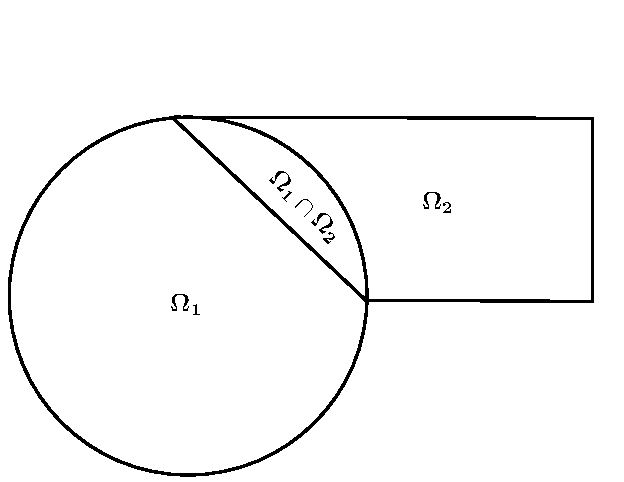
\includegraphics[width=.40\linewidth]{dd2dgeometry.pdf}}
  \hspace{0.25cm}
  \subfigure[Two overlapping meshes]{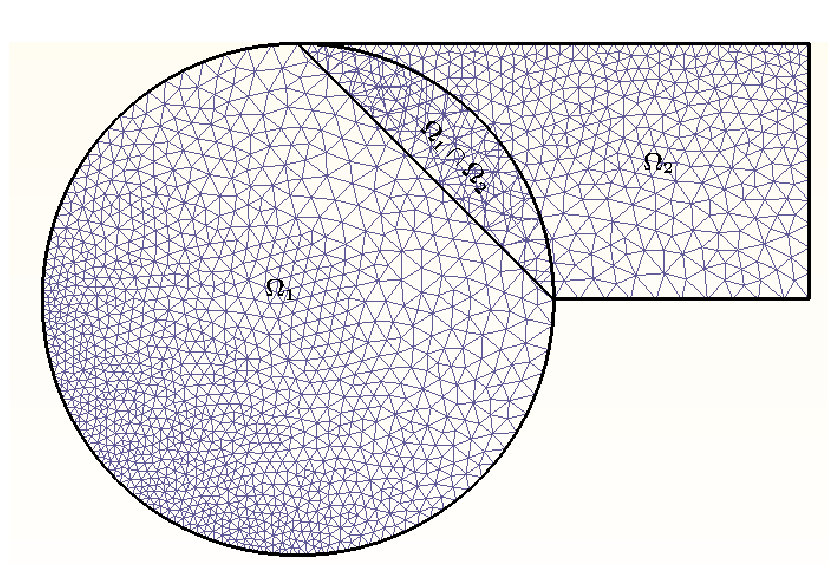
\includegraphics[width=.38\linewidth]{dd2dmesh.pdf}}
  \caption{geometry}
  \label{fig:original}
\end{figure}

\vspace{0.3cm}
\begin{center}
  \begin{tabular}{|c|c|c|}
  \hline
   \textbf{Nomber of iterations} & $\mathbf {\| u_1-u_{ex}\|_{L_2} }$ & $\mathbf{\| u_2-u_{ex}\|_{L_2}}$ \\
   \hline
    11 & 2.52e-8 & 2.16e-8 \\
   \hline
 \end{tabular}
\end{center}
% \begin{center}
% \begin{tabular}{|c|c|c|c|}
%   \hline
%   \textbf{Overlap} & \textbf{Nomber of iterations} & $\mathbf {\| u_1-u_{ex}\|_{L_2} }$ & $\mathbf{\| u_2-u_{ex}\|_{L_2}}$ \\
%   \hline
%    0 & -  & - & - \\
%   \hline
%   0.25 & 11 & 2.52e-8 & 2.16e-8 \\
%   \hline
%   0.50 & 8 & 2.34e-8 & 2.34e-8 \\
%   \hline
%   0.75 & 5 & 2.16e-8 & 2.31e-8 \\
%   \hline
%   1 & 2 & 2.11e-8 & 2.09e-8 \\
%   \hline
% \end{tabular}
% \end{center}
\vspace{0.2cm}
\subsection{Numerical solutions in 2D case}
\label{sec:numerical-solutions}
%$\Big \Omega_1$
% \begin{figure}[htbp]
% \centering
% \includegraphics[width=.5\linewidth]{dd2d.pdf}
%   \caption{The two overlapping meshes }
%   \label{fig:14}
% \end{figure}
\begin{figure}[htbp]
  \centering
  \subfigure[first iteration]{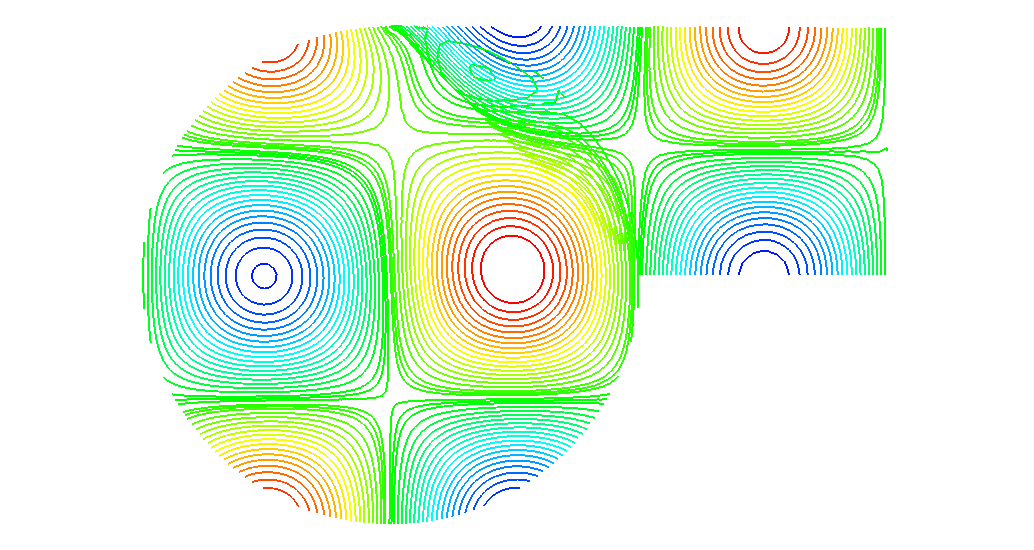
\includegraphics[width=.48\linewidth]{iter_1.png}}
  \subfigure[$10^{th}$ iteration]{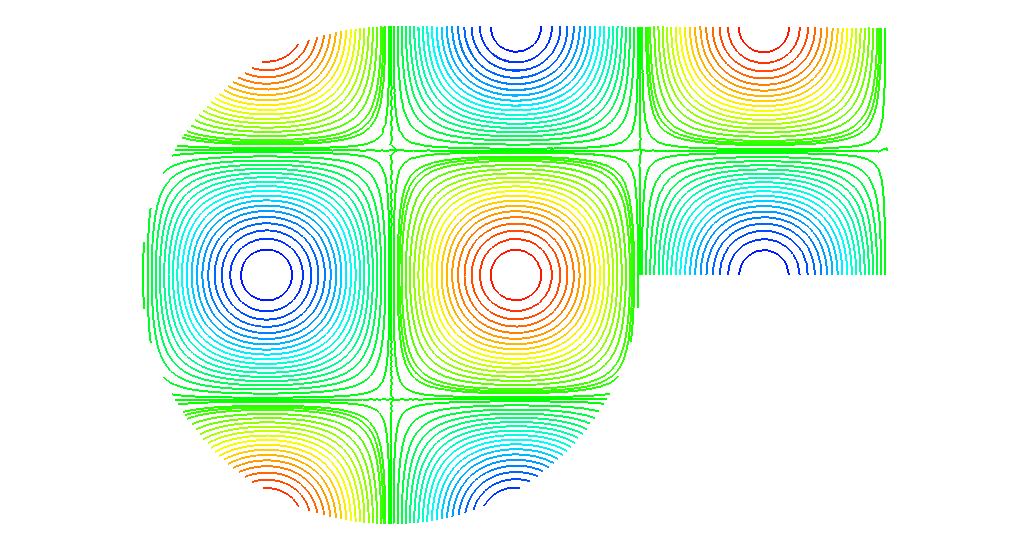
\includegraphics[width=.48\linewidth]{iter_10.png}}
  \caption{isovalues of solution in 2D}
  \label{fig:original}
\end{figure}


\section{Computing the eigenmodes of the Dirichlet to Neumann operator}
\label{sec:comp-eigenm-dirichl}

\subsection{Problem description and variational formulation}
\label{sec:probl-descr-vari}

We consider at the continuous level the Dirichlet-to-Neumann(DtN) map on $\Omega$, denoted by DtN$_{\Omega}$.

Let $u: \Gamma \longmapsto \mathbb R, $
\begin{equation*}
  \label{eq:35}
\text{DtN}_{\Omega}(u) = \kappa \frac{\partial v}{ n} \Big |_{\Gamma}
\end{equation*}
where $v$ satisfies
\begin{equation}
  \label{eq:36}
\left\{
  \begin{aligned}
    & \mathcal L(v):= (\eta - \text{div}(\kappa \nabla))v = 0 & \text{dans} \quad \Omega,\\
    & v = u & \text{sur} \quad \Gamma
  \end{aligned}
\right.
\end{equation}

where $\Omega$ is a bounded domain of $\mathbb R^d$ (d=2 or 3), and $\Gamma$ it border, $\kappa$ is a positive
diffusion function which can be discontinuous, and $\eta \geq 0$. The eigenmodes of the Dirichlet-to-Neumann
operator are solutions of the following eigenvalues problem
\begin{equation}
  \label{eq:37}
  \text{DtN}_{\Omega}(u) = \lambda \kappa u
\end{equation}
To obtain the discrete form of the DtN map, we consider the variational form of (\ref{eq:36}). let's define the
bilinear form $a~:~H^1(\Omega) \times H^1(\Omega) \longrightarrow \mathbb R $,
\begin{equation*}
  \label{eq:41}
  a(w,v) := \int_\Omega \eta w v + \kappa \nabla w \cdot \nabla v .
\end{equation*}
With a finite element basis $\{ \phi_k \}$, the coefficient matrix of a Neumann boundary value problem in $\Omega$ is
\begin{equation*}
\label{eq:42}
  A_{kl} := \int_\Omega \eta \phi_k \phi_l + \kappa \nabla \phi_k \cdot \nabla \phi_l .
\end{equation*}
A variational formulation of the flux reads
\begin{equation*}
  \label{eq:43}
\int_\Gamma \kappa \dfrac{\partial v}{\partial n} \phi_k = \int_\Omega \eta v \phi_k + \kappa \nabla v \cdot \nabla \phi_k \quad \forall~ \phi_k.
\end{equation*}
So the variational formulation of the eigenvalue problem (\ref{eq:37}) reads
\begin{equation}
\label{eq:40}
 \int_\Omega \eta v \phi_k + \kappa \nabla v \cdot \nabla \phi_k = \lambda \int_\Gamma \kappa v \phi_k  \quad \forall~ \phi_k.
\end{equation}
Let $B$ be the weighted mass matrix
\begin{equation*}
  \label{eq:44}
  (B)_{kl} = \int_\Gamma \kappa \phi_k \phi_l
\end{equation*}
The compact form of (\ref{eq:40}) is
\begin{equation}
  \label{eq:45}
  Av = \lambda B v
\end{equation}

\subsubsection{\FEEL implementation}
\label{sec:feel-implementation-1}

\begin{lstlisting}

// Assembly of the right hand side $ B = \mathlarger \int_\Gamma \kappa v w $
 auto B = M_backend->newMatrix( Xh, Xh ) ;
 form2( _test=Xh, _trial=Xh, _matrix=B, _init=true );
 BOOST_FOREACH( int marker, flags )
 {
   form2( Xh, Xh, _matrix=B ) +=
   integrate( markedfaces(mesh,marker), kappa*idt(u)*id(v) );
 }
 B->close();
// Assembly of the left hand side $ A = \mathlarger \int_\Omega \eta v w + \kappa \nabla v \cdot \nabla w $
 auto A = M_backend->newMatrix( Xh, Xh ) ;
 form2( _test=Xh, _trial=Xh, _matrix=A, _init=true ) =
 integrate( elements(mesh), kappa*gradt(u)*trans(grad(v)) + nu*idt(u)*id(v) );
 A->close();

// eigenvalue solver options
 int nev = this->vm()["solvereigen-nev"].template as<int>();
 int ncv = this->vm()["solvereigen-ncv"].template as<int>();;
// definition of the eigenmodes
 SolverEigen<double>::eigenmodes_type modes;
// solve the eigenvalue problem $ Av =  \lambda B v $
 modes=
       eigs( _matrixA=A,
             _matrixB=B,
             _nev=nev,
             _ncv=ncv,
             _transform=SINVERT,
             _spectrum=SMALLEST_MAGNITUDE,
             _verbose = true );

}

\end{lstlisting}

\subsection{Numerical solutions}
\label{sec:numerical-solutions-1}
\vspace{-17pt}
\begin{figure}[htbp]
  \centering
  \subfigure[first mode]{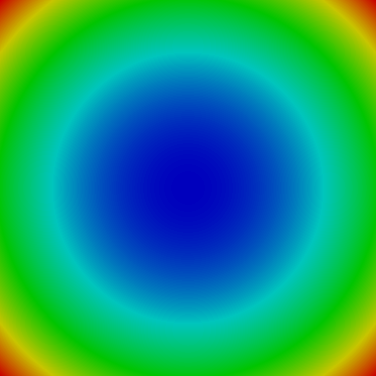
\includegraphics[width=.24\linewidth]{mode-0}}
  \hspace{0.3cm}
  \subfigure[second mode]{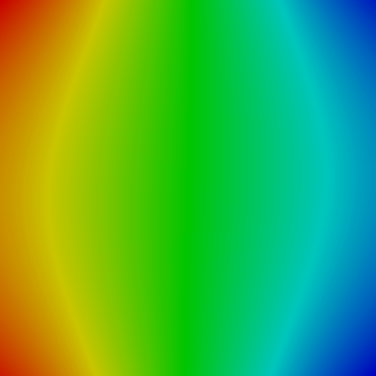
\includegraphics[width=.24\linewidth]{mode-1}}
  \hspace{0.3cm}
  \subfigure[third mode]{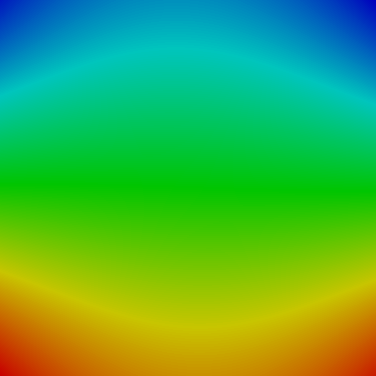
\includegraphics[width=.24\linewidth]{mode-2}}
  \caption{three eigenmodes}
\label{fig:eigenvalues}
\end{figure}
These numerical solutions correspond to the following configuration :
\begin{enumerate}
\item $\mathbb P_2$ approximation~:~ the lagrange polynomial order
\item hsize $= 0.02$~:~ the mesh size
\item $\mu = \kappa = 1.$
\end{enumerate}
%%% Local Variables:
%%% coding: utf-8
%%% mode: latex
%%% TeX-PDF-mode: t
%%% TeX-parse-self: t
%%% x-symbol-8bits: nil
%%% TeX-auto-regexp-list: TeX-auto-full-regexp-list
%%% TeX-master: "../feel-manual"
%%% ispell-local-dictionary: "american"
%%% End:

%\include{examples/heat-transfer}
%\include{examples/solid-mechanics}

\part{Programming with \feel}
%\include{developer/}


%_______        ANNEXES / APPENDIX      ________
\part{Appendix}
\appendix

\chapter{How to ?}
\label{sec:faq}

\section{Introduction}
\label{faq:intro}

This section includes the FAQ avaible on \href{https://trac.feelpp.org/wiki/FAQ}{Feel web site}, if you want to post a question, please visit it and follow the instruction to edit the FAQ.
%This part is directly inspired by the same FAQ section on \href{\feel web site}{http://www.feelpp.org/files}

\section{Meshes}
\label{faq:meshes}

\subsection{What are the main execution options of a \feel application ?}
Let's consider that your application is named \lstinline!feelapp!, in that case you can modify the main execution options of your application with
\begin{unixcom}
		./feelapp --shape="simplex" --nochdir --exporter-format=gmsh
\end{unixcom}
These options are :
\begin{itemize}
\item \lstinline!shape=["simplex","hypercube"]! which is the shape of the generated mesh
\item \lstinline!nochdir! means that you want the result in the current directory (by default in \lstinline!~/feel!)
\item \lstinline!exporter-format! enables you to choose the format of mesh results output
\end{itemize}

\subsection{How to create a mesh?}
Here is an example of how to create a mesh with GMSH generator :

\begin{lstlisting}[language=sh]
 mesh_ptrtype mesh =
	createGMSHMesh( _mesh=new mesh_type,
         _update=MESH_CHECK!MESH_UPDATE_FACES!MESH_UPDATE_EDGES!MESH_RENUMBER,
         _desc=domain( _name= (boost::format( "%1%-%2%-%3%" ) %"hypercube" %Dim %1).str(),
         _shape="hypercube",
         _dim=Dim,
         _h=meshSize,
         _xmin=-1.,
         _xmax=1.,
         _ymin=-1.,
         _ymax=1. ) );
\end{lstlisting}

Here is an example of how to create a mesh with a .geo file :
\begin{lstlisting}[language=sh]
 mesh_ptrtype mesh =
	createGMSHMesh( _mesh=new mesh_type,
         _update=MESH_CHECK!MESH_UPDATE_FACES!MESH_UPDATE_EDGES!MESH_RENUMBER,
         _desc="???" );
\end{lstlisting}


\subsection{What are the different parameters of the function domain() ?}
The function \lstinline!domain()! is located in \lstinline!feel/feel/feefilters/gmsh.hpp! and enables to generate a simple geometrical domain from required and optional parameters. Its avaible options are :
\begin{itemize}
\item \lstinline!_name = "string"! gives the prefix of the gmsh geo and mesh files,
\item \lstinline!_shape = "simplex", "hypercube", "ellipsoid"! gives the shape of the domain, it is one of these three possibilities
\item \lstinline!_dim = 1, 2 or 3! gives the topological dimension of the domain. For example if \lstinline!_dim=2! and \lstinline!_shape="simplex"! this will produce a triangle
\item \lstinline!_h = real value! gives the characteristic size of the mesh, e.g. \lstinline!_h=0.1!
\item \lstinline!_xmin = real! gives the minimum x value of the domain for example \lstinline!_xmin=-1!
\item \lstinline!_xmax = real! gives the maximum x value of the domain for example \lstinline!_xmax=-1!
\item \lstinline!_ymin = real! gives the minimum x value of the domain for example \lstinline!_ymin=-1!.
\item \lstinline!_ymax = real!  gives the maximum y value of the domain for example \lstinline!_ymax=1!.

\end{itemize}


\subsection{How to loop on the degrees of freedom coordinates of a function ?}

Take a look at the example which is in \lstinline!feel/examples/snippets/dofpoints.cpp!

%\lstinputlisting[linerange=marker1-endmarker1]{../../..examples/snippets/dofpoints.cpp}

\subsection{How to work with specific meshes ?}
\label{howto:spec-meshes}
\marginpar{\lstinline!loadmesh.cpp!}
\feel supports several meshes file formats. It supports essentially Gmsh mesh file format but other are acceptable,  with some modifications :
\begin{itemize}

\item medit (\lstinline!.mesh!) \\
There is a small difference between medit meshes and gmsh ones. The medit reader of Gmsh is able to read medit meshes, the issue comes from markers for areas of the edges were we want to apply different boundary conditions. Gmsh is currently using the Physical Entities (physical line, area, volume). Unfortunetly, the medit reader of Gmsh considers the physical flag as null (to go deeper, you can check this part on \href{http://geuz.org/gmsh/doc/texinfo/gmsh.html#Elementary-vs-physical-entities}{Gmsh web site}). This option is took into account in \feel, the only modification is to put the optional parameter \lstinline!physical_are_elementary_regions! as \lstinline!true! in both functions \lstinline!createGMSHMesh! and/or \lstinline!loadGMSHMesh!. We have prepared a simple example which imports a \lstinline!medit! mesh with a surface and volume calculation on it. You can find it in \lstinline!feel/doc/manual/loadmesh.cpp!.

Please not that furthers \lstinline!medit! meshes are presented in example in the directory \lstinline!/feel/data/medit/!. The \lstinline!geo! scripts are those which are produced by \feel when reading those meshes.

\item Stl (\lstinline!.stl!) \\
You can also use \lstinline!stl! files, those files are native to the stereolithography CAD software created by 3D Systems. These files describe only the surface geometry of a three dimensional object without any representation of color, texture or other common attributes. You have further examples of such files in \lstinline!feel/data/stl!.

To use \feel with \lstinline!stl! files, you have to create a \lstinline!geo! script to enable gmsh to remesh the file. The \lstinline!stl! file you want to use has to be a volume mesh. The script is very small, you have all informations to make one at \href{https://geuz.org/trac/gmsh/wiki/STLRemeshing}{Gmsh/slt section} on their web site. Once it's done, you juste have to type
\begin{unixcom}
		gmsh stl_file_name.geo -3
\end{unixcom}
with \lstinline!stl_file_name.stl! in the same directory. That command will produce you the correct \lstinline!.msh! mesh that you could now use as usual without any modification in your \feel application.

 Take a look above how the remesh has produced a complete mesh with the file \lstinline!pelvis.stl! and \lstinline!pelvis.geo!:

\begin{figure}[!h]
\begin{minipage}[b]{.50\linewidth}
\centering
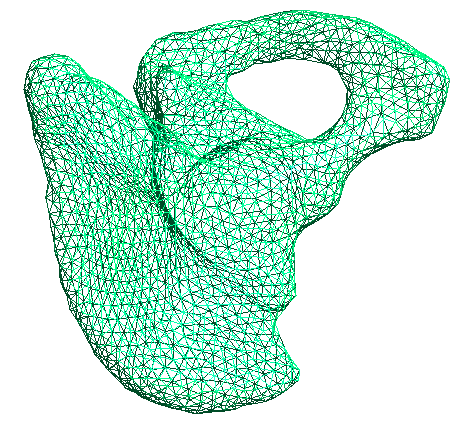
\includegraphics[width=4.5cm]{pngs/mymesh/pelvis_stl.png}
\caption{Pelvis before remesh (stl)}
\end{minipage}
\begin{minipage}[b]{.50\linewidth}
\centering
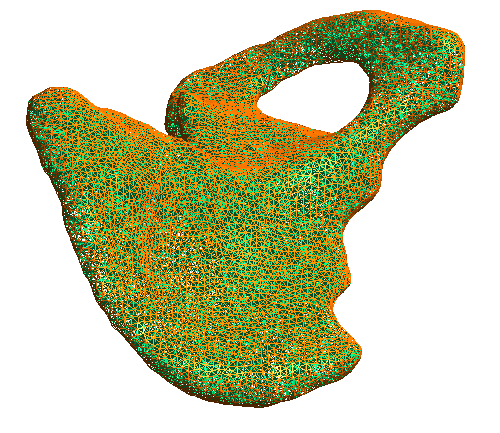
\includegraphics[width=4.5cm]{pngs/mymesh/pelvis_msh.png}
\caption{Pelvis after remesh (msh)}
\end{minipage}
\end{figure}

\end{itemize}


\section{Language for Partial Differential Equations}
\label{faq:PDE}

\subsection{What is the difference between using the "vf::project" function and solve a weak projection problem ?}

To make it clear, let's considerate that we want to project a $\mathbb{P}_1$ scalar function $\sigma$ on a $\mathbb{P}_0$ space. We have two alternatives to do it :
\begin{itemize}
\item Computing the $\mathcal{L}_2$ projection of $\sigma$ onto the space \newline
Here $kappa$ and $v$ are $\mathbb{P}_0$ functions :
\begin{lstlisting}
Matrix_M=integrate(elements(mesh), idt(kappa) * id(v));
Vector_F=integrate(elements(mesh), idv(sigma) * id(v));
\end{lstlisting}

\item Use the project function \lstinline!vf::project! \newline
This function does a nodal projection : at the dof point the projection will be \underline{exactly} equal to the projected function $\sigma$. It works as follow
\begin{lstlisting}
kappa=vf::project(P0_space, elements(mesh), idv(sigma));
\end{lstlisting}
\end{itemize}

These two projections are in general different, if you compare the values in the vector, they will be (slightly) different. However as $h \rightarrow 0$ they should both converge to the $\sigma$ function.


\subsection{How to do a quick L2 projection of an expression ?}
Let say that we have created two spaces, one scalar and one vectorial, we call them $\displaystyle{X_h}$ and $\displaystyle{X_{hVec}}$ and one wants to project some expressions on those spaces. \newline \newline
For example, we want to project $\displaystyle{(x,y) \rightarrow \sqrt{x^2 - y^2} -1}$ on the scalar space and $\displaystyle{(-2y, \cos{x})}$ on the vectorial space.
First of all, one has to create projectors for the scalar and vectorial spaces, the code reads as follow :
\begin{lstlisting}
#include <feel/feeldiscr/projector.hpp>
auto l2p = projector(Xh, Xh);
auto l2pVec = projector(XhVec, XhVec);
\end{lstlisting}
You can note that \lstinline!projector(Space, Space)! returns a \lstinline!boost::shared_ptr! on a \lstinline!Projector! object which makes projecting functions on \lstinline!Space! possible.
\newline \newline
Then, one uses the function \lstinline!Projector::project(Expression)! :
\begin{lstlisting}
auto Circle = l2p->project( sqrt( pow((vf::Px()),2.0)+ pow((vf::Py()),2.0)) - 1 );

auto F = l2pVec->project( -2 * Py() * oneX() + cos(vf::Px()) * oneY() );
\end{lstlisting}
Here you can note that the types of \lstinline!Circle! and \lstinline!F! are respectively : $X_{h}\_type::element\_type$ and $X_{hVec}\_type::element\_type$
\newline
An equivalent way to write it is to use the \lstinline!Projector::operator()(Expression)! :
\begin{lstlisting}
auto Circle = (*l2p)( sqrt( pow((vf::Px()),2.0)+ pow((vf::Py()),2.0)) - 1 );

auto F = (*l2pVec)( -2 * Py() * oneX() + cos(vf::Px()) * oneY() );
\end{lstlisting}
\lstinline!Projector::operator()! accepts many types of arguments, see \lstinline!feel/feeldiscr/projector.hpp! for details.



\subsection{How to compose \feel operators ?}

Let's considerate that we have created two spaces, one scalar $X_h$ and one vectorial $X_{hVec}$. We also have two vectors $a$ and $b$ (of type $X_{h}\_type::element\_type$).

One wants to do the following operation : $div( grad(a*b))$. The following expression is \textbf{not} yet implemented in \feel :
\begin{lstlisting}
divv( gradv( idv(a) * idv(b) ) )
\end{lstlisting}
One has to do intermediate projections to compose the operators. Using the Projector class, the code reads :
\begin{lstlisting}
#include <feel/feeldiscr/projector.hpp>

// create projectors on Xh and XhVec spaces
auto l2p = projector(Xh, Xh);
auto l2pVec = projector(XhVec, XhVec);

auto ab = l2p->project( idv(a)*idv(b) );
auto grad_ab = l2pVec->project( gradv(ab) );
auto div_grad_ab = l2p->project( divv(grad_ab) );
\end{lstlisting}
Here \lstinline!div_grad_ab! has the type $X_{h}\_type::element_type$. There is an equivalent but verboseless way to write this composition : use the \lstinline!Projector::operator()! which accepts has argument an expression or an \lstinline!element_type!. So one could write :
\begin{lstlisting}
#include <feel/feeldiscr/projector.hpp>

//create projectors on Xh and XhVec spaces
auto l2p = projector(Xh, Xh);
auto l2pVec = projector(XhVec, XhVec);

auto div_grad_ab = (*l2p)( divv( (*l2pVec)( gradv( (*l2p)(idv(a)*idv(b)) ) ) ) );
\end{lstlisting}
the * is needed before \lstinline!l2p! or \lstinline!l2pVec! since there are \lstinline!boost::shared_ptr! objects. One could also create directly \lstinline!Projector! objects :
\begin{lstlisting}
Projector<Xh_type, Xh_type> l2p(Xh, Xh);

auto ab = l2p(idv(a)*idv(b));
\end{lstlisting}


%%% Local Variables:
%%% coding: utf-8
%%% mode: latex
%%% TeX-PDF-mode: t
%%% TeX-parse-self: t
%%% x-symbol-8bits: nil
%%% TeX-auto-regexp-list: TeX-auto-full-regexp-list
%%% TeX-master: "feelpp-manual"
%%% ispell-local-dictionary: "american"
%%% End:


\chapter{Random notes}
\label{cha:random-notes}

\section{Linear Algebra with PETSC}

\subsection{Using the Petsc Backend: recommended}

Using the Petsc backend is recommended. To do that type in the command line
\begin{lstlisting}
    myprog --backend=petsc
  \end{lstlisting}
  then you can change the type of solvers and preconditioners by
  adding Petsc options at \emph{the end of the command lines}, for example
\begin{verbatim}
-pc_type lu
\end{verbatim}
  will actually solve the problem in one iteration of an iterative solver
  (p.ex. gmres).
  \begin{equation}
    \label{notes:eq:1}
    P A x = P B
  \end{equation}
  where $P \approx A^{-1}$. Here $A$ is decomposed in $LU$ form and
  (\ref{notes:eq:1}) is solved in one iteration.

\subsection{List of solvers and preconditioners}
\label{sec:list-solv-prec}

List of some iterative solvers (Krylov subspace)
\begin{itemize}
\item cg, bicg
\item gmres, fgmres, lgmres
\item bcgs, bcgsl
\item see petsc/petscksp.h for more
\end{itemize}

List of some preconditioners
\begin{itemize}
\item lu, choleski
\item jacobi, sor
\item ilu, icc
\item see petsc/petscpc.h for more
\end{itemize}

\subsection{What is going on in the solvers?}
\label{sec:what-going-solvers}

In order to monitor what is going on (iterations, residual...) Petsc
provides some monitoring options
\begin{verbatim}
-ksp_monitor
\end{verbatim}
For example
\begin{verbatim}
myprog -backend=petsc -ksp_monitor -pc_type lu
\end{verbatim}
it should show only one iteration.

See {\tiny\texttt{http://www.mcs.anl.gov/petsc/petsc-as/snapshots/petsc-current/docs/manualpages/KSP/KSPMonitorSet.html}} for more details

\section{Numerical Schemes}
\label{sec:numerical-schemes}

\subsection{Stokes problem formulation and the pressure}
\label{sec:stok-probl-form}

\subsection{The Stokes problem}
\label{sec:stokes-problem}

Consider the following problem,
\begin{equation}
  \label{notes:eq:16}
  \mbox{Stokes: }\left\{
    \begin{array}{rcc}
      -\mu\Delta\mathbf{u} +
      \nabla p =
      \mathbf{f}\\
      \nabla\cdot\mathbf{u} = 0\\
      \mathbf{u}|_{\partial \Omega} = 0
    \end{array}
  \right.
\end{equation}
where $\Omega \subset \mathbb{R}^d$. There are no boundary condition
on the pressure. This problem is ill-posed, indeed we only control the
pressure through its gradient $\nabla p$. Thus if $(\mathbf{u},p)$ is
a solution, then $(\mathbf{u},p+c)$ is also a solution with $c$ any
constant. This comes from the way the problem is posed: the box is
closed and it is not possible to determine the pressure inside. The
remedy is to impose arbitrarily a constraint on the pressure, e.g. its
mean value is zero. In other words, we add this new equation to the
problem (\ref{notes:eq:16})
\begin{equation}
  \label{notes:eq:17}
  \int_\Omega p = 0
\end{equation}
\begin{remark}[The Navier-Stokes case]
  This is also true for the incompressible Navier-Stokes equations. We
  chose Stokes to simplify the exposure.
\end{remark}

\subsection{Reformulation}
  In order to impose the condition~(\ref{notes:eq:17}), we introduce a new
  unknown, a Lagrange multiplier, $\lambda \in \mathbb{R}$ and modify
  the incompressibility equation. Our problem reads now, find
  $(\mathbf{u},p,\lambda)$ such
  that
    \begin{equation}
      \label{notes:eq:18}
    \mbox{Stokes 2: }\left\{
      \begin{array}{rcl}
        -\mu\Delta\mathbf{u} +
        \nabla p &=&
        \mathbf{f}\\
        \nabla\cdot\mathbf{u} + \lambda &=& 0\\
        \mathbf{u}|_{\partial \Omega} &=& 0\\
        \int_\Omega p &=& 0
      \end{array}
    \right.
\end{equation}
\begin{remark}[The pressure as Lagrange multiplier]
  The pressure field $p$ can actually be seen as a Lagrange multiplier
  for the velocity $\mathbf{u}$ in order to enforce the constraint
  $\nabla \cdot \mathbf{u} = 0$. $\lambda$ will play the same role but
  for the pressure to enforce the condition (\ref{notes:eq:17}). As $h
  \rightarrow 0$, $\lambda \rightarrow 0$ as well as the divergence of
  $\mathbf{u}$. Note also that $\int_\Omega \nabla \cdot \mathbf{u}
  \approx - \int_\Omega \lambda$ from the second equation.
\end{remark}

\subsection{Variational formulation}
\label{sec:vari-form}

The variational formulation now reads: find $(\mathbf{u}, p,
\lambda) \in \mathbf{H}^1_0(\Omega) \times L^2_0(\Omega) \times
\mathbb{R}$ such that for all $(\mathbf{v}, q, \eta) \in
\mathbf{H}^1_0(\Omega) \times L^2_0(\Omega) \times \mathbb{R}$

\begin{equation}
  \label{notes:eq:20}
  \mbox{Stokes 3: }\left\{
    \begin{array}{rcl}
      \int_\Omega \Big(\nabla \mathbf{u} \colon \nabla \mathbf{v} + \nabla \cdot \mathbf{v} p\Big) &=& \int_\Omega \mathbf{f} \cdot \mathbf{v}\\
      \int_\Omega \Big(\nabla\cdot\mathbf{u} q + \lambda q\Big)   &=& 0\\
      \int_\Omega p \eta &=& 0
    \end{array}
  \right.
\end{equation}

Summing up all three equations we get the following condensed formulation:

\begin{equation}
  \label{notes:eq:19}
  \int_\Omega \nabla \mathbf{u} \colon \nabla \mathbf{v} + \nabla \cdot \mathbf{v} p + \nabla \cdot \mathbf{u} q + \lambda q + \eta p = \int_\Omega \mathbf{f} \cdot \mathbf{v}
\end{equation}
where $\mathbf{H}^1_0(\Omega)= \Big\{ \mathbf{v} \in \mathbf{L}^2(\Omega), \nabla \mathbf{v} \in [L^2(\Omega)]^{d\times d},\ \mathbf{v} = 0\ \text{on}\ \partial \Omega \Big\}$,
$L^2_0(\Omega)= \Big\{ v \in L^2(\Omega),\ \int_\Omega v = 0\Big\}$, and
$\mathbf{L}^2(\Omega)= \Big\{ \mathbf{v} \in [L^2(\Omega)]^d\Big\}$ that is to say each component of a  vector field of $\mathbf{L}^2(\Omega)$ are in $L^2(\Omega)$.


\subsection{Implementation}
\label{sec:implementation}

  \begin{lstlisting}
/*basis*/
typedef Lagrange<Order, Vectorial> basis_u_type; // velocity
typedef Lagrange<Order-1, Scalar> basis_p_type; // pressure
typedef Lagrange<0, Scalar> basis_l_type; // multipliers
typedef bases<basis_u_type, basis_p_type, basis_l_type> basis_type;
/*space: product of the velocity, pressure and multiplier spaces*/
typedef FunctionSpace<mesh_type, basis_type, value_type> space_type;
// ...
space_ptrtype Xh = space_type::New( mesh );
element_type U( Xh, "u" );
element_type V( Xh, "v" );
element_0_type u = U.element<0>();
element_0_type v = V.element<0>();
element_1_type p = U.element<1>();
element_1_type q = V.element<1>();
element_2_type lambda = U.element<2>();
element_2_type nu = V.element<2>();
// ...
sparse_matrix_ptrtype D( M_backend->newMatrix( Xh, Xh ) );
form2( Xh, Xh, D, _init=true )=
   integrate( elements(mesh), im,
             // $\nabla \mathbf{u} \colon \nabla \mathbf{v}$
              mu*trace(deft*trans(def))
              // $\nabla \cdot \mathbf{v} p + \nabla \cdot \mathbf{u} q$
              - div(v)*idt(p) + divt(u)*id(q)
              // $\lambda q + \eta p$
              +id(q)*idt(lambda) + idt(p)*id(nu) );
// ...
  \end{lstlisting}


\subsection{Fix point iteration for Navier-Stokes}
\label{sec:fix-point-iteration}

\subsubsection{Steady incompressible Navier-Stokes equations}
  Consider the following steady incompressible Navier-Stokes
  equations, find $(\mathbf{u},p)$ such that
  \begin{equation}
    \label{notes:eq:7}
    \begin{split}
      \underbrace{\rho \mathbf{u} \cdot \nabla \mathbf{u}}_{\text{convection}} - \underbrace{\nu \Delta  \mathbf{u}}_{\text{diffusion}} + \nabla p &=  \mathbf{f} \ \text{on}\ \Omega \\
      \nabla \cdot \mathbf{u} &= 0 \\
      \mathbf{u} &= \mathbf{0}\ \text{on}\ \partial \Omega
    \end{split}
  \end{equation}
  where $\rho$ is the density of the fluid, $\nu$ is the dynamic
  viscosity of the fluid(la viscosité cinématique $\eta = \nu/\rho$) and $\mathbf{f}$ is the external force
  density applied to the fluid, (e.g. $\mathbf{f}=-\rho g \mathbf{e}_2$ with $\mathbf{e}_2=(0,1)^T$ ).  This equation system is nonlinear due
  to the $\mathbf{u} \cdot \nabla \mathbf{u}$ convection term. A
  simple approach to solve~(\ref{notes:eq:7}) is to use a fix point
  algorithm.


The fixpoint algorithm for NS reads as follows, find
$(\mathbf{u}^{(k)},p^{(k)})$ such that
    \begin{equation}
      \label{notes:eq:13}
    \begin{split}
      \rho\mathbf{u}^{(k-1)} \cdot \nabla \mathbf{u}^{(k)} - \nu \Delta  \mathbf{u}^{(k)} + \nabla p^{(k)} &= \mathbf{f} \ \text{on}\ \Omega \\
      \nabla \cdot \mathbf{u}^{(k)} &= 0 \\
      \mathbf{u}^{(k)} &= 0\ \text{on}\ \partial \Omega\\
      (\mathbf{u}^{(0)},p^{(0)}) &= (\mathbf{0},0)
    \end{split}
  \end{equation}
  The system~(\ref{notes:eq:13}) is now linear at each iteration $k$ and we
  can write the variational formulation accordingly. A stopping
  criterium is for example that
  $\|\mathbf{u}^{k}-\mathbf{u}^{(k-1)}\|+\|p^{k}-p^{(k-1)}\| <
  \epsilon$ where $\epsilon$ is a given tolerance (e.g. $1e-4$) and
  $\|\cdot\|$ is the $L_2$ norm.

  Here is the implementation using Life:

  \begin{lstlisting}
    // define some tolerance $\epsilon$
    epsilon = 1e-4;
    // set $(\mathbf{u}^{(0)},p^{(0)})$ to $(\mathbf{0},0)$
    velocity_element_type uk(Xh);
    velocity_element_type uk1(Xh);
    pressure_element_type pk(Ph);
    pressure_element_type pk1(Ph);
    // by default uk1, uk and pk,pk1 are initialized to 0

    // assemble the linear form associated to $\mathbf{f}$
    // store in vector $F$, it does not change over the iterations

    // iterations to find $(\mathbf{u}^{(k)},p^{(k)})$
    do
    {
      // save results of previous iterations
      uk1 = uk;
      pk1 = pk;

      //assemble for bilinear form  associated to
      // $\rho\mathbf{u}^{(k-1)} \cdot \nabla \mathbf{u}^{(k)} - \nu \Delta  \mathbf{u}^{(k)} + \nabla p^{(k)}$
      // store in matrix $A^{(k)}$

      // solve the system $A^{(k)} X = F$ where $X = (\mathbf{u}^{(k)},p^{(k)})^T$

      // use uk,uk1 and pk,pk1 to compute the error estimation at each iteration
      error = $\|\mathbf{u}^{k}-\mathbf{u}^{(k-1)}\|+\|p^{k}-p^{(k-1)}\|$
    } while( error > epsilon );

  \end{lstlisting}

\subsection{A Fix point coupling algorithm}
\label{sec:coupling-algorithm}

\subsubsection{Coupling fluid flow and heat transfer: problem}
  Recall that we have to solve two coupled problems :

  $$
  \mbox{Heat(\textbf{u}) }\left\{
  \begin{array}{rcc}
    - \kappa\Delta T + \mathbf{u}\cdot\nabla T &=& 0 \\
    T|_{\Gamma_1} &=& T_0 \\
    \frac{\partial T}{\partial \mathbf{n}}|_{\Gamma_3} &=&1 \\
    \frac{\partial T}{\partial \mathbf{n}}|_{\Gamma_2,\Gamma_4} &=& 0
  \end{array}
  \right.
  $$

  and

  $$\mbox{Stokes(T) : }\left\{
    \begin{array}{rcc}
      -\nu\Delta\mathbf{u} +
      \frac{1}{\rho}\nabla p =
      \mathbf{F}\\
      \nabla\cdot\mathbf{u} = 0\\
      \mathbf{u}|_{\partial \Omega} = 0
    \end{array}
  \right.
  $$

Where $\mathbf{F}$ can be taken as $
 \left(
  \begin{array}{c}
    0 \\
    \beta(T-T_0)
  \end{array}
\right)
$
for some $\beta > 0$. $\beta$ is called the \emph{dilatation coefficient}.

\subsubsection{Coupling fluid flow and heat transfer: algorithm}
Here is a simple algorithm fix point strategy in pseudo-code:
\begin{lstlisting}
   double tol = 1.e-6;
   int maxIter = 50;
   //Initial guess Un = 0
   do
   {
     // Find Tn solution of Heat(Un)
     // Find Unp1 solution of Stokes(Tn)
     // compute stopTest = norme(Unp1 - Un)
     // Un = Unp1
   }while((stopTest < tol) && (niter <= maxIter));
\end{lstlisting}

\begin{remark}[The unsteady case]
  To solve the unsteady problems, one can insert the previous loop in
  the one dedicated to time discretization
\end{remark}

\subsection{A Newton coupling algorithm}
\label{sec:newt-coupl-algor}

\subsubsection{A fully coupled scheme}

  Another possiblity is to use a Newton method which allows us to
  solve the full nonlinear problem coupling velocity, pressure and
  temperature
  \begin{equation}
    \label{notes:eq:21}
    \text{Find}\ X\ \text{such that}\ F(X) = 0
  \end{equation}
  the method is iterative and reads, find $X^{(n+1)}$ such that
  \begin{equation}
    \label{notes:eq:22}
    J_F(X^{(n)})( X^{(n+1)}-X^{(n)}) = - F (X^{(n)})
  \end{equation}
  starting with $X^{(0)} = \mathbf{0}$ or some other initial value and
  where $J_F$ is the jacobian matrix of $F$ evaluated at
  $X=((u_i)_i,(p_i)_i,(\theta_i)_i)^T$.  For any $\phi_k, \psi_l$ and
  $\rho_m$ the \emph{test} functions associated respectively to velocity,
  pressure and temperature, our full system reads, Find $X=((u_i)_i,(p_i)_i,(\theta_i)_i)^T$ such that
  \begin{equation}
    \label{notes:eq:23}
    \begin{array}{rll}
      F_1((u_i)_i,(p_i)_i,(\theta_i)_i)&=\sum_{i,j} u_i u_j a(\phi_i,\phi_k,\phi_j) - \sum_i p_i b(\phi_k,\psi_i) + \sum_i \theta_i c(\rho_i, \phi_k)+\sum_i u_i d(\phi_i,\phi_k)  &= 0\\
      F_2((u_i)_i,(p_i)_i,(\theta_i)_i)&=\sum_i u_i b(\phi_i,\psi_l) &=0\\
      F_3((u_i)_i,(p_i)_i,(\theta_i)_i)&=\sum_{i,j} u_i\theta_j e(\phi_i,\rho_j,\rho_m) + \sum_i \theta_i f(\rho_i,\rho_m)-g(\rho_m) &=  0
    \end{array}
  \end{equation}
  where $F=(F_1,F_2,F_3)^T$ and
  \begin{equation}
    \label{notes:eq:26}
    \begin{array}{rl}
    a(\mathbf{u},\mathbf{v},\beta) &= \int_\Omega \mathbf{v}^T ((\nabla \mathbf{u} )\beta)\\
    b(\mathbf{v},p) &= \int_\Omega p (\nabla \cdot \mathbf{v}) - \int_{\partial \Omega} \mathbf{v}\cdot\mathbf{n} p\\
      c(\theta,\mathbf{v})&= \int_\Omega \theta \mathbf{e}_2 \cdot \mathbf{v}\\
      d(\mathbf{u},\mathbf{v}) &= \frac{1}{\sqrt{\mathrm{Gr}}} \Big(\int_\Omega \nabla \mathbf{u} \colon (\nabla \mathbf{v})^T - \int_{\partial \Omega} ((\nabla \mathbf{u}) \mathbf{n})\cdot \mathbf{v}\Big)\\
      e(\mathbf{u},\theta,\chi) &= \int_\Omega (\mathbf{u}\cdot \nabla \theta) \chi \\
      f(\theta,\chi) &=\frac{1}{\sqrt{\mathrm{Gr}}\mathrm{Pr}} \Big( \int_\Omega \nabla \theta \cdot \nabla \chi - \int_{\Gamma_1} (\nabla \theta \cdot \mathbf{n} ) \chi \Big)\\
      g(\chi) &=\frac{1}{\sqrt{\mathrm{Gr}}\mathrm{Pr}} \int_{\Gamma_3} \chi
    \end{array}
  \end{equation}
  \begin{remark}
    Note that the boundary integrals are kept in order to apply the
    weak Dirichlet boundary condition trick, see next section~\ref{sec:weak-dirichl-boud}.
  \end{remark}

\subsubsection{Jacobian matrix}
  In order to apply the newton scheme, we need to compute the jacobian
  matrix $J_F$ by deriving each equation with respect to each
  unknowns, ie $u_i, p_i$ and $\theta_i$.
  Consider the first equation
  \begin{itemize}
  \item Deriving the first equation with respect to $u_i$ we get
    \begin{equation}
      \label{notes:eq:30}
      \frac{\partial F_1}{\partial u_i} = \sum_j u_j a(\phi_i,\phi_k,\phi_j) + \sum_i u_i a(\phi_i,\phi_k,\phi_j) + d(\phi_i,\phi_k)
    \end{equation}
  \item Deriving the first equation with respect to $p_i$ we get
    \begin{equation}
      \label{notes:eq:30}
      \frac{\partial F_1}{\partial p_i} =  -b(\phi_k,\psi_l)
    \end{equation}
  \item Deriving the first equation with respect to $\theta_i$ we get
    \begin{equation}
      \label{notes:eq:30}
      \frac{\partial F_1}{\partial \theta_i} = c(\rho_i,\rho_k)
    \end{equation}

  \end{itemize}
  Consider the second equation, only the derivative with respect to $u_i$ is non zero.
  \begin{equation}
    \label{notes:eq:31}
    \frac{\partial F_2}{\partial u_i} = b(\phi_i,\psi_l)
  \end{equation}
  Finally the third component
  \begin{itemize}
  \item Deriving with respect to $u_i$
    \begin{equation}
      \label{notes:eq:33}
      \frac{\partial F_3}{\partial u_i} = \sum_j \theta_j e(\phi_i,\rho_j,\rho_m)
    \end{equation}
  \item Deriving with respect to $p_i$,
    \begin{equation}
      \label{notes:eq:34}
      \frac{\partial F_3}{\partial p_i} = 0
    \end{equation}
  \item Deriving with respect to $theta_i$,
    \begin{equation}
      \label{notes:eq:35}
      \frac{\partial F_3}{\partial \theta_i} = \sum_j u_j e(\phi_j,\rho_i,\rho_m) + f(\rho_i,\rho_m)
    \end{equation}
  \end{itemize}
  \begin{equation}
    \label{notes:eq:35}
    J_F =
    \begin{pmatrix}
      \frac{\partial F_1}{\partial u_i} & \frac{\partial F_1}{\partial p_i} & \frac{\partial F_1}{\partial \theta_i} \\
      {\frac{\partial F_2}{\partial u_i}} & {\frac{\partial F_2}{\partial p_i}}(=0) & {\frac{\partial F_2}{\partial \theta_i}}(=0) \\
      \frac{\partial F_3}{\partial u_i} & {\frac{\partial F_3}{\partial p_i}}(=0) & \frac{\partial F_3}{\partial \theta_i}
    \end{pmatrix}
  \end{equation}
  In order to implement $J_F$ and solve (\ref{notes:eq:22}), $J_F$ can be
  expressed as the matrix associated with the discretisation of
  \begin{equation}
    \label{notes:eq:37}
    \begin{array}{rl}
      a(\mathbf{u},\mathbf{v},\beta_1) + a(\beta_1, \mathbf{v}, \mathbf{u})+d(\mathbf{u},\mathbf{v})-b(\mathbf{v},p)+c(\theta,\mathbf{v}) &= 0\\
      b(\mathbf{u},q)&=0\\
      e(\beta_1,\theta,\chi)+f(\theta,\chi)+e(\mathbf{u},\beta_2,\chi)&=0\\
    \end{array}
  \end{equation}
  where $\beta_1 = u^{(n)}$, $\beta_2=\theta^{(n)}$ are known from the
  previous Newton iteration, indeed $J_F$ is actually evaluated in $X^{(n)}$.

\subsubsection{Life Implementation}
  Now we use the Life non linear framework in order to implement our
  Newton scheme~(\ref{notes:eq:22}).
  We need to define two new functions in our application
  \begin{itemize}
  \item \texttt{updateJacobian(X,J)} which takes as input \texttt{X}$=X^{(n)}$ and returns the matrix \texttt{J=}$J_F(X^{(n)})$
  \item \texttt{updateResidual(X,R)} which takes as input \texttt{X}$=X^{(n)}$ and returns the vector \texttt{R=}$F(X^{(n)})$
  \end{itemize}

  \begin{remark}{Backend}
    Only the PETSC backend supports the nonlinear solver framework.
    Use  in the command line like in the first section
    \begin{lstlisting}
      --backend=petsc
    \end{lstlisting}
  \end{remark}

  Here is a snippet of code that implements the nonlinear framework.
  \begin{lstlisting}
    class MyApp
    {
      public:
      void run();
      void updateResidual( const vector_ptrtype& X, vector_ptrtype& R );
      void updateJacobian( const vector_ptrtype& X, sparse_matrix_ptrtype& J);
      void solve( sparse_matrix_ptrtype& D, element_type& u, vector_ptrtype& F );
      private:

      backend_ptrtype M_backend;
      sparse_matrix_ptrtype M_jac;
      vector_ptrtype M_residual;
    };

    void
    MyApp::run()
    {
      // ...

      // plug the updateResidual and updateJacobian functions
      // in the nonlinear framework
      M_backend->nlSolver()->residual = boost::bind( &self_type::updateResidual,
                                                     boost::ref( *this ), _1, _2 );
      M_backend->nlSolver()->jacobian = boost::bind( &self_type::updateJacobian,
                                                     boost::ref( *this ), _1, _2 );

      vector_ptrtype U( M_backend->newVector( u.functionSpace() ) );
      *U = u;
      vector_ptrtype R( M_backend->newVector( u.functionSpace() ) );
      this->updateResidual( U, R );
      sparse_matrix_ptrtype J;
      this->updateJacobian( U, J );
      solve( J, u, R );

      *U = u;
      this->updateResidual( U, R );
      // R(u) should be small
      std::cout << "R( u ) = " << M_backend->dot( U, R ) << "\n";


    }
    void
    MyApp::solve( sparse_matrix_ptrtype& D, element_type& u, vector_ptrtype& F )
    {
      vector_ptrtype U( M_backend->newVector( u.functionSpace() ) );
      *U = u;
      M_backend->nlSolve( D, U, F, 1e-10, 10 );
      u = *U;
    }
    void
    MyApp::updateResidual( const vector_ptrtype& X, vector_ptrtype& R )
    {
      // compute R(X)

      R=M_residual;
    }
    void
    MyApp::updateJacobian( const vector_ptrtype& X, vector_ptrtype& R )
    {
      // compute J(X)

      J=M_jac;
    }
  \end{lstlisting}
  see \texttt{bratu.cpp} or \texttt{nonlinearpow.cpp} for example.


\section{Weak Dirichlet boudary conditions}
\label{sec:weak-dirichl-boud}

\subsection{Basic idea}

\subsubsection{Weak treatment}
  In order to treat the boundary conditions uniformly (i.e. the same
  way as Neumann and Robin Conditions), we wish to treat the Dirichlet
  BC (e.g. $u=g$) weakly.

  \begin{remark}{Initial Idea}
    add the penalisation term $\int_{\partial \Om{}} \mu( u - g
    )$ where $\mu$ is a constant. But this is not enough, this is not consistent with the
    initial formulation.
  \end{remark}

  One can use the Nitsche ``trick'' to implement weak Dirichlet conditions.
  \begin{itemize}
  \item write the equations in conservative form (i.e. identify the flux);
  \item add the terms to ensure consistency (i.e the flux on the boundary);
  \item symmetrize to ensure adjoint consistency;
  \item add a penalisation term with factor $\gamma (u-g)/h$ that ensures
    that the solution will be set to the proper value at the boundary;
  \end{itemize}


\subsubsection{Penalisation parameter}
    \begin{remark}{Choosing $\gamma$}
    $\gamma$ must be chosen such that the coercivity(or inf-sup)
    property is satisfied. Difficult to do in general. Increase
    $\gamma$ until the BC are properly satisfied, e.g. start with
    $\gamma=1$, typical values are between 1 and 10.

    The choice of $\gamma$ is a problem specially when $h$ is small.
  \end{remark}



\subsubsection{Advantages, disadvantages}
      \begin{remark}{Weak treatment: Advantages}
        \begin{itemize}
        \item uniform(weak) treatment of all boundary conditions type
        \item if boundary condition is independant of time, the terms
          are assembled once for all
        \item the boundary condition is not enforced exactely but the
          convergence order remain optimal
        \end{itemize}
      \end{remark}
      \begin{remark}{Weak treatment: Disadvantages}
        \begin{itemize}
        \item Introduction of the penalisation parameter $\gamma$ that
          needs to be tweaked
        \end{itemize}
      \end{remark}

\subsubsection{Advantages, disadvantages}
  \begin{remark}{Strong treatment: Advantages}
    \begin{itemize}
    \item Enforce exactely the boundary conditions
    \end{itemize}
  \end{remark}
  \begin{remark}{Strong treatment : Disadvantages}
    \begin{itemize}
    \item Need to modify the matrix once assembled to reflect that
      the Dirichlet degree of freedom are actually known. Then
          even if the boundary condition is independant of time, at
          every time step if there are terms depending on time that
          need reassembly (e.g. convection) the strong treatment needs to be reapplied.
        \item it can be expensive to apply depending on the type of
          sparse matrix used, for example using CSR format setting
          rows to 0 except on the diagonal to 1 is not expensive but
          one must do that also for the columns associated with each
          Dirichlet degree of freedom and that is expensive.
        \end{itemize}
      \end{remark}

\subsection{Laplacian}
\subsubsection{Example: Laplacian}
  \begin{equation}
    \label{notes:eq:44}
    -\Delta u = f (\text{non conservative}),\ -\nabla\cdot( \nabla u )= f (\text{conservative}),\ u=g|_{\partial \Omega}
  \end{equation}
  the flux is vector $\nabla u$

  \begin{equation}
    \label{notes:eq:51}
    \int_\Omega \nabla u \cdot \nabla v + \int_{\partial \Om{}} \underbrace{-\frac{\partial u}{\partial n}v}_{\text{integration by part}} \underbrace{-\frac{\partial v}{\partial n} u}_{\text{adjoint consistency: symetrisation}}  + \underbrace{\frac{\gamma}{h} u v}_{\text{penalisation: enforce Dirichlet condition}}
  \end{equation}
  \begin{equation}
    \label{notes:eq:52}
    \int_\Omega f \nabla v + \int_{\partial \Om{}} (\underbrace{-\frac{\partial v}{\partial n} g}_{\text{adjoint consistency}} + \underbrace{\frac{\gamma}{h} v) g}_{\text{penalisation: enforce Dirichlet condition}}
  \end{equation}


\subsubsection[containsverbatim]{Example: Laplacian}
  \begin{lstlisting}
// bilinear form (left hand side)
form2( Xh, Xh, D ) +=
integrate( boundaryfaces(mesh), im_type(),
           -(gradt(u)*N())*id(v) // integration by part
           -(grad(v)*N())*idt(u) // adjoint consistency
           +gamma*id(v)*idt(u)/hFace()); // penalisation
// linear form (right hand side)
form1( Xh, F ) +=
integrate( boundaryfaces(mesh), im_type(),
           -(grad(v)*N())*g // adjoint consistency
           +gamma*id(v)*g/hFace()); // penalisation
  \end{lstlisting}


\subsection{Convection-Diffusion}
\subsubsection{Example: Convection-Diffusion}
  \begin{remark}{Convection Diffusion}
    Consider now the following problem, find $u$ such that
    \begin{equation}
      \label{notes:eq:45}
      -\Delta u + \mathbf{c} \cdot \nabla u  = f,\quad u = g|_{\partial \Om{}},\quad \nabla \cdot \mathbf{c} = 0
    \end{equation}
    under conservative form the equation reads
    \begin{equation}
      \label{notes:eq:2}
      \nabla \cdot ( -\nabla u + \mathbf{c} u ) = f,\quad u = g|_{\partial \Om{}},\quad \nabla \cdot \mathbf{c} = 0
    \end{equation}
    the flux vector field is $\mathbf{F}=-\nabla u + \mathbf{c} u$. Note that
    here the condition, $\nabla \cdot \mathbf{c} = 0$ was crucial to
    expand $\nabla \cdot (\mathbf{c} u )$ into $\mathbf{c} \cdot \nabla u$ since
    \begin{equation}
      \label{notes:eq:3}
      \nabla \cdot (\mathbf{c} u ) = \mathbf{c} \cdot \nabla u + \underbrace{u \nabla \cdot \mathbf{c}}_{=0}
    \end{equation}
  \end{remark}


\subsubsection{Weak formulation for convection diffusion}
  Multiplying by any test function $v$ and integration by
  part of (\ref{notes:eq:2}) gives
  \begin{equation}
    \label{notes:eq:4}
    \int_\Omega \nabla u \cdot \nabla v + (\mathbf{c} \cdot \nabla u)v + \int_{\partial \Omega} (\mathbf{F}\cdot \mathbf{n}) v = \int_\Omega f v
  \end{equation}
  where $\mathbf{n}$ is the outward unit normal to $\partial
  \Omega$. We now introduce the penalisation term that will ensure
  that $u \rightarrow g$ as $h \rightarrow 0$ on $\partial \Omega$. (\ref{notes:eq:4}) reads now
  \begin{equation}
    \label{notes:eq:5}
    \int_\Omega \nabla u \cdot \nabla v + (\mathbf{c} \cdot \nabla u)v + \int_{\partial \Omega} (\mathbf{F}\cdot \mathbf{n}) v + \mathbf{\frac{\gamma}{h} u v}  = \int_\Omega f v + \mathbf{\int_{\partial \Omega} \frac{\gamma}{h} g v}
  \end{equation}

  Finally we incorporate the symetrisation of the bilinear form to ensure adjoint consistency and hence proper convergence order
  \begin{equation}
    \label{notes:eq:6}
    \begin{split}
      \int_\Omega \nabla u \cdot \nabla v + (\mathbf{c} \cdot \nabla u)v +
      \int_{\partial \Omega} ((-\nabla u + \mathbf{c} u)\cdot \mathbf{n}) v+ \mathbf{((-\nabla v + \mathbf{c} v)\cdot \mathbf{n}) u} + \frac{\gamma}{h} u v  = \\
      \int_\Omega f v + \int_{\partial \Omega} \mathbf{((-\nabla v + \mathbf{c} v)\cdot \mathbf{n}) g}+ \frac{\gamma}{h} g v
    \end{split}
  \end{equation}


\subsubsection[containsverbatim]{Example: Convection-Diffusion}
  \begin{lstlisting}
// bilinear form (left hand side)
form2( Xh, Xh, D ) +=
integrate( boundaryfaces(mesh), im_type(),
           // integration by part
           -(gradt(u)*N())*id(v) + (idt(u)*trans(idv(c))*N())*id(v)
           // adjoint consistency
           -(grad(v)*N())*idt(u) + (id(v)*trans(idv(c))*N())*idt(u)
           // penalisation
           +gamma*id(v)*idt(u)/hFace());
// linear form (right hand side)
form1( Xh, F ) +=
integrate( boundaryfaces(mesh), im_type(),
           // adjoint consistency
           -(grad(v)*N())*g + (id(v)*trans(idv(c))*N())*g
           // penalisation
           +gamma*id(v)*g/hFace());
  \end{lstlisting}


\subsection{Stokes}
\subsubsection{Example: Stokes}
  \begin{remark}{Stokes}
    Consider now the following problem, find $(\mathbf{u},p)$ such that
    \begin{equation}
      \label{notes:eq:45}
      -\Delta \mathbf{u} + \nabla p  = \mathbf{f},\quad \mathbf{u} = \mathbf{g}|_{\partial \Om{}},\quad \nabla \cdot \mathbf{u} = 0
    \end{equation}
    under conservative form the equation reads
    \begin{eqnarray}
      \nabla \cdot ( -\nabla \mathbf{u} + p \mathbb{I} ) &= \mathbf{f},\label{notes:eq:8}\\
      \nabla \cdot \mathbf{u} &= 0,\label{notes:eq:10}\\
      \mathbf{u} &= \mathbf{g}|_{\partial \Om{}}\label{notes:eq:11}
    \end{eqnarray}
    where $\mathbb{I}(\mathbf{x})=
    \begin{pmatrix}
      1 & 0\\
      0 & 1
    \end{pmatrix}\text{(in 2D)}
    \ \forall \mathbf{x} \in \Omega$ is the identity tensor(matrix) field $\in
    \mathbb{R}^{d\times d}$. The flux tensor field is
    $\mathbf{F}=-\nabla \mathbf{u} + p\mathbb{I}$. Indeed we have  the
    following relation, if $\mathbb{M}$ is a tensor (rank 2) field and $\mathbf{v}$ is a vector field
    \begin{equation}
      \label{notes:eq:12}
      \nabla \cdot ( \mathbb{M} \mathbf{v} ) = (\nabla \cdot \mathbb{M}) \cdot \mathbf{v} + \mathbb{M} \colon (\nabla \mathbf{v})
    \end{equation}
    where $\mathbb{M} \colon (\nabla \mathbf{v}) =
    \mathrm{trace}(\mathbb{M}*\nabla \mathbf{v}^T)$, $*$ is the
    matrix-matrix multiplication and $\nabla \cdot \mathbb{M}$ is the
    vector field with components the divergence of each row of
    $\mathbb{M}$. For example $\nabla \cdot (p\ \mathbb{I})=\nabla \cdot
    \begin{pmatrix}
      p & 0 \\
      0 & p
    \end{pmatrix}(\text{in 2D}) =  \nabla p$.
  \end{remark}


\subsubsection{Weak formulation for Stokes}
  Taking the scalar product of (\ref{notes:eq:8}) by any test function
  $\mathbf{v}$ (associated to velocity) and multiplying (\ref{notes:eq:10})
  by any test function $q$ (associated to pressure), the variational
  formulation of (\ref{notes:eq:8}) reads, thanks to~(\ref{notes:eq:12}),
  \begin{equation}
    \label{notes:eq:9}
    \int_\Omega \nabla \mathbf{u} \colon \nabla \mathbf{v} +  p \nabla \cdot \mathbf{v} + \int_{\partial \Omega} ( (-\nabla \mathbf{u} + p\mathbb{I}) \mathbf{n}) \cdot \mathbf{v} = \int_\Omega \mathbf{f} \cdot \mathbf{v}
  \end{equation}
  where $\mathbf{n}$ is the outward unit normal to $\partial
  \Omega$. We now introduce the penalisation term that will ensure
  that $\mathbf{u} \rightarrow \mathbf{g}$ as $h \rightarrow 0$ on $\partial \Omega$. (\ref{notes:eq:9}) reads now
  \begin{equation}
    \label{notes:eq:14}
    \int_\Omega \nabla \mathbf{u} \colon \nabla \mathbf{v} +  p \nabla \cdot \mathbf{v} + \int_{\partial \Omega} ((-\nabla \mathbf{u} + p\mathbb{I}) \mathbf{n})\cdot \mathbf{v} + \mathbf{\frac{\gamma}{h} \mathbf{u}\cdot \mathbf{v}}  = \int_\Omega \mathbf{f} \cdot \mathbf{v} + \mathbf{\int_{\partial \Omega} \frac{\gamma}{h} \mathbf{g} \cdot \mathbf{v}}
  \end{equation}

  Finally we incorporate the symetrisation of the bilinear form to ensure adjoint consistency and hence proper convergence order
  \begin{equation}
    \label{notes:eq:15}
    \begin{split}
      \int_\Omega \nabla \mathbf{u} \colon \nabla \mathbf{v} +  p \nabla \cdot \mathbf{v} +
      \int_{\partial \Omega} ((-\nabla \mathbf{u} + p\mathbb{I}) \mathbf{n})\cdot \mathbf{v} + ((-\nabla \mathbf{v} + q\mathbb{I}) \mathbf{n})\cdot \mathbf{u} + \frac{\gamma}{h} \mathbf{u}\cdot \mathbf{v} = \\
      \int_\Omega \mathbf{f} \cdot \mathbf{v} + \int_{\partial \Omega} ((-\nabla \mathbf{v} + q\mathbb{I}) \mathbf{n})\cdot \mathbf{g} + \frac{\gamma}{h} \mathbf{g} \cdot \mathbf{v}
    \end{split}
  \end{equation}


\subsubsection[containsverbatim]{Example: Stokes}
  \begin{lstlisting}
    // total stress tensor (trial)
    AUTO( SigmaNt, (-idt(p)*N()+mu*gradt(u)*N()) );
    // total stress tensor (test)
    AUTO( SigmaN, (-id(p)*N()+mu*grad(v)*N()) );
    // linear form (right hand side)
    form1( Xh, F ) +=
    integrate( boundaryfaces(mesh), im,
               trans(g)*(-SigmaN+gamma*id(v)/hFace() ) );
    // bilinear form (left hand side)
    form2( Xh, Xh, D )+=
    integrate( boundaryfaces(mesh), im,
               -trans(SigmaNt)*id(v)
               -trans(SigmaN)*idt(u)
               +gamma*trans(idt(u))*id(v)/hFace() );
  \end{lstlisting}



\section{Stabilisation techniques}

\subsection{Convection dominated flows}

Consider this type of problem
\begin{equation}
  \label{notes:eq:46}
  -\epsilon \Delta u + \mathbf{c} \cdot \nabla u + \gamma u = f,\quad \nabla \cdot \mathbf{c} = 0
\end{equation}
Introduce $\mathrm{Pe}=\frac{|\mathbf{c}|h}{\epsilon}$ the \emph{Péclet}
number. The dominating convection occurs when, on at least some cells,
$\mathrm{Pe} >> 1$. We talk about singularly (i.e. $\epsilon << h$)
perturbed flows.

Without doing anything wiggles occur. There are remedies  so
called \emph{Stabilisation Methods}, here some some examples:
\begin{itemize}
\item Artificial diffusion (streamline diffusion) (SDFEM)
\item Galerkin Least Squares method (GaLS)
\item Streamline Upwind Petrov Galerkin (SUPG)
\item Continuous Interior Penalty methods (CIP)
\end{itemize}

\subsection{The CIP methods}
  Add the term
  \begin{equation}
    \label{notes:eq:47}
    \sum_{F \in \Gamma_\mathrm{int} } \int_{F} \gamma\ h_F^2\ |\mathbf{c} \cdot \mathbf{n}|\  [\nabla u]  [\nabla v]
  \end{equation}
  where $\Gamma_\mathrm{int}$ is the set of internal faces where the
  $\mathrm{Pe}>>1$ (typically it is applied to all internal faces) and
  \begin{equation}
    \label{notes:eq:50}
    [\nabla u] = \nabla u \cdot \mathbf{n}|_1 + \nabla u \cdot \mathbf{n}|_2
  \end{equation}
  is the jump of $\nabla u$(scalar valued) across the face.  In the
  case of scalar valued functions
  \begin{equation}
    \label{notes:eq:53}
    [u] = u \mathbf{n}|_1 + u \mathbf{n}|_2
  \end{equation}
  \begin{remark}[Choice for $\gamma$]
    $\gamma$ can be taken in the range $[1e-2;1e-1]$. A typical value is $2.5e-2$.
  \end{remark}


\begin{lstlisting}
    // define the stabilisation coefficient expression
    AUTO( stab_coeff , ($\gamma_\beta$ abs(trans(N())*idv(beta)))*
                        vf::pow(hFace(),2.0));

    // assemble the stabilisation operator
    form2( Xh, Xh, M ) +=
     integrate(
        // internal faces of the mesh
        internalfaces(Xh->mesh()),
        // integration method
        _Q<OrderOfPolynomialToBeIntegratedExactely>,
        // stabilisation term
        stab_coeff*(trans(jumpt(gradt(u)))*jump(grad(v))));
\end{lstlisting}

\section{Interpolation}

In order to interpolate a function defined on one domain to another domain, one
can use the \lstinline{interpolate} function. The basis function of the image
space must be of \lstinline{Lagrange} type.

\begin{lstlisting}
typedef bases<Lagrange<Order, Vectorial> > basis_type; // velocity
typedef FunctionSpace<mesh_type, basis_type, value_type> space_type;
// ...
space_ptrtype Xh = space_type::New( mesh1 );
element_type u( Xh, "u" );
space_ptrtype Yh = space_type::New( mesh2 );
element_type v( Yh, "v" );

// interpolate u on mesh2 and store the result in v
interpolate( Yh, u, v );
\end{lstlisting}

%%% Local Variables:
%%% coding: utf-8
%%% mode: latex
%%% TeX-PDF-mode: t
%%% TeX-parse-self: t
%%% x-symbol-8bits: nil
%%% TeX-auto-regexp-list: TeX-auto-full-regexp-list
%%% TeX-master: "life-manual"
%%% ispell-local-dictionary: "french"
%%% End:

\chapter{GNU Free Documentation License}
\label{sec:gnu-free-docum}

		GNU Free Documentation License
		  Version 1.2, November 2002


 Copyright (C) 2000,2001,2002  Free Software Foundation, Inc.
     51 Franklin St, Fifth Floor, Boston, MA  02110-1301  USA
 Everyone is permitted to copy and distribute verbatim copies
 of this license document, but changing it is not allowed.


\section*{Preamble}

The purpose of this License is to make a manual, textbook, or other
functional and useful document "free" in the sense of freedom: to
assure everyone the effective freedom to copy and redistribute it,
with or without modifying it, either commercially or noncommercially.
Secondarily, this License preserves for the author and publisher a way
to get credit for their work, while not being considered responsible
for modifications made by others.

This License is a kind of "copyleft", which means that derivative
works of the document must themselves be free in the same sense.  It
complements the GNU General Public License, which is a copyleft
license designed for free software.

We have designed this License in order to use it for manuals for free
software, because free software needs free documentation: a free
program should come with manuals providing the same freedoms that the
software does.  But this License is not limited to software manuals;
it can be used for any textual work, regardless of subject matter or
whether it is published as a printed book.  We recommend this License
principally for works whose purpose is instruction or reference.


\section*{Applicability and definitions}
\label{sec:appl-defin}

This License applies to any manual or other work, in any medium, that
contains a notice placed by the copyright holder saying it can be
distributed under the terms of this License.  Such a notice grants a
world-wide, royalty-free license, unlimited in duration, to use that
work under the conditions stated herein.  The "Document", below,
refers to any such manual or work.  Any member of the public is a
licensee, and is addressed as "you".  You accept the license if you
copy, modify or distribute the work in a way requiring permission
under copyright law.

A "Modified Version" of the Document means any work containing the
Document or a portion of it, either copied verbatim, or with
modifications and/or translated into another language.

A "Secondary Section" is a named appendix or a front-matter section of
the Document that deals exclusively with the relationship of the
publishers or authors of the Document to the Document's overall subject
(or to related matters) and contains nothing that could fall directly
within that overall subject.  (Thus, if the Document is in part a
textbook of mathematics, a Secondary Section may not explain any
mathematics.)  The relationship could be a matter of historical
connection with the subject or with related matters, or of legal,
commercial, philosophical, ethical or political position regarding
them.

The "Invariant Sections" are certain Secondary Sections whose titles
are designated, as being those of Invariant Sections, in the notice
that says that the Document is released under this License.  If a
section does not fit the above definition of Secondary then it is not
allowed to be designated as Invariant.  The Document may contain zero
Invariant Sections.  If the Document does not identify any Invariant
Sections then there are none.

The "Cover Texts" are certain short passages of text that are listed,
as Front-Cover Texts or Back-Cover Texts, in the notice that says that
the Document is released under this License.  A Front-Cover Text may
be at most 5 words, and a Back-Cover Text may be at most 25 words.

A "Transparent" copy of the Document means a machine-readable copy,
represented in a format whose specification is available to the
general public, that is suitable for revising the document
straightforwardly with generic text editors or (for images composed of
pixels) generic paint programs or (for drawings) some widely available
drawing editor, and that is suitable for input to text formatters or
for automatic translation to a variety of formats suitable for input
to text formatters.  A copy made in an otherwise Transparent file
format whose markup, or absence of markup, has been arranged to thwart
or discourage subsequent modification by readers is not Transparent.
An image format is not Transparent if used for any substantial amount
of text.  A copy that is not "Transparent" is called "Opaque".

Examples of suitable formats for Transparent copies include plain
ASCII without markup, Texinfo input format, LaTeX input format, SGML
or XML using a publicly available DTD, and standard-conforming simple
HTML, PostScript or PDF designed for human modification.  Examples of
transparent image formats include PNG, XCF and JPG.  Opaque formats
include proprietary formats that can be read and edited only by
proprietary word processors, SGML or XML for which the DTD and/or
processing tools are not generally available, and the
machine-generated HTML, PostScript or PDF produced by some word
processors for output purposes only.

The "Title Page" means, for a printed book, the title page itself,
plus such following pages as are needed to hold, legibly, the material
this License requires to appear in the title page.  For works in
formats which do not have any title page as such, "Title Page" means
the text near the most prominent appearance of the work's title,
preceding the beginning of the body of the text.

A section "Entitled XYZ" means a named subunit of the Document whose
title either is precisely XYZ or contains XYZ in parentheses following
text that translates XYZ in another language.  (Here XYZ stands for a
specific section name mentioned below, such as "Acknowledgements",
"Dedications", "Endorsements", or "History".)  To "Preserve the Title"
of such a section when you modify the Document means that it remains a
section "Entitled XYZ" according to this definition.

The Document may include Warranty Disclaimers next to the notice which
states that this License applies to the Document.  These Warranty
Disclaimers are considered to be included by reference in this
License, but only as regards disclaiming warranties: any other
implication that these Warranty Disclaimers may have is void and has
no effect on the meaning of this License.


\section*{Verbatim copying}
\label{sec:verbatim-copying}

You may copy and distribute the Document in any medium, either
commercially or noncommercially, provided that this License, the
copyright notices, and the license notice saying this License applies
to the Document are reproduced in all copies, and that you add no other
conditions whatsoever to those of this License.  You may not use
technical measures to obstruct or control the reading or further
copying of the copies you make or distribute.  However, you may accept
compensation in exchange for copies.  If you distribute a large enough
number of copies you must also follow the conditions in section 3.

You may also lend copies, under the same conditions stated above, and
you may publicly display copies.

\section*{Copying in quantity}
\label{sec:copying-quantity}

If you publish printed copies (or copies in media that commonly have
printed covers) of the Document, numbering more than 100, and the
Document's license notice requires Cover Texts, you must enclose the
copies in covers that carry, clearly and legibly, all these Cover
Texts: Front-Cover Texts on the front cover, and Back-Cover Texts on
the back cover.  Both covers must also clearly and legibly identify
you as the publisher of these copies.  The front cover must present
the full title with all words of the title equally prominent and
visible.  You may add other material on the covers in addition.
Copying with changes limited to the covers, as long as they preserve
the title of the Document and satisfy these conditions, can be treated
as verbatim copying in other respects.

If the required texts for either cover are too voluminous to fit
legibly, you should put the first ones listed (as many as fit
reasonably) on the actual cover, and continue the rest onto adjacent
pages.

If you publish or distribute Opaque copies of the Document numbering
more than 100, you must either include a machine-readable Transparent
copy along with each Opaque copy, or state in or with each Opaque copy
a computer-network location from which the general network-using
public has access to download using public-standard network protocols
a complete Transparent copy of the Document, free of added material.
If you use the latter option, you must take reasonably prudent steps,
when you begin distribution of Opaque copies in quantity, to ensure
that this Transparent copy will remain thus accessible at the stated
location until at least one year after the last time you distribute an
Opaque copy (directly or through your agents or retailers) of that
edition to the public.

It is requested, but not required, that you contact the authors of the
Document well before redistributing any large number of copies, to give
them a chance to provide you with an updated version of the Document.

\section*{Modifications}

You may copy and distribute a Modified Version of the Document under
the conditions of sections 2 and 3 above, provided that you release
the Modified Version under precisely this License, with the Modified
Version filling the role of the Document, thus licensing distribution
and modification of the Modified Version to whoever possesses a copy
of it.  In addition, you must do these things in the Modified Version:

\begin{enumerate}
\item Use in the Title Page (and on the covers, if any) a title distinct
   from that of the Document, and from those of previous versions
   (which should, if there were any, be listed in the History section
   of the Document).  You may use the same title as a previous version
   if the original publisher of that version gives permission.
\item List on the Title Page, as authors, one or more persons or entities
   responsible for authorship of the modifications in the Modified
   Version, together with at least five of the principal authors of the
   Document (all of its principal authors, if it has fewer than five),
   unless they release you from this requirement.


\item State on the Title page the name of the publisher of the
   Modified Version, as the publisher.
\item Preserve all the copyright notices of the Document.
\item Add an appropriate copyright notice for your modifications
   adjacent to the other copyright notices.
\item Include, immediately after the copyright notices, a license notice
   giving the public permission to use the Modified Version under the
   terms of this License, in the form shown in the Addendum below.
\item Preserve in that license notice the full lists of Invariant Sections
   and required Cover Texts given in the Document's license notice.
\item Include an unaltered copy of this License.
\item Preserve the section Entitled "History", Preserve its Title, and add
   to it an item stating at least the title, year, new authors, and
   publisher of the Modified Version as given on the Title Page.  If
   there is no section Entitled "History" in the Document, create one
   stating the title, year, authors, and publisher of the Document as
   given on its Title Page, then add an item describing the Modified
   Version as stated in the previous sentence.
\item Preserve the network location, if any, given in the Document for
   public access to a Transparent copy of the Document, and likewise
   the network locations given in the Document for previous versions
   it was based on.  These may be placed in the "History" section.
   You may omit a network location for a work that was published at
   least four years before the Document itself, or if the original
   publisher of the version it refers to gives permission.
\item For any section Entitled "Acknowledgements" or "Dedications",
   Preserve the Title of the section, and preserve in the section all
   the substance and tone of each of the contributor acknowledgements
   and/or dedications given therein.
\item Preserve all the Invariant Sections of the Document,
   unaltered in their text and in their titles.  Section numbers
   or the equivalent are not considered part of the section titles.
\item Delete any section Entitled "Endorsements".  Such a section
   may not be included in the Modified Version.
\item Do not retitle any existing section to be Entitled "Endorsements"
   or to conflict in title with any Invariant Section.
\item Preserve any Warranty Disclaimers.
\end{enumerate}

If the Modified Version includes new front-matter sections or
appendices that qualify as Secondary Sections and contain no material
copied from the Document, you may at your option designate some or all
of these sections as invariant.  To do this, add their titles to the
list of Invariant Sections in the Modified Version's license notice.
These titles must be distinct from any other section titles.

You may add a section Entitled "Endorsements", provided it contains
nothing but endorsements of your Modified Version by various
parties--for example, statements of peer review or that the text has
been approved by an organization as the authoritative definition of a
standard.

You may add a passage of up to five words as a Front-Cover Text, and a
passage of up to 25 words as a Back-Cover Text, to the end of the list
of Cover Texts in the Modified Version.  Only one passage of
Front-Cover Text and one of Back-Cover Text may be added by (or
through arrangements made by) any one entity.  If the Document already
includes a cover text for the same cover, previously added by you or
by arrangement made by the same entity you are acting on behalf of,
you may not add another; but you may replace the old one, on explicit
permission from the previous publisher that added the old one.

The author(s) and publisher(s) of the Document do not by this License
give permission to use their names for publicity for or to assert or
imply endorsement of any Modified Version.


\section*{Combining documents}

You may combine the Document with other documents released under this
License, under the terms defined in section 4 above for modified
versions, provided that you include in the combination all of the
Invariant Sections of all of the original documents, unmodified, and
list them all as Invariant Sections of your combined work in its
license notice, and that you preserve all their Warranty Disclaimers.

The combined work need only contain one copy of this License, and
multiple identical Invariant Sections may be replaced with a single
copy.  If there are multiple Invariant Sections with the same name but
different contents, make the title of each such section unique by
adding at the end of it, in parentheses, the name of the original
author or publisher of that section if known, or else a unique number.
Make the same adjustment to the section titles in the list of
Invariant Sections in the license notice of the combined work.

In the combination, you must combine any sections Entitled "History"
in the various original documents, forming one section Entitled
"History"; likewise combine any sections Entitled "Acknowledgements",
and any sections Entitled "Dedications".  You must delete all sections
Entitled "Endorsements".


\section*{Collections of documents}

You may make a collection consisting of the Document and other documents
released under this License, and replace the individual copies of this
License in the various documents with a single copy that is included in
the collection, provided that you follow the rules of this License for
verbatim copying of each of the documents in all other respects.

You may extract a single document from such a collection, and distribute
it individually under this License, provided you insert a copy of this
License into the extracted document, and follow this License in all
other respects regarding verbatim copying of that document.


\section*{Aggregation with independent works}

A compilation of the Document or its derivatives with other separate
and independent documents or works, in or on a volume of a storage or
distribution medium, is called an "aggregate" if the copyright
resulting from the compilation is not used to limit the legal rights
of the compilation's users beyond what the individual works permit.
When the Document is included in an aggregate, this License does not
apply to the other works in the aggregate which are not themselves
derivative works of the Document.

If the Cover Text requirement of section 3 is applicable to these
copies of the Document, then if the Document is less than one half of
the entire aggregate, the Document's Cover Texts may be placed on
covers that bracket the Document within the aggregate, or the
electronic equivalent of covers if the Document is in electronic form.
Otherwise they must appear on printed covers that bracket the whole
aggregate.


\section*{Translation}

Translation is considered a kind of modification, so you may
distribute translations of the Document under the terms of section 4.
Replacing Invariant Sections with translations requires special
permission from their copyright holders, but you may include
translations of some or all Invariant Sections in addition to the
original versions of these Invariant Sections.  You may include a
translation of this License, and all the license notices in the
Document, and any Warranty Disclaimers, provided that you also include
the original English version of this License and the original versions
of those notices and disclaimers.  In case of a disagreement between
the translation and the original version of this License or a notice
or disclaimer, the original version will prevail.

If a section in the Document is Entitled "Acknowledgements",
"Dedications", or "History", the requirement (section 4) to Preserve
its Title (section 1) will typically require changing the actual
title.


\section*{Termination}

You may not copy, modify, sublicense, or distribute the Document except
as expressly provided for under this License.  Any other attempt to
copy, modify, sublicense or distribute the Document is void, and will
automatically terminate your rights under this License.  However,
parties who have received copies, or rights, from you under this
License will not have their licenses terminated so long as such
parties remain in full compliance.


\section*{Future revisions of this license}

The Free Software Foundation may publish new, revised versions
of the GNU Free Documentation License from time to time.  Such new
versions will be similar in spirit to the present version, but may
differ in detail to address new problems or concerns.  See
http://www.gnu.org/copyleft/.

Each version of the License is given a distinguishing version number.
If the Document specifies that a particular numbered version of this
License "or any later version" applies to it, you have the option of
following the terms and conditions either of that specified version or
of any later version that has been published (not as a draft) by the
Free Software Foundation.  If the Document does not specify a version
number of this License, you may choose any version ever published (not
as a draft) by the Free Software Foundation.


\section*{ADDENDUM: How to use this License for your documents}

To use this License in a document you have written, include a copy of
the License in the document and put the following copyright and
license notices just after the title page:

    Copyright (c)  YEAR  YOUR NAME.
    Permission is granted to copy, distribute and/or modify this document
    under the terms of the GNU Free Documentation License, Version 1.2
    or any later version published by the Free Software Foundation;
    with no Invariant Sections, no Front-Cover Texts, and no Back-Cover Texts.
    A copy of the license is included in the section entitled "GNU
    Free Documentation License".

If you have Invariant Sections, Front-Cover Texts and Back-Cover Texts,
replace the "with...Texts." line with this:

    with the Invariant Sections being LIST THEIR TITLES, with the
    Front-Cover Texts being LIST, and with the Back-Cover Texts being LIST.

If you have Invariant Sections without Cover Texts, or some other
combination of the three, merge those two alternatives to suit the
situation.

If your document contains nontrivial examples of program code, we
recommend releasing these examples in parallel under your choice of
free software license, such as the GNU General Public License,
to permit their use in free software.




%%\chapter*{List of Authors and Contributors}

\begin{itemize}
\item
  Christophe Prud'homme (Université Joseph Fourier)
\end{itemize}


\section{Master students}

\begin{itemize}
\item Baptiste Morin (UJF-Polytech)
\end{itemize}

%%% Local Variables:
%%% coding: utf-8
%%% mode: latex
%%% TeX-PDF-mode: t
%%% TeX-parse-self: t
%%% x-symbol-8bits: nil
%%% TeX-auto-regexp-list: TeX-auto-full-regexp-list
%%% TeX-master: "feel-manual"
%%% ispell-local-dictionary: "american"
%%% End:


\backmatter

\printindex

\nocite{*}
\bibliographystyle{plain}
\bibliography{../biblio/feel-manual,../biblio/feelpp,../biblio/feelpp-thesis}




\end{document}
%%% Local Variables:
%%% coding: utf-8
%%% mode: latex
%%% TeX-PDF-mode: t
%%% TeX-parse-self: t
%%% x-symbol-8bits: nil
%%% TeX-auto-regexp-list: TeX-auto-full-regexp-list
%%% TeX-master: t
%%% ispell-local-dictionary: "american"
%%% End:

